% Complete Technical Research Report. Build from the folder report/:  pdflatex Complete_Technical_Research_Report.tex  (run twice)
\documentclass[11pt,a4paper]{article}
% Shared preamble of the two documents (Director's Research Guide, Complete Technical Research Report).
\usepackage[margin=2.3cm]{geometry}
\usepackage[T1]{fontenc}
\usepackage{lmodern}
\usepackage[utf8]{inputenc}
\usepackage{microtype}
\usepackage{amsmath,amssymb}
\usepackage{graphicx}
\usepackage{booktabs,longtable,array,tabularx,multirow}
\usepackage{xcolor}
\usepackage{float}
\usepackage[labelfont=bf,font=small]{caption}
\usepackage{enumitem}
\usepackage{url}
\usepackage{fancyhdr}
\usepackage{listings}
\usepackage[most]{tcolorbox}
\usepackage{tikz}
\usetikzlibrary{positioning,arrows.meta,fit,shapes.geometric,calc,backgrounds}
\usepackage[colorlinks=true,linkcolor=blue!50!black,urlcolor=blue!50!black,citecolor=blue!50!black]{hyperref}

\definecolor{proposedblue}{HTML}{2A78D6}
\definecolor{baselineorange}{HTML}{EB6834}
\definecolor{ruleblack}{HTML}{8A8984}
\definecolor{softgreen}{HTML}{1BAF7A}
\definecolor{softred}{HTML}{E34948}
\definecolor{softviolet}{HTML}{6250D6}

\DeclareRobustCommand{\code}[1]{\texttt{\detokenize{#1}}}   % identifiers and file names (underscores allowed; robust for section titles)
\newcommand{\pth}[1]{\path{#1}}                              % file system paths (line-breakable)
\newcommand{\codename}[1]{}                                  % internal nicknames are no longer printed in running text

% Boxes used throughout
\newtcolorbox{plainwords}[1][In plain words]{enhanced,breakable,colback=blue!4,colframe=blue!45!black,fonttitle=\bfseries\small,title=#1,
  left=6pt,right=6pt,top=4pt,bottom=4pt,boxrule=0.6pt,arc=2pt}
\newtcolorbox{implicationbox}[1][Research implication]{enhanced,breakable,colback=green!5!white,colframe=green!35!black,fonttitle=\bfseries\small,title=#1,
  left=6pt,right=6pt,top=4pt,bottom=4pt,boxrule=0.6pt,arc=2pt}
\newtcolorbox{cautionbox}[1][Important to know]{enhanced,breakable,colback=red!4,colframe=red!50!black,fonttitle=\bfseries\small,title=#1,
  left=6pt,right=6pt,top=4pt,bottom=4pt,boxrule=0.6pt,arc=2pt}

% A figure with a descriptive caption followed by a plain-English reading and the research implication.
% arguments: 1 file name (without extension), 2 width as a fraction of the text width, 3 title, 4 what is shown, 5 plain-English reading, 6 research implication, 7 label
\newcommand{\explainedfigure}[7]{%
\begin{figure}[H]\centering
\includegraphics[width=#2\textwidth,height=0.56\textheight,keepaspectratio]{figures/#1.pdf}
\caption{\textbf{#3.} #4}\label{#7}
\end{figure}
\begin{tcolorbox}[enhanced,breakable,colback=gray!6,colframe=gray!55,boxrule=0.5pt,arc=2pt,left=6pt,right=6pt,top=3pt,bottom=3pt]
{\small\textbf{Plain-English reading.} #5\par\smallskip
\textbf{Research implication.} #6}
\end{tcolorbox}\medskip}

\lstset{basicstyle=\ttfamily\footnotesize,breaklines=true,frame=single,columns=fullflexible,keepspaces=true,
        showstringspaces=false,backgroundcolor=\color{black!3}}
\setlist{itemsep=2pt,topsep=3pt}
\setlength{\parindent}{0pt}
\setlength{\parskip}{5pt}
\sloppy
\emergencystretch=2em
\setcounter{tocdepth}{2}
\renewcommand{\arraystretch}{1.12}

% Flow diagram of one reinforcement-learning attempt: starting model -> initialisation -> training set-up -> training loop -> result.
% arguments: 1 starting model, 2 initialisation, 3 training set-up (environment and reward), 4 training loop (algorithm, steps), 5 result (what happened), 6 colour of the result box
\newcommand{\rlflow}[6]{%
\begin{center}
\begin{tikzpicture}[font=\scriptsize,>=Stealth,node distance=0.35cm,
  stage/.style={draw,rounded corners=2pt,fill=white,text width=2.75cm,minimum height=3.7cm,align=left,inner sep=3pt},
  result/.style={draw,rounded corners=2pt,text width=2.75cm,minimum height=3.7cm,align=left,inner sep=3pt,line width=0.8pt}]
\node[stage,fill=blue!6] (a) {\textbf{1. Starting model}\\[2pt] #1};
\node[stage,right=of a] (b) {\textbf{2. Initialisation}\\[2pt] #2};
\node[stage,right=of b] (c) {\textbf{3. Training set-up}\\[2pt] #3};
\node[stage,right=of c] (d) {\textbf{4. Training loop}\\[2pt] #4};
\node[result,right=of d,fill=#6!12,draw=#6!70!black] (e) {\textbf{5. What happened}\\[2pt] #5};
\foreach \x/\y in {a/b,b/c,c/d,d/e} \draw[->] (\x) -- (\y);
\end{tikzpicture}
\end{center}}

\newcommand{\ImOnSuccess}{0.130}
\newcommand{\ImOnLow}{0.090}
\newcommand{\ImOnHigh}{0.184}
\newcommand{\ImOnCollision}{0.200}
\newcommand{\ImOnOffroad}{0.605}
\newcommand{\ImOnTimeout}{0.065}
\newcommand{\ImOnSpeed}{9.20}
\newcommand{\ImOnEnergy}{276.6}

\pagestyle{fancy}\fancyhf{}
\fancyhead[L]{\small Complete Technical Research Report}
\fancyhead[R]{\small Driving models that read a bird's-eye view, tested in MetaDrive}
\fancyfoot[C]{\thepage}

\title{\textbf{Complete Technical Research Report}\\[4pt]
\large Driving models that read a bird's-eye view, tested in the MetaDrive simulator:\\
what was built, how it was trained, what worked, what failed and why,\\
and how it compares with the project's GitHub repository}
\author{Prepared for the project director\\ Repository state of 12 November 2026}
\date{}

\begin{document}
\maketitle
\thispagestyle{empty}

\begin{abstract}
\noindent This report documents the whole project in plain language and in full technical detail. It explains what each model is, what goes into it, how it was trained, and how it was tested; it records every result that is supported by enough test episodes, every failed experiment (including the four reinforcement-learning attempts), the measurement of how simulated fog and rain damage the camera perception, the failure analysis, and the front-camera videos. It compares every component and result with the project's GitHub repository, lists every file created, and ends with the research directions that the evidence supports and with verified related work from 2025 and 2026.

\medskip\noindent\textbf{Main findings} (200 paired test episodes unless stated):
\begin{itemize}
\item The \emph{Proposed Bird's-Eye-View Driving Model} succeeds in \textbf{92.5\%} of clear-weather, sparse-traffic episodes, against \textbf{85.0\%} and \textbf{74.5\%} for the two baseline models committed on GitHub (differences $+0.075$, $p=0.0007$, and $+0.180$, $p<0.0001$). It matches the rule-based teacher it learned from (95.0\%).
\item Simulated fog and rain remove most vehicle detections (the detector finds 72\% of vehicles in clear weather and 1.4\% in the heaviest rain), but this does \emph{not} lower driving success in sparse traffic (89--91\% in all four weather conditions). No robustness or adaptation claim can be made.
\item None of four reinforcement-learning attempts improved a driving model; the only one tested on 200 episodes made it worse in every weather condition (by 6.5 to 11.5 percentage points).
\item Of the proposed model's 15 failed episodes, the collision-aware teacher solves 14, and 8 end within 12 seconds: the remaining failures are mostly imitation failures caused by what the model's input cannot show.
\item The GitHub README reports 90\% success (9 of 10 episodes) for the traffic-trained baseline; on 200 episodes it is 74.5\%. GitHub contains only the two baseline models; everything else in this report is local only.
\end{itemize}
\end{abstract}

\newpage
\tableofcontents
\newpage

\section{Project overview in plain language}\label{sec:overview}

\begin{plainwords}[What this project is in five sentences]
We built and tested software ``drivers'' for a car in a driving simulator. Each driver looks at a small top-down picture of the surroundings of the car (a \emph{bird's-eye-view grid}) plus a few numbers about the car, and outputs steering and throttle or brake commands.
We compared several ways of \emph{training} such a driver: copying a handful of recorded demonstrations, repeatedly letting the driver drive and asking a rule-based teacher what it should have done, and trial-and-error learning with a reward (reinforcement learning).
We also measured how simulated fog and rain damage the camera-based perception that would feed such a driver, and tested whether that damage makes the drivers worse.
The best driver we trained (the \emph{Proposed Bird's-Eye-View Driving Model}) clearly beats the two baseline drivers that were supplied with the project, and ties the rule-based teacher it learned from. Weather, as we measured and implemented it, does not hurt it, and none of our four reinforcement-learning attempts improved on the imitation-trained drivers.
\end{plainwords}

\subsection{The research question and how it changed}
The original question, written in the research plan, was: \emph{can an autonomous driving policy keep following its route and use less energy when its visual perception is progressively degraded by fog and rain?} Answering it required four things, which became the four parts of the work:
\begin{enumerate}
\item \textbf{A driving model that works} in the simulator. This is the imitation-trained family of models (Sections~\ref{sec:arch}--\ref{sec:catalogue}) and its main result (Section~\ref{sec:headline}).
\item \textbf{A measured, not assumed, model of the weather damage} to the perception. We measured how often the object detector and the stereo-depth algorithm fail in simulated fog and rain (Section~\ref{sec:perception}).
\item \textbf{A test of whether that damage affects driving}, and whether a driver that is told about the weather or trained under it does better (Section~\ref{sec:weather}).
\item \textbf{An attempt to improve the drivers with reinforcement learning}, including an energy-aware reward (Section~\ref{sec:rl}).
\end{enumerate}
The answer to part 3 turned out to be ``no measurable effect in sparse traffic'', which removed the original premise of weather adaptation. The research value of the project is therefore in the evaluation, the measurement, the failure analysis and the negative results, and in several directions that the evidence supports (Section~\ref{sec:directions}).

\subsection{What was built}
\begin{itemize}
\item A \textbf{fast, camera-free test environment} in which a driver receives the same bird's-eye-view grid that the camera pipeline would produce, so that training and 200-episode evaluations are possible on a laptop (Section~\ref{sec:surrogate}).
\item \textbf{Two rule-based teachers} that see the exact state of the simulator: MetaDrive's stock Intelligent Driver Model, and a Collision-Aware Teacher that adds predictive braking (Section~\ref{sec:teachers}).
\item \textbf{Thirty-three saved models} in the folder \pth{trained_models/}, including the Proposed Bird's-Eye-View Driving Model, five input-design variants, a caution study, models trained under degraded perception, models trained under position error, four groups of reinforcement-learning models and an image-only model (Section~\ref{sec:catalogue}).
\item \textbf{An evaluation protocol} with disjoint seed blocks, 200 paired test episodes, confidence intervals and exact paired tests (Section~\ref{sec:setup}).
\item \textbf{A perception measurement} of the detector and stereo-depth degradation under fog and rain (Section~\ref{sec:perception}).
\item \textbf{Diagnostics}: failure analysis of individual episodes, bird's-eye-view fidelity replays, teacher ceilings, and front-camera videos of one scenario (Sections~\ref{sec:failure}, \ref{sec:videos}).
\end{itemize}

\subsection{The four core models and the role of everything else}
The results of this report rest on four core driving models: the \textbf{Proposed Bird's-Eye-View Driving Model}, the two \textbf{Baseline Driving Models} supplied by the teammates (trained without and with traffic), and the \textbf{Caution-Study Caution-Aware Driving Model}; the image-only model is the camera-only control. All other saved models are kept as evidence. The four reinforcement-learning attempts are documented as a record of what was tried (Section~\ref{sec:rl}): for each, the starting model, the observation the network sees, the action it outputs, the reward, the training settings, how it was trained and how it was tested. They are not part of the claims about the core models. The weather conditions reach the core models only indirectly, through the measured detector retention (Figure~\ref{fig:detectorretention}).

\subsection{What was found}
\begin{table}[H]\centering\small
\caption{The main findings, with the strength of the evidence. ``Reported'' means 200 paired test episodes; ``pilot'' means 10 to 40 episodes (a hint, not a claim).}\label{tab:findings}
\begin{tabularx}{\textwidth}{@{}>{\raggedright\arraybackslash}p{5.2cm}X>{\raggedright\arraybackslash}p{1.9cm}@{}}\toprule
Finding & Numbers & Evidence\\\midrule
The Proposed Bird's-Eye-View Driving Model beats the two baseline drivers & Success 0.925 against 0.850 and 0.745; paired differences $+0.075$ ($p=0.0007$) and $+0.180$ ($p<0.0001$) & Reported\\
It matches its rule-based teacher & 0.925 against 0.950 for the Collision-Aware Teacher; difference $-0.025$, interval $-0.070$ to $+0.020$ & Reported\\
Simulated fog and rain destroy most vehicle detections & Detector finds 72\% of vehicles in clear weather, 31\% in the strongest fog, 15\% in rain 0.6 and 1.4\% in rain 1.0 & Pilot (72--144 observations per condition)\\
That damage does not lower driving success in sparse traffic & Proposed model 0.89 to 0.91 in all four weather conditions; the pre-registered test of harm failed & Reported\\
Reinforcement learning did not help and once hurt & Four attempts; the last one lowered success by 0.065 to 0.115 in every weather condition & Reported (attempt 4); pilot (others)\\
Remaining failures are mostly imitation failures caused by what the grid cannot show & The Collision-Aware Teacher solves 14 of the proposed model's 15 failed episodes; 8 of the 15 end within 12 seconds & Reported\\
A wrong position estimate breaks map-overlay models, a second lane cue repairs it & 0.925 $\to$ 0.275 at 2\,m of error; 0.875--0.95 with a second cue & Pilot (40 episodes)\\
An image-only driver is far worse than the grid-based drivers & Success 0.130 (interval 0.090 to 0.184); 60.5\% of the episodes end by leaving the road; paired difference to the proposed model $+0.795$ & Reported\\\bottomrule
\end{tabularx}
\end{table}

\subsection{How to read this report}
\begin{itemize}
\item Every technical term is explained in the terminology table of Section~\ref{sec:terminology}: its full name, what it means, why it was used, and what it contributes. Models are always called by their \emph{descriptive names}; the internal nicknames used in file names and old logs appear only in the model-name table of Section~\ref{sec:catalogue} and in the file inventory.
\item Every figure has a title, labelled axes with units, a legend naming every model, a caption saying what is shown, a plain-English reading, and a statement of the research implication.
\item Blue boxes (``In plain words'') summarise a section in everyday language; green boxes give research implications; red boxes warn about limits of the evidence.
\item A shorter companion document, the \emph{Director's Research Guide}, covers the same story in about 20 pages.
\end{itemize}

\section{Terminology: every technical term explained}\label{sec:terminology}

\begin{plainwords}
This table is the dictionary of the report. For each term it gives the \emph{full name}, \emph{what it means}, \emph{why it was used in this project}, and \emph{what it contributes to the research}. Abbreviations are shown only in brackets next to the full name.
\end{plainwords}

{\small
\begin{longtable}{@{}>{\raggedright\arraybackslash}p{3.1cm}>{\raggedright\arraybackslash}p{4.6cm}>{\raggedright\arraybackslash}p{3.7cm}>{\raggedright\arraybackslash}p{4.0cm}@{}}
\caption{Terminology.}\label{tab:terms}\\
\toprule Term (full name) & What it means & Why it was used here & What it contributes to the research\\\midrule\endfirsthead
\toprule Term (full name) & What it means & Why it was used here & What it contributes to the research\\\midrule\endhead
\midrule\multicolumn{4}{r}{\emph{continued on the next page}}\\\endfoot
\bottomrule\endlastfoot
\multicolumn{4}{@{}l}{\textbf{The driving task and the simulator}}\\
Driving policy (also ``driving model'' or ``driver'') & A function that turns what the car senses into two commands: steering, and throttle or brake. & Every model in the project is a driving policy. & It is the object that is trained, compared and analysed.\\
MetaDrive simulator & An open-source driving simulator (version 0.4.3) that generates random road networks and traffic. & Cheap, repeatable tests on a laptop with no graphics card. & Provides every scenario; all conclusions are valid for this simulator only.\\
Scenario seed & A whole number that fixes the map, the route, the start of the car and the initial traffic. & Lets every model be tested on exactly the same scenarios. & Makes paired comparison possible, which gives much sharper statistics.\\
Episode & One complete drive from the start position until success, failure or the time limit (800 steps = 80 seconds). & The unit of evaluation. & Success rates are counts of episodes.\\
Traffic density & MetaDrive parameter for the amount of other vehicles: 0.05 is sparse, 0.2 is dense. & Dense traffic was too hard even for the teachers, so the main study uses sparse traffic. & Defines the regime in which the results hold.\\
Success, collision, left the road, timeout & The four ways an episode ends: destination reached; any collision; leaving the road or the planned route; time limit reached. & To count how a model fails and not only whether. & Distinguishes drift (leaving the road) from collisions with other vehicles.\\
Training, validation and test seeds & Separate blocks of scenarios: models learn on training seeds, are chosen on validation seeds, and are finally reported on test seeds that were never used before. & Prevents reporting results on scenarios that influenced the model. & Protects every reported number from selection bias.\\
\multicolumn{4}{@{}l}{\textbf{What a model sees}}\\
Bird's-eye-view grid (BEV) & A 64 by 64 top-down picture around the car: 20\,m wide and 20\,m long (17.5\,m ahead, 2.5\,m behind), one cell = 0.3125\,m. Cells say free, unknown, the car itself, or a detected vehicle. & The teammates' common input format for all models; compact and easy for a neural network. & The representation whose content and fidelity limit what a model can do.\\
Map overlay & The route centre line and the road boundaries, read from the simulator's map and drawn into the grid. & Gives the model the road geometry directly. & Main difference between the proposed model and the baselines' input.\\
Vehicle-state inputs (the ``scalars'') & Up to six numbers: speed, route progress, lateral offset from the lane centre, heading error, curvature ahead, distance to the goal. & Standard information a real car also has. & Their selection (three instead of six) is one of the studied input designs.\\
Camera-free surrogate environment & A test environment in which the grid is built from the simulator's vehicle list instead of from camera images. & The full camera pipeline costs about 2\,s per step; the surrogate costs about 0.2\,s. & Makes training and 200-episode tests possible; limits claims to the policies, not the camera system.\\
Image-only model & A model whose only input is a front-camera picture (128 by 96 pixels). & A control to see whether the grid is necessary. & Shows how much the grid representation helps.\\
\multicolumn{4}{@{}l}{\textbf{How models are trained}}\\
Neural network (convolutional) & A function with many adjustable numbers; a convolutional network processes images with small sliding filters. & The common building block of all driving models (110\,530 adjustable numbers). & Keeps the comparison fair: models differ in input and training, not in size.\\
Behaviour cloning (BC) & Supervised learning from recorded demonstrations: the model is taught to output the action the expert took in each recorded situation. & How the teammates' two baselines were trained (five demonstrations). & The baseline strategy the project tries to beat.\\
Covariate shift & After a small mistake the model reaches situations the demonstrations never contained, so it has no example of how to recover. & Explains the baselines' drift off the road. & Motivates iterative training.\\
Dataset aggregation (DAgger) & Iterative imitation: the model drives, a teacher labels what it should have done in the states the model actually reached, and the labels are added to the training data. & The main training strategy of the project. & Produced the proposed model and the main result.\\
Teacher and privileged information & A teacher is a rule-based controller that sees the exact simulator state; ``privileged'' means the student does not have this information. & Gives cheap, correct labels in every state. & Creates an information gap that explains the remaining failures.\\
Intelligent Driver Model (IDM) & MetaDrive's built-in rule-based driver: keeps its lane and follows the car ahead. & Used as the stock teacher. & Reference point; fails in merging and crossing situations.\\
Collision-Aware Teacher & The stock driver model with lane changes switched off and a predictive braking layer that brakes when a collision is predicted within about 2.4 seconds. & The stock teacher crashed in 45\% of dense-traffic episodes. & The teacher that solves 14 of the proposed model's 15 failures.\\
Information gap & The teacher knows things the student cannot see (all vehicles up to 45\,m, exact velocities). & Explains why a student cannot copy every teacher decision. & Leading explanation of the remaining failures.\\
Reinforcement learning & Trial-and-error learning: the model drives, receives a numerical reward, and is changed to collect more reward. & Tested as a way to improve on imitation. & Four attempts, all negative (Section~\ref{sec:rl}).\\
Proximal policy optimisation (PPO) & A reinforcement-learning algorithm that makes small, clipped changes to the model after each batch of experience. & A standard and stable choice. & The algorithm of all four reinforcement-learning attempts.\\
Reward function & The formula that gives a number after every step, rewarding progress and penalising crashes, lateral error, jerk, energy, and so on. & It defines what the model is trained to want. & A badly balanced reward made the models faster and less safe.\\
Initialisation (warm start) & The starting weights of a model before reinforcement learning, here copied from an imitation-trained model. & Random starts settle in the useless ``stand still'' optimum. & Decides what reinforcement learning can improve on.\\
Time-to-collision and gap & Time until a predicted collision if nothing changes; distance between bumpers to the vehicle ahead. & Used in the safety layer of the teacher and in reward version 3. & Give early, dense warning signals instead of a single crash penalty.\\
Ablation & Removing or hiding one part (for example an input) to see what it contributes. & To find which input matters. & Isolates the contribution of the map overlay and the vehicle-state inputs.\\
\multicolumn{4}{@{}l}{\textbf{Perception and weather}}\\
YOLO object detector (version 8 nano) & A pretrained neural network that finds vehicles in a camera image and draws boxes. & Part of the teammates' perception pipeline. & Its failures in fog and rain are what the weather study measures.\\
Stereo depth & Distance estimation from two cameras by matching their images (semi-global block matching). & Places a detected vehicle at a distance in the grid. & Its failures (invalid depth) remove vehicles from the grid.\\
Weather augmentation & The teammates' image filter that adds fog (depth-dependent haze) or rain streaks to camera images. & MetaDrive has no built-in fog or rain rendering. & The only weather effect used; it never changes road grip or vehicle dynamics.\\
Detector dropout & Removing each vehicle from the grid with the probability measured for the weather. & First, cheap stand-in for perception loss. & Showed no effect on driving.\\
Calibrated degradation & A second stand-in built from the measurement: vehicles can disappear or be placed at a wrong distance with measured frequencies. & More faithful than dropout alone. & The condition under which the weather results of Section~\ref{sec:weather} were obtained.\\
Position (localisation) error & A constant error in where the car believes it is on the map. & The map overlay depends on knowing this. & Reveals the proposed model's main vulnerability.\\
Caution input & An extra number, derived from measured detector reliability, that tells the model how much to trust perception. & Tests whether a model should be more careful when perception is poor. & Produced learned adaptive behaviour (slower, less energy in weather); no gain in success shown.\\
\multicolumn{4}{@{}l}{\textbf{Evaluation and statistics}}\\
Success rate and Wilson confidence interval & Share of episodes that succeed; the interval is the range of true rates compatible with the observed count (95\% level). & Honest reporting of uncertainty. & Every reported rate carries an interval.\\
Paired comparison and exact McNemar test & Comparing two models on the same episodes and testing only the episodes where they differ. & Much more sensitive than comparing two separate intervals. & Detects a difference of 0.075 with 200 episodes.\\
Bootstrap interval & An interval obtained by resampling the episodes many times. & Gives an interval for a paired difference. & Shown in the paired-difference figure.\\
Pre-registration & Writing hypotheses and decision rules down before the experiment. & To prevent after-the-fact interpretation. & Made the weather null result unambiguous.\\
Estimated energy (watt-hours per kilometre) & Mechanical work at the wheels of a declared virtual vehicle from the speed history; no regenerative braking. & MetaDrive has no electric-energy model. & Allows comparing models; not a real battery measurement.\\
Pilot, reported and diagnostic evidence & Pilot: 10 to 40 episodes, a hint. Reported: 200 paired episodes. Diagnostic: one or two replayed episodes that explain a mechanism. & Tells the reader how much to trust each statement. & Keeps claims proportional to evidence.\\
\end{longtable}
}

\section{Repository map: where everything is}\label{sec:repomap}

\begin{plainwords}
All work lives in one folder, \pth{D:/bev_Fresh/bevcapstone}, which is a git repository connected to \url{https://github.com/Swathi-Srini/bevcapstone}. Part of the folder is the teammates' code, which \emph{is} on GitHub; the rest was produced in this project and exists \emph{only on this computer}. This section lists both, marks every item with ``on GitHub'' or ``local only'', and shows how the folder was reorganised on 11 and 12 November 2026. The detailed comparison with GitHub is in Section~\ref{sec:github}.
\end{plainwords}

\subsection{What is on GitHub (the teammates' modules)}
Fetched on 12 November 2026: the remote's newest commit is \code{7c4e9ae} (8 September 2026), identical to the local \code{main}; all eleven remote branches are merged. The repository holds 40 commits and 120 tracked files (56 of them saved camera frames).
\begin{table}[H]\centering\small
\caption{The teammates' modules, all committed on GitHub (read from the repository files and their README files).}
\label{tab:teammates}
\begin{tabularx}{\textwidth}{@{}>{\raggedright\arraybackslash}p{3.6cm}X@{}}\toprule
Folder & Content\\\midrule
\pth{baseline/bc_metadrive/} & Preserved comparison experiment: 259-dimensional MetaDrive vector observation, multilayer-perceptron behaviour cloning. Not used by this project's results; kept untouched.\\
\pth{camera/} & Five-camera MetaDrive rig (front-left and front-right stereo pair, left, right, rear) with capture script and a front depth map from semi-global block matching; 56 example frames are tracked.\\
\pth{YOLO+weather module/} & Live YOLO version 8 object detection on the camera views, \emph{image-space} synthetic fog and rain (\pth{weather/weather_utils.py}), reusable stereo depth (\pth{stereo_depth/}), a ground-truth stereo benchmark and a unit-test suite.\\
\pth{bev_state/} & Assembles detections and depth into the 64 by 64 bird's-eye-view grid and the six-dimensional vehicle state (class \code{BEVStateAssembler}; grid values: $-1$ unknown, 0 free, 0.5 route, 0.8 road boundary, 0.9 ego car, 1.0 detected vehicle).\\
\pth{bev_policy/} & Behaviour-cloning driving model (convolutional neural network on the grid and multilayer perceptron on the six numbers), demonstration collector, evaluator, metrics, plotting, and the two baseline checkpoints.\\
\pth{tests/} and \pth{.github/workflows/} & Unit tests for the grid assembly and metrics; a GitHub Actions workflow that verifies the repository on Windows with Python 3.11.\\
\pth{docs/} & The architecture specification (\pth{AV_Carla_BEV (1).pdf}) that fixes the grid layout, values and reward structure.\\\bottomrule
\end{tabularx}
\end{table}

\subsection{What is local only (produced in this project)}
\begin{table}[H]\centering\small
\caption{Folders created in this project. None of them is committed or pushed.}\label{tab:localfolders}
\begin{tabularx}{\textwidth}{@{}>{\raggedright\arraybackslash}p{4.4cm}X@{}}\toprule
Folder & Content\\\midrule
\pth{bev_rl/} & The policy-side work: camera-free environments, the two teachers, imitation and reinforcement-learning training scripts, evaluation harnesses, diagnostics, recorders. \pth{bev_rl/adaptive/} holds the experiments; its \pth{runs/}, \pth{results/} and \pth{logs/} hold every training run, every per-episode result and every log.\\
\pth{trained_models/} & All 33 final models in one folder, descriptive names, a manifest with hashes, and the mapping from the previous file names.\\
\pth{report/} & The two documents (Director's Research Guide and Complete Technical Research Report), their figures, tables, data copies, videos and the scripts that generate them.\\
\pth{repository_tools/} & Scripts that organise the repository (copy and rename models, write the mapping, verify hashes).\\
\pth{docs/project_history/} & Dated notes of 1 to 5 November (architecture state, decisions, experiment log, known limitations, preliminary literature review, research plan, environment and audit logs).\\
\pth{archive/} & Material kept for the record but not needed: earlier paper drafts and figures, the removed scripts and early runs, and version 1 of this report.\\
\pth{tests/test_bev_rl_*.py} & Two policy-side test files (energy model, reinforcement-learning policy).\\\bottomrule
\end{tabularx}
\end{table}

\subsection{Teammates' files that were modified locally}
The root \pth{README.md} was edited (a ``Start here'' pointer to the report and the new layout; the teammates' text is kept). Three tracked files in \pth{bev_policy/} carry uncommitted changes (+56 and $-$17 lines). All three add an \emph{optional} extra-input branch and are backwards compatible: the defaults reproduce the original behaviour and the two baseline checkpoints load unchanged.
\begin{itemize}
\item \pth{bev_policy/model.py}: class \code{BEVScalarPolicy} gained the argument \code{weather_dim} (default 0). When positive, a one-layer encoder maps an extra vector to 16 features that are concatenated before the action head. This branch is reused for the caution input, the position-error level and the weather vector.
\item \pth{bev_policy/dataset.py}: loading of a stored weather array and of unsigned 8-bit grids.
\item \pth{bev_policy/train_bc.py}: options \code{--weather-input}, \code{--only-clear} and \code{--val-count} for the early camera-view-version-2 experiments.
\end{itemize}

\subsection{Layout after the reorganisation}\label{sec:cleanup}
No code module was renamed (the scripts import each other by module name; the names are explained in this report instead), no teammate file was moved, and nothing was deleted except the superseded videos.

\begin{figure}[H]
\begin{lstlisting}[frame=single,basicstyle=\ttfamily\scriptsize]
bevcapstone/
|-- README.md                      overview: the teammates' text plus a pointer to the reports
|-- report/                        Directors_Research_Guide.pdf, Complete_Technical_Research_Report.pdf, sources,
|                                  figures/, tables/, data/, videos/, make_*.py
|-- trained_models/                ALL final trained models (copies, descriptive names) + MODEL_MANIFEST.json + MODEL_NAME_MAPPING.md
|   |-- 01_Baseline_Models_From_Teammates/       the two baseline models (also on GitHub)
|   |-- 02_Superseded_Early_Experiments/         early camera-view-version-2 models (not used for results)
|   |-- 03_Imitation_Trained_Driving_Models/     proposed model, ablations, caution, position-error, weather-degradation models
|   |-- 04_Reinforcement_Learning_Attempts/      every reinforcement-learning checkpoint that was kept
|   |-- 05_Image_Only_Model/                     the image-only control model
|   |-- 06_Third_Party_Perception_Weights/       YOLO version 8 nano weights (not trained here)
|   `-- Training_Records/                        training curve, selection record and settings of every run
|-- bev_policy/ bev_state/ camera/ baseline/ "YOLO+weather module"/    teammates' modules (on GitHub)
|-- bev_rl/                        policy-side code; bev_rl/adaptive/{runs,results,logs} = training workspace and results
|-- repository_tools/              scripts that organise the repository
|-- tests/                         teammates' tests + tests/test_bev_rl_*.py
|-- docs/                          specification pdf; project_history/ = dated earlier notes
|-- archive/                       earlier paper drafts, removed scripts and early runs, version 1 of the report
|-- logs/ weights/ requirements.txt requirements-lock.txt venv/
\end{lstlisting}
\caption{Repository layout after the reorganisation (11 and 12 November 2026).}\label{fig:tree}
\end{figure}

\paragraph{Rules applied.}
\begin{enumerate}
\item \textbf{All models in one folder with descriptive names.} \pth{trained_models/} holds a byte-identical copy of the \emph{selected} checkpoint of each of the 33 models. Names say what the model is (for example \pth{Proposed_BEV_Driving_Model.pt}, \pth{Baseline_Driving_Model_Trained_With_Traffic.pt}). The manifest gives the original path, the SHA-256 hash, the size and a description; the mapping file gives the previous file name of each model. The hash of every copy was verified against the original checkpoint. The originals stay in \pth{bev_rl/adaptive/runs/} because the evaluation scripts load \pth{runs/<run>/best.pt}.
\item \textbf{Figures.} The 42 figures of the earlier drafts were archived, not edited, in \pth{archive/paper_earlier_drafts/}. The documents use 16 figures generated from the saved result files by \pth{report/make_report_figures.py}, with one colour per role: \textcolor{proposedblue}{\textbf{blue}} = the proposed model and its variants, \textcolor{baselineorange}{\textbf{orange}} = the two baseline models, \textcolor{ruleblack}{\textbf{grey}} = rule-based teachers that see simulator truth, teal = the image-only model, violet and pink = other learned models; green, red, yellow and grey in outcome charts always mean success, collision, left the road and timeout.
\item \textbf{Videos.} The 146 earlier videos (about 1.2\,GB) were deleted and replaced by the recordings of Section~\ref{sec:videos}.
\item \textbf{Old notes} moved to \pth{docs/project_history/} with dated names. \textbf{Superseded material} (earlier paper drafts, removed scripts, early runs, and the first version of this report) is in \pth{archive/}; nothing there is imported by any code.
\end{enumerate}

\section{Comparison with the current GitHub repository}\label{sec:github}

\begin{plainwords}
The project lives in a shared GitHub repository, \url{https://github.com/Swathi-Srini/bevcapstone}. This section states, as of 12 November 2026, what is \emph{on GitHub}, what exists \emph{only on this computer}, how the claims in the GitHub README compare with the measurements of this report, and where this project's work departs from the rules written in the README. Throughout the report, a ``baseline model'' means a checkpoint that is committed on GitHub; every other model is local only.
\end{plainwords}

\subsection{The state of GitHub}
The remote was fetched on 12 November 2026. \code{origin/main} is commit \code{7c4e9ae}, dated 8 September 2026 (``Merge pull request \#11: Add sparse traffic BC handoff baseline''), identical to the local \code{main}; nothing newer exists. The remote has eleven branches, all already merged into \code{main} (one holds a single extra commit that removes generated camera captures). The repository contains 64 code and document files plus 56 saved camera frames, and exactly \textbf{two model files}: the two baseline checkpoints in \pth{bev_policy/checkpoints/}.
\textbf{Everything else produced in this project is not on GitHub}: the 31 other trained models, the policy-side code \pth{bev_rl/}, the tests \pth{tests/test_bev_rl_*.py}, the results, the report, the videos, and the repository tools.

\subsection{Component-by-component comparison}
\begin{table}[H]\centering\small
\caption{GitHub (README of 8 September 2026) compared with this project. ``Local only'' means not committed or pushed.}\label{tab:github}
\begin{tabularx}{\textwidth}{@{}>{\raggedright\arraybackslash}p{2.9cm}>{\raggedright\arraybackslash}p{3.9cm}>{\raggedright\arraybackslash}X@{}}\toprule
Component & What GitHub states or contains & What this project has (all local only unless stated)\\\midrule
Simulator & MetaDrive 0.4.3, not CARLA. & Same simulator; no change.\\
Five-camera rig, stereo depth, object detector, image-space weather filter & Present as prototypes and a live demonstrator. & Used \emph{unmodified}; this project measured how the weather filter degrades them (Section~\ref{sec:perception}).\\
Bird's-eye-view grid and state assembly (\pth{bev_state/}) & ``Partial'': route, lane and boundary overlays ``remain unimplemented''. & The overlay was implemented as a policy-side wrapper in \pth{bev_rl/adaptive/spec_bev.py}; \pth{bev_state/} is unmodified.\\
Driving policy network & Behaviour-cloning network on the grid plus six numbers. & Same network family; an optional extra-input branch was added in three local edits of \pth{bev_policy/} (Section~\ref{sec:repomap}).\\
Training method & Behaviour cloning on five demonstrations. & Dataset aggregation with a rule-based teacher, a collision-aware teacher, caution, pose-error and degraded-perception variants (Section~\ref{sec:training}).\\
Baseline result & Success 0.90 (9 of 10), collision 0.10, off-road 0.00, 8.13\,m/s, for the traffic-trained baseline. & 0.745 on 200 episodes (next subsection).\\
Weather robustness & ``Preliminary tooling'': synthetic image corruption; ``not evidence of physical fog/rain robustness or adaptive driving''; vehicle dynamics unchanged. & A measurement of the corruption's effect on detector and depth, a calibrated environment, and a 200-episode test: no effect on success in sparse traffic (Sections~\ref{sec:perception}, \ref{sec:weather}).\\
Reinforcement learning and energy & ``Missing''. & An energy estimate (\pth{bev_rl/energy.py}) and four documented reinforcement-learning attempts, all negative (Section~\ref{sec:rl}).\\
Development curriculum & Behaviour cloning without traffic (done) $\to$ proximal policy optimisation without traffic $\to$ energy-aware reward $\to$ reduced visibility $\to$ traffic. & Done in a different order: traffic and dataset aggregation first; proximal policy optimisation without traffic was attempt 1; energy terms in attempts 3 and 4; visibility through the measured degradation.\\
Tests and automatic checks & Unit tests for the grid and metrics; a workflow that verifies the repository on Windows. & Two further test files for the energy model and the reinforcement-learning policy (local only).\\\bottomrule
\end{tabularx}
\end{table}

\subsection{The baseline number on GitHub versus this report}
\begin{table}[H]\centering\small
\caption{The traffic-trained baseline model: success rate as stated on GitHub and as measured here.}\label{tab:githubbaseline}
\begin{tabularx}{\textwidth}{@{}>{\raggedright\arraybackslash}p{4.2cm}rrX@{}}\toprule
Source & Episodes & Success (95\% interval) & How it was measured\\\midrule
GitHub README & 10 (seeds 1000--1009) & 0.90 (0.596 to 0.982) & The repository's own evaluator with the full camera pipeline (object detector and stereo depth).\\
This report, pilot & 40 (seeds 1010--1049) & 0.775 (0.62 to 0.88) & Camera-free environment with an ideal detector.\\
This report, reported & 200 (seeds 5000--5199) & 0.745 (0.680 to 0.800) & Camera-free environment with an ideal detector.\\\bottomrule
\end{tabularx}
\end{table}
The three numbers are not a contradiction: 0.745 lies inside the interval of the 10-episode README figure. But the README figure is far less precise than it looks (one episode changes it by 0.10), the scenarios and the perception differ (live camera pipeline against ideal detector), and the 200-episode value is the one that supports a comparison. The same baseline, evaluated through the calibrated degradation (which also applies the measured imperfection of clear weather), gives 0.75 on 200 episodes.

\subsection{Where this project departs from the rules written on GitHub}
\begin{cautionbox}[Departures that a reader must know]
\begin{enumerate}
\item \textbf{The README says: ``Do not feed exact simulator NPC positions/sizes to the learned policy.''} The camera-free surrogate environment does exactly that: it builds the grid from the simulator's list of vehicles (an \emph{ideal detector}), applying the measured loss only as a statistical degradation model. All results in this report are therefore results \emph{given a perception model}, not results of the camera pipeline. The equivalence test with the camera pipeline is weak (70 frames, one containing a vehicle; Appendix~\ref{app:honesty}). The justification is cost (about 2\,s against 0.2\,s per step), and the consequence is stated wherever it matters.
\item \textbf{The baselines were evaluated through the surrogate, not through the repository's evaluator.} Their numbers here are for an ideal detector.
\item \textbf{Three tracked files were edited locally} (optional extra-input branch; defaults unchanged).
\item \textbf{The README says weather does not change dynamics.} That holds for all reported results. The first two reinforcement-learning attempts, however, lowered tyre friction in rain (a declared assumption, later removed).
\item \textbf{The README recommends the traffic-trained baseline checkpoint as the starting point of reinforcement learning.} None of the four attempts in this report started from it; they started from a cloned privileged network, the Proposed Bird's-Eye-View Driving Model and the Weather-Degradation-Trained Driving Model. A reinforcement-learning policy class initialised from the baselines exists (\pth{bev_rl/policy.py}, tested), but only the start of a pilot run (\pth{bev_rl/runs_pilot_s0.log}) was recorded, with no result.
\end{enumerate}
\end{cautionbox}

\subsection{What would have to be pushed to make GitHub match this report}
The model folder (35\,MB), the policy-side code and tests, the report sources and figures, and the repository tools are small. The videos (about 270\,MB) are excluded by the repository's \code{*.mp4} rule and would need a release asset or an external store. The YOLO weights are third-party files and need a licence check before being committed.
The first priority is that a collaborator can reproduce the 200-episode table from a clean clone: this needs \pth{bev_rl/}, the three modified \pth{bev_policy/} files and the two baseline checkpoints (already there).
\begin{implicationbox}
For the research record, GitHub currently documents the \emph{starting point} of the project (baselines, perception modules, a plan with reinforcement learning as the next step). All of the findings in this report, including the negative reinforcement-learning results, exist only locally. Publishing them closes the gap between the repository's stated plan and what was actually learned.
\end{implicationbox}

\section{Experimental setup}\label{sec:setup}

\begin{plainwords}
Every model is tested in the same simulator, on the same driving scenarios, and counted the same way. This section defines the simulator, how an episode ends, which scenarios are used for training, for choosing a model and for the final test, the measures reported, and the statistics used to say whether one model is really better than another.
\end{plainwords}


\subsection{Simulator, scenarios and outcomes}
All experiments use MetaDrive version 0.4.3 (pinned in \pth{requirements.txt}) on a CPU laptop. A scenario is determined by an integer \emph{seed} that selects a procedurally generated road network (random number of lanes and
lane width, intersections and roundabouts occur), the route to the destination, the initial position of the ego car and the initial positions of the traffic vehicles. The decision frequency is 10\,Hz. An episode ends with exactly one outcome:
\begin{description}[leftmargin=3.2cm,style=nextline]
\item[success] the ego car arrives at the destination (MetaDrive flag \code{arrive_dest});
\item[collision] any of the flags \code{crash_vehicle}, \code{crash_object}, \code{crash_building}, \code{crash_human};
\item[left the road] the flag \code{out_of_road} (also triggered by leaving the planned route);
\item[timeout] the horizon (800 steps $=$ 80\,s in all evaluations, 600 steps during dataset-aggregation training) is reached without one of the above.
\end{description}
Traffic is controlled by the density parameter: \textbf{0.05 (sparse)} for all reported results, \textbf{0.2 (dense)} for diagnostics. The action contract is MetaDrive's two-dimensional action
\code{[steering, throttle/brake]} in $[-1,1]^2$. The rule-based driver (stock intelligent driver model) cruises at about 8.3\,m/s (30\,km/h), so the mean speeds in this report are 7--9\,m/s.

\subsection{Why the policies do not run on live camera pixels}\label{sec:surrogate}
The teammates' full perception chain renders five cameras at 1200$\times$900, runs YOLO on the views, estimates depth with stereo block matching and assembles the grid. Measured on this laptop it costs 1.7--2.5\,s per step
(about 4\,GB of memory; Section~\ref{sec:perception}), which makes training and 200-episode evaluations infeasible. The policy-side work therefore uses a \textbf{camera-free surrogate environment} (\pth{bev_rl/adaptive/env.py}, class \code{AdaptiveEnv} and its subclasses):
\begin{itemize}
\item The grid is built by the teammates' \emph{unmodified} function \code{build_bev_grid} from the list of vehicles that MetaDrive reports inside the grid window (an ideal detector), with the ego footprint and unknown/free cells as in the teammates' encoding.
\item The scalar state is the same six-dimensional vector \code{[speed, route progress, lateral offset, heading error, curvature ahead, distance to goal]}.
\item \textbf{Weather} acts only through perception. It never changes the vehicle dynamics or tyre friction in any reported result. Two stand-ins for the perception loss are used: (i) \emph{detector dropout}, where each vehicle is removed from the grid with probability one minus the measured detector retention
  for that weather; (ii) \emph{calibrated degradation}, built from the measurement of Section~\ref{sec:perception}, where a vehicle can additionally be displaced because of a wrong stereo range.
\item The equivalence of the optimised perception path with the original path was tested (\pth{bev_rl/validate_lazy_perception.py}; notes in \pth{docs/project_history/research_log_2026-11-01_environment_and_audit/04_LAZY_PERCEPTION_EQUIVALENCE.md}): 70 of 70 frames were bit-identical, \emph{but only one of those frames contained an occupied grid cell}, so the stereo branch was exercised rarely; the evidence is weak and is listed as a limitation (Appendix~\ref{app:honesty}).
  A cached free-space mask used for speed was found identical to \code{build_bev_grid} over 400 grids.
\end{itemize}
\textbf{Consequence for claims:} what is reported here is the quality of the \emph{policies given a perception model}, not of the end-to-end camera system. The front-camera videos (Section~\ref{sec:videos}) therefore show the camera frames next to the policy's behaviour but the policies do not read those pixels.
One exception: the Image-Only Driving Model (Section~\ref{sec:catalogue}) does read camera frames.

\subsection{Seed blocks}
Disjoint blocks of seeds are used so that no evaluation scenario was used for training, validation or model selection (Table~\ref{tab:seeds}).
\begin{table}[H]\centering\small
\caption{Seed blocks and their use. Seeds 5000--5003 were additionally used once for a superseded early pilot of the camera-view-version-2 models (a development run, never used to select any reported model).}\label{tab:seeds}
\begin{tabularx}{\textwidth}{@{}l>{\raggedright\arraybackslash}X@{}}\toprule
Seeds & Use\\\midrule
2000--2999 & Training scenarios for dataset aggregation and reinforcement learning.\\
3000--3003 & Calibration of the earlier surface classifier (camera-view-version-2 experiment, superseded).\\
3100--3139 & Validation: choice of the best training round (3100--3109 for dataset aggregation; 3100--3139 for reinforcement learning with reward version 3).\\
1000--1009 & First reserved test block ($n=10$): input-ablation pilot.\\
1010--1049 & Second test block ($n=40$): caution, localisation-error and detector-dropout pilots.\\
\textbf{5000--5199} & \textbf{Final test block ($n=200$)}: every reported number in Sections~\ref{sec:headline}--\ref{sec:weather} unless stated.\\
7000--7039 & Measurement of the detector and stereo degradation (Section~\ref{sec:perception}).\\
4000--4039 & Early demonstrations of the superseded camera-view-version-2 experiment.\\\bottomrule
\end{tabularx}
\end{table}

\subsection{Metrics}
\begin{itemize}
\item \textbf{Success rate} with the 95\% Wilson score interval, and the shares of collision, left-the-road and timeout.
\item \textbf{Mean speed} (m/s) and \textbf{route completion} (fraction of the route driven; 1.0 at the destination).
\item \textbf{Estimated traction energy} in watt-hours per kilometre (\pth{bev_rl/energy.py}). It is the mechanical work at the wheels for a declared virtual vehicle (drag coefficient 0.23, frontal area 2.22\,m$^2$, rolling resistance 0.01, mass from the simulator vehicle), integrated exactly
  for linear speed change within each 0.1\,s step, with no regenerative braking and no gradient. It is \emph{not} battery electricity and not a MetaDrive quantity; only differences between models are meaningful.
\item \textbf{Paired comparison.} Because every model is evaluated on the same 200 seeds, two models are compared with the exact McNemar test on the discordant episodes and a 5000-sample paired bootstrap interval of the difference in success rates. This is much more powerful than comparing two overlapping Wilson intervals.
\end{itemize}

\subsection{Reproducibility caveat}\label{sec:repro}
A replay of the same model on the same seed in different process histories can give different episodes: the map, route, ego pose and initial traffic positions are identical, but the traffic random-number generator is not reseeded at reset, so traffic behaviour can diverge
(base model, seed 1012: 638 steps alone, 510 steps after seed 1040, 509 after seed 1039, a crash at 374 steps in a video run). Repeating the \emph{same evaluation order in a fresh process} is reproducible; comparing across different run orders is not exact.
This matters for the videos (Section~\ref{sec:videos}), where outcomes were re-checked rather than assumed.

\section{What fog and rain do to the perception: the measurement}\label{sec:perception}

\begin{plainwords}
A real car would see through cameras. Fog and rain make cameras worse. Before testing whether weather hurts a driving model, we measured how much the weather filter of the project really damages the two perception steps that feed the model: the object detector that finds vehicles, and the stereo-depth algorithm that estimates how far they are. The result is that the damage is large, and that it consists mostly of \emph{missed vehicles}.
\end{plainwords}
\begin{cautionbox}[Compared with GitHub]
The functions measured here are the teammates' modules committed on GitHub (\pth{YOLO+weather module/}, \pth{bev_state/}); they were only called, never modified. The GitHub README describes the weather filter as ``preliminary tooling'' that ``is not evidence of physical fog/rain robustness''. GitHub contains \emph{no measurement} of the filter's effect on detection or depth; the measurement in this section is local only (Section~\ref{sec:github}).
\end{cautionbox}


\subsection{Why it was measured}
The teammates' weather module corrupts the camera images (Koschmieder-style fog with per-pixel depth, alpha-composited rain streaks), and the stereo depth that places a detected vehicle in the grid is computed from the corrupted image pair.
An earlier policy-side proxy removed vehicles from the grid at random with a probability taken from an older measurement of the detector (``detector dropout''). Every policy was completely flat under that proxy, so no claim about adaptation could be tested.
The project director's position was that weather also degrades the \emph{depth}; this had to be measured before anything was trained on it. The measurement (\pth{bev_rl/adaptive/measure_depth_error.py}) only \emph{calls} the teammates' functions and compares with the MetaDrive ground truth; it modifies nothing in the teammates' modules.
Hypotheses and decision rules were written down \emph{before} the measurement (\pth{report/data/preregistration_depth_degradation.md}).

\subsection{Protocol}
Seeds 7000--7039 (40 scenes, traffic density 0.3), stationary ego car, traffic vehicles placed 5--19\,m ahead, each scene perceived clean and with two random weather draws per condition. Conditions: clear, fog 0.6, 0.8, 1.0 and rain 0.3, 0.6, 1.0
(the number is the intensity parameter of the teammates' augmentation). For every vehicle in view the following were recorded: whether YOLO detected it, whether the stereo depth at the vehicle's pixel was valid, and the range error of the box depth.

\subsection{Result}
\explainedfigure{fig_measured_perception_degradation}{0.97}{Measured effect of simulated fog and rain on the camera perception}{Left: the share of vehicles in view that the YOLO object detector finds, per weather condition (vertical lines are 95\% intervals). Right: the share of vehicle pixels at which the stereo-depth algorithm returns a valid distance. Weather conditions are the teammates' image augmentation at the intensity shown (0 = none, 1 = strongest). 40 scenes; 72 vehicle observations in clear weather and 144 in each weather condition.}{In clear weather the detector finds 72\% of the vehicles. In fog of intensity 1.0 it finds 31\%, in rain of intensity 0.6 it finds 15\% and in rain of intensity 1.0 only 1.4\%. Stereo depth stays valid for 88\% of pixels in clear weather and 49\% in the strongest fog, but remains at 67\% to 83\% in rain.}{The perception measurement confirms that the simulated weather is a real degradation of the camera pipeline, mostly through \emph{missed vehicles}. For vehicles that are detected, the distance estimate is not worse. This tells us what a driving model would have to cope with, and explains why the driving results in the next figures are unaffected.}{fig:perception}


\begin{itemize}
\item \textbf{Detection collapses with weather} (hypothesis H0 in the pre-registration is confirmed): 0.72 in clear weather, 0.72 in fog 0.6, 0.59 in fog 0.8, 0.31 in fog 1.0, 0.57 in rain 0.3, 0.15 in rain 0.6 and 0.014 in rain 1.0.
\item \textbf{Stereo depth validity drops in fog} (0.88 clear, 0.63 in fog 0.8, 0.49 in fog 1.0) but much less in rain (0.81 at rain 0.6, 0.67 at rain 1.0).
\item \textbf{For vehicles that are detected, the range estimate does not get worse}: the box depth was valid for 100\% of detections in every condition and the median absolute depth error is \emph{lower} in fog and rain (0.98\,m clear, 0.36\,m fog 1.0, 0.67\,m rain 1.0). The share of detections with a relative error above 20\% does not rise (0.096 clear; 0.091 at fog 1.0; 0 in rain).
  The likely explanation is a selection effect (hypothesis, not tested): only close, large vehicles survive detection in heavy weather.
\item Consequently the degradation that reaches a policy is almost entirely \emph{missed detections}, and the ``wrong range'' branch of the calibrated environment is rarely triggered. This is the reason why even the calibrated degradation does not hurt the policy in sparse traffic (Section~\ref{sec:weather}).
\end{itemize}

\subsection{How detector retention was measured at different intensities, and how the driving model receives it}
This is the measurement that actually feeds the driving models in every weather test of this report. \pth{bev_rl/adaptive/measure_paired.py} placed up to three vehicles around a stationary car in 20 scenes (seeds 1000--1019), perceived each scene clean and with two random weather draws at each of six fog and six rain intensities, and counted the detector's boxes. The result is a table of retention values (\pth{bev_rl/adaptive/results/retention_table.json}). During a weather test the driving model's grid is built from the simulator's vehicle list, and each vehicle is dropped with probability one minus the measured retention at the tested intensity (linear interpolation between measured points, retention capped at 1).
\explainedfigure{fig_detector_retention_by_weather_intensity}{0.95}{Detector retention measured at different fog and rain intensities, and the probability that the driving model keeps a vehicle}{In 20 scenes (seeds 1000 to 1019, traffic density 0.3, stationary car, up to three vehicles placed around it) the same camera frames were passed through the teammates' vehicle detector twice: once clean and once with the weather filter at each intensity (two random weather draws per scene). Retention is the number of vehicles found with weather divided by the number found without weather. Grey dots are single scenes, the blue line is the mean over scenes with its 95\% interval, the orange dashed line is the measured retention capped at 1, which is the probability that the weather proxy keeps a vehicle in the driving model's grid. Dotted vertical lines mark the intensities used in the 200-episode weather tests.}{Fog does almost nothing up to intensity 0.6, then removes vehicles quickly: about 71\% are kept at 0.8 and 27\% at 1.0. Rain acts earlier and harder: about half of the vehicles are kept at 0.45, 16\% at 0.6 and 4\% at 1.0. Values slightly above 1 in light fog mean that the detector found a few more boxes than in the clean frame; they are treated as no loss.}{The driving model never sees the weather and never sees camera images in these tests. It receives the weather only indirectly: each vehicle is removed from its bird's-eye-view grid with the probability read off this curve. The conclusions about weather therefore hold for \emph{loss of detected vehicles at these measured rates}, from 20 scenes per point; they do not cover other perception failures.}{fig:detectorretention}


\subsection{Consistency with the earlier retention table}
The detector-dropout proxy used a retention table measured earlier (\pth{bev_rl/adaptive/results/retention_table.json}): fog 1.0, rain 0.6 and rain 1.0 keep 0.27, 0.16 and 0.04 of the vehicles. The corrected measurement above gives 0.31, 0.15 and 0.014, i.e.\ the same order of magnitude;
the table's bias suspected after the stale-camera error (below) therefore seems small for these three conditions, but it has not been re-fitted.

\subsection{An invalid first measurement (kept for the record)}
The first run of the measurement (20:31--20:52 on 10 November) was \textbf{invalid}. It called a helper that mounts the camera rig \emph{once per environment object} after every reset, so scenes 2--40 had stale cameras: stereo depth was valid for only 2 of 73 clean vehicle-frames and was identical in all weather conditions.
The teammates' own benchmark script remounts the rig after every reset; the corrected run does the same. The invalid outputs were renamed \code{*.SUSPECT_*} and are kept; the pipeline stage that had already used the invalid model was discarded and rerun. The same helper had been used by the earlier measurement that produced the retention table, which is why that table carries a caveat.
\emph{Lesson:} a perception measurement must be validated by an ``is the effect identical across conditions'' check before use.

\subsection{Cost of the full perception chain}
Benchmark of the teammates' chain (30 steps, seed 1000, no traffic): full resolution 1200$\times$900 with YOLO costs 1.7\,s (clear), 2.1\,s (fog 0.6), 2.5\,s (rain 0.6) per step; rendering the cameras at 600$\times$450 with a cached fog transmission, a cropped morphology region and YOLO disabled when there is no traffic
brings this to 0.20, 0.39 and 0.52\,s. Road-surface accuracy of the half-resolution variant was comparable (0.946 versus 0.945). Even so, a 100\,000-step reinforcement-learning run through this chain would take 50 hours or more, which is why the camera-free surrogate is used (Section~\ref{sec:surrogate}).

\section{Model architecture}\label{sec:arch}

\begin{plainwords}
All the learned drivers are built from the same small neural network, so that differences between drivers come from \emph{what they are shown} and \emph{how they were taught}, not from how big they are. This section draws the network, defines each of its inputs, and describes the two rule-based teachers.
\end{plainwords}
\begin{cautionbox}[Compared with GitHub]
The network is the teammates' \code{BEVScalarPolicy} from \pth{bev_policy/model.py} on GitHub (convolution layers of 32, 64 and 96 maps, then a layer of 128 numbers; a small network for the six vehicle-state numbers; a head of 128 units). The only difference is an optional extra-input branch added in a local, uncommitted edit; without it the network is identical to GitHub's and the two committed baseline checkpoints load unchanged. The map overlay, the collision-aware teacher and the image-only network do not exist on GitHub.
\end{cautionbox}


All learned driving policies in this project share \emph{one} network family, the teammates' \code{BEVScalarPolicy} (\pth{bev_policy/model.py}). The models differ in \emph{what they are given as input}, \emph{who labels their training data} and \emph{how they are trained},
not in the network. This is deliberate: it makes the comparison between models a comparison between input designs and training strategies. The one different network is the Image-Only Driving Model (Section~\ref{sec:catalogue}).

\subsection{The shared network}
\begin{figure}[H]\centering
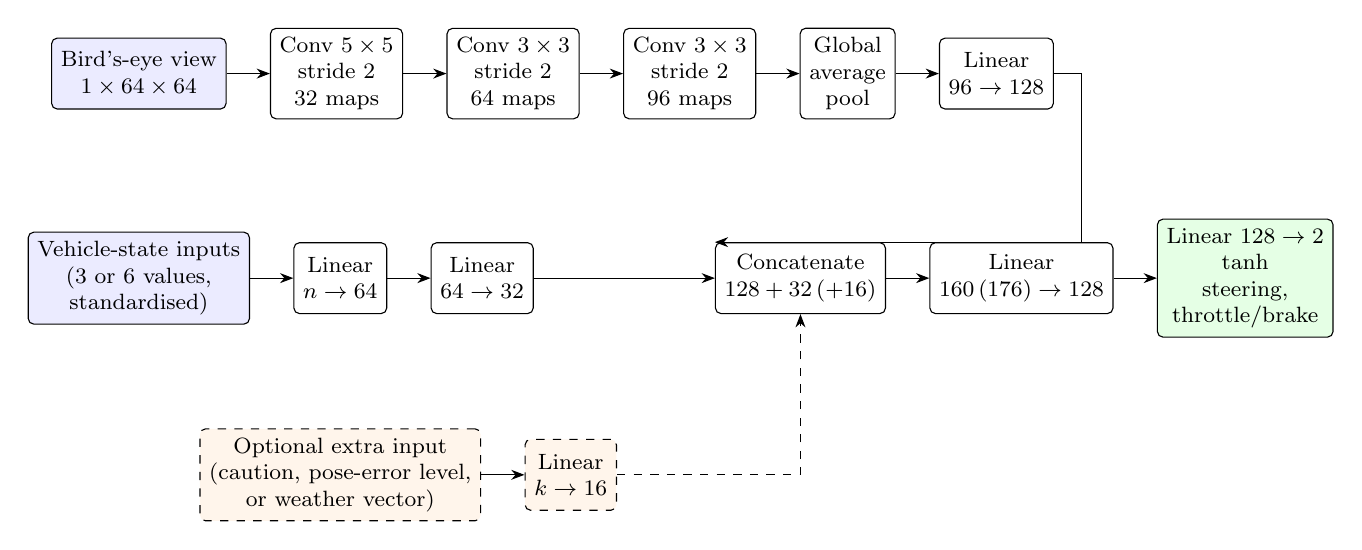
\begin{tikzpicture}[font=\footnotesize,>=Stealth,
  box/.style={draw,rounded corners=2pt,minimum height=0.9cm,align=center,fill=white},
  inbox/.style={box,fill=blue!8},
  optbox/.style={box,dashed,fill=orange!8},
  outbox/.style={box,fill=green!10},
  node distance=0.45cm and 0.55cm]
\node[inbox] (bev) {Bird's-eye view\\ $1\times64\times64$};
\node[box,right=of bev] (c1) {Conv $5\times5$\\ stride 2\\ 32 maps};
\node[box,right=of c1] (c2) {Conv $3\times3$\\ stride 2\\ 64 maps};
\node[box,right=of c2] (c3) {Conv $3\times3$\\ stride 2\\ 96 maps};
\node[box,right=of c3] (gp) {Global\\ average\\ pool};
\node[box,right=of gp] (l1) {Linear\\ $96\to128$};
\node[inbox,below=1.55cm of bev] (sc) {Vehicle-state inputs\\ (3 or 6 values,\\ standardised)};
\node[box,right=of sc] (s1) {Linear\\ $n\to64$};
\node[box,right=of s1] (s2) {Linear\\ $64\to32$};
\node[optbox,below=1.45cm of s1] (ex) {Optional extra input\\ (caution, pose-error level,\\ or weather vector)};
\node[optbox,right=of ex] (e1) {Linear\\ $k\to16$};
\node[box,right=2.3cm of s2] (cat) {Concatenate\\ $128+32\,(+16)$};
\node[box,right=of cat] (h1) {Linear\\ $160\,(176)\to128$};
\node[outbox,right=of h1] (o) {Linear $128\to2$\\ tanh\\ steering,\\ throttle/brake};
\foreach \a/\b in {bev/c1,c1/c2,c2/c3,c3/gp,gp/l1,sc/s1,s1/s2,ex/e1,cat/h1,h1/o} \draw[->] (\a) -- (\b);
\draw[->] (l1.east) -- ++(0.35,0) |- (cat.north west);
\draw[->] (s2) -- (cat);
\draw[->,dashed] (e1.east) -| (cat.south);
\end{tikzpicture}
\caption{The shared policy network. Each box is one layer; every layer except the last is followed by a rectifier. The dashed boxes exist only in the models with an extra input.
Parameter count: 110\,530 without the extra input and 112\,610 with a one-dimensional extra input.}
\label{fig:network}
\end{figure}

\paragraph{Inputs.}
\begin{description}[leftmargin=3.4cm,style=nextline]
\item[Bird's-eye view] A $64\times64$ grid covering 10\,m to each side, 17.5\,m ahead and 2.5\,m behind the car (cell size 0.3125\,m). Two encodings occur (Figure~\ref{fig:inputs}):
 \emph{unmodified} (teammates' encoding: $-1$ unknown, 0 free, 0.9 ego, 1.0 detected vehicle) and \emph{map overlay} (the reserved values 0.5 for the route centre line and 0.8 for the road boundaries are filled in from the simulator map, in the ego frame; ego and detected vehicles are never overwritten).
 Vehicles are drawn as axis-aligned blocks without heading (a limitation analysed in Section~\ref{sec:failure}).
\item[Six vehicle-state inputs] speed (m/s), route progress (fraction), lateral offset to the lane centre (m), heading error (rad), curvature ahead (rad/m), distance to the goal (m); standardised with the mean and standard deviation stored in the checkpoint.
\item[Three vehicle-state inputs] The proposed design keeps only speed, route progress and distance to goal; lateral offset, heading error and curvature are \emph{not} given as numbers because the overlay already shows the road geometry relative to the car (idea borrowed from the reinforcement-learning coach of Zhang et al., 2021).
\item[Extra input] One to four additional values through the optional 16-unit branch: the caution value $c\in[0,1]$, the pose-error level(s), or a weather vector (one-hot clear/fog/rain plus intensity).
\end{description}

\explainedfigure{fig_birds_eye_view_input_examples}{0.9}{The two input encodings of the bird's-eye-view grid, drawn from one real scenario}{The model's input is a 64 by 64 grid covering 10 metres to each side, 17.5 metres ahead and 2.5 metres behind the car. Left: the teammates' encoding (unknown, free, the ego car and detected vehicles). Right: the same grid with the route centre line and road boundaries from the map added. Both are drawn from scenario seed 5169 at step 238, with the same vehicle in view.}{In the left grid the car sees free space and a vehicle ahead but nothing about the road. In the right grid it also sees where the lane edges and the planned route are.}{The map overlay gives the model the road geometry directly, which is why three vehicle-state numbers (lateral offset, heading error, curvature) could be removed from its numeric inputs. It also creates the dependence on an accurate position estimate studied above.}{fig:inputs}


\paragraph{Output.} Two numbers in $[-1,1]$ (tanh): steering, and throttle (positive) or brake (negative), the MetaDrive action contract.

\subsection{The actor--critic variant for reinforcement learning}
For reinforcement learning (\pth{bev_rl/policy.py}, class \code{BEVActorCritic}) the network above becomes the mean of a Gaussian actor: the actor's feature extractor and head are \emph{exactly} the behaviour-cloned modules, so that at initialisation the action mean equals the imitation policy's action for every input (verified in \pth{tests/test_bev_rl_policy.py}).
A state-independent learnable log standard deviation is added (initial value $-2$, i.e.\ standard deviation 0.135), and a separate critic with its own encoder (also initialised from the cloned encoder weights, so that value-loss gradients cannot disturb the actor's features) and a randomly initialised value head.

\subsection{The Image-Only Driving Model}
For the control experiment (image-only model, \pth{bev_rl/adaptive/vanilla_camera_cnn.py}) the input is only the front-left camera image (rendered at 320$\times$240, resized to 128$\times$96, scaled to $[0,1]$), processed by five convolution layers with batch normalisation (24, 36, 48, 64, 64 maps; kernels 5, 5, 3, 3, 3, all stride 2; output $64\times3\times4$) and a multilayer perceptron head with tanh output.
It receives \emph{no} bird's-eye view, speed or weather information.

\subsection{Rule-based teachers (not learned)}\label{sec:teachers}
\begin{description}[leftmargin=3.4cm,style=nextline]
\item[Stock intelligent driver model] MetaDrive's \code{IDMPolicy}: lane keeping with same-lane car following, lane changes enabled, target speed about 30\,km/h. It sees exact simulator state. It reacts only to the vehicle ahead in its own lane.
\item[Collision-aware teacher] \codename{safe_teacher} (\pth{bev_rl/adaptive/safe_teacher.py}). The stock model with lane changes \emph{disabled} plus a privileged predictive braking layer: every other vehicle within 45\,m is predicted with a constant-velocity model over a 3\,s horizon;
 if the ego rectangle (moving with its current velocity) would overlap the other vehicle's rectangle (margins 0.35\,m laterally, 1.0\,m longitudinally) at time-to-collision $t$, the throttle command is set to full brake when $t<1.3$\,s, and to a graded brake when $1.3\le t<2.4$\,s.
 It was introduced because the stock model crashes in 45\% of dense-traffic episodes, almost always into vehicles that merge, cut in or cross from the side, which a same-lane controller never reacts to (Section~\ref{sec:failure}).
\end{description}
Both teachers use information the students do not have (exact positions and velocities of all vehicles up to 45\,m, while the student's grid ends 17.5\,m ahead); this \emph{information gap} is one of the findings of the failure analysis.

\section{Training strategies}\label{sec:training}

\begin{plainwords}
There are three ways to teach a driver in this project. (1) \emph{Copy a few recordings} of a good driver (behaviour cloning). (2) \emph{Let the driver drive, and ask a teacher what it should have done} in the situations it actually reached (dataset aggregation). (3) \emph{Trial and error with a score} (reinforcement learning). This section describes the first two in detail; the third has its own section.
\end{plainwords}
\begin{cautionbox}[Compared with GitHub]
GitHub contains only the first way: the collection script and the training script for behaviour cloning (\pth{bev_policy/collect_demos.py}, \pth{train_bc.py}), and the two checkpoints trained from five demonstrations each. Dataset aggregation, both teachers' use as labellers, the caution, position-error and degraded-perception variants, and all reinforcement learning exist only locally (Section~\ref{sec:github}).
\end{cautionbox}


\subsection{Behaviour cloning (the teammates' baselines)}
Procedure (\pth{bev_policy/collect_demos.py}, \pth{train_bc.py}): the rule-based driver (stock intelligent driver model) drives a small number of episodes; at every step the observation (grid and six vehicle-state inputs from the teammates' perception chain) and the driver's action are stored.
Only episodes that reach the destination are kept (arrival filter). The network is trained by regression on the action (mean squared error), 60 epochs maximum, batch size 64, learning rate $3\cdot10^{-4}$, early stopping with patience 10.
The two repository baselines use \textbf{five demonstrations each}: one set without other vehicles, one with sparse traffic.

\textbf{Why this is weak.} The network is trained only on states that the expert visits. Once the learner makes a small error it reaches states the expert never visited and has no labelled example of how to recover (covariate shift; Ross et al., 2011).
A concrete symptom was documented early: the cloned policy creeps to 0.8--0.96\,m from the lane centre by step 80--100 (1.58\,m for seed 1001), a systematic lateral bias. With only five demonstrations the policy also never sees most traffic situations.

\subsection{Dataset aggregation (the main training strategy)}
Dataset aggregation fixes the covariate shift by letting the \emph{learner} choose which states are visited and asking the \emph{teacher} what it would have done there. Implementation: \pth{bev_rl/adaptive/dagger_base.py} (and the variants listed below).

\begin{lstlisting}[caption={Dataset aggregation as implemented (training seeds 2000--2999, validation seeds 3100--3109).},label={lst:dagger}]
data = empty;  student = fresh network (random initialisation)
for round t = 0 .. 5:
    beta = 1.0 if t == 0 else 0.5 ** t          # probability that the TEACHER's action is executed
    for each traffic density d in {0, 0.05, 0.1, 0.2, 0.3}:
        run 8 episodes on randomly drawn training seeds:
            at every step:  record (grid, vehicle-state inputs, teacher_action)      # teacher sees the true state
                            execute teacher_action with probability beta, else student_action
                            add Gaussian noise (std 0.1) to the executed action   # widen the visited states
    data = data + new records
    student = train(student, data):  Adam, learning rate 1e-3, batch 128, mean squared error,
                                     8 epochs (24 epochs in round 0), on ALL data so far
    validate: 10 episodes (seeds 3100-3109) at densities 0.05 and 0.2, no teacher
    keep as 'best' the round with the highest mean success (ties: fewer collisions + off-road)
\end{lstlisting}
The aggregated data set holds about 67\,000 labelled steps after round 5 for the unmodified-grid student and 73\,032 for the proposed model. One training seed per model was run (seed 0); differences between rounds and between models of 0.1 in validation success correspond to a single episode of ten and must not be over-read (see Figure~\ref{fig:dagger}).

Three properties matter for interpreting the results:
\begin{itemize}
\item The teacher is a \emph{rule-based} controller that sees the exact simulator state; the student only sees the grid and a few vehicle-state inputs. The student can therefore at best match the teacher, and wherever the information is not in the student's input (for example a vehicle 30\,m away) it cannot imitate the teacher's reaction (Section~\ref{sec:failure}).
\item Model selection uses only validation seeds; the test seeds (1000--1049, 5000--5199) are never touched during training or selection.
\item In round 0 the teacher drives ($\beta=1$) and the student learns from the teacher's own distribution; the later rounds are what supply recovery behaviour.
\end{itemize}

\explainedfigure{fig_dataset_aggregation_validation_curves}{0.97}{Validation success after each training round for five input designs}{During training the model drives validation scenarios after each round (round 0: the teacher drives and the model learns from it; later rounds: the model drives and the teacher labels). Left: sparse traffic; right: dense traffic. Five designs of the model input are compared; 10 validation episodes per point.}{In sparse traffic all designs except the map overlay without vehicle-state inputs are at a validation success of 1.0 in almost every round, so this validation cannot tell them apart. In dense traffic all values are between 0 and 0.5 and differ by at most five episodes out of ten. Only the design with the map overlay but no vehicle-state inputs is clearly worse.}{A validation set of 10 episodes is too small to choose between designs, and several models ended up being the round-0 model by tie-breaking. All claims between designs therefore rest on the later 200-episode test, not on these curves.}{fig:dagger}


\subsection{Variants of the dataset-aggregation recipe}
All variants keep the optimiser, loss, action noise and network; they change one thing at a time.
\begin{table}[H]\centering\small
\caption{Variants of the dataset-aggregation recipe. ``Teacher'' is the source of labels; ``perception'' is what the student sees.}\label{tab:variants}
\begin{tabularx}{\textwidth}{@{}>{\raggedright\arraybackslash}p{3.7cm}>{\raggedright\arraybackslash}p{3.6cm}>{\raggedright\arraybackslash}p{2.8cm}X@{}}\toprule
Variant & Perception & Teacher & Specific settings\\\midrule
Input ablations & Ideal detector; unmodified or overlay grid; all, no or a subset of vehicle-state inputs (inputs hidden by constants) & Stock model & Densities 0--0.3; validation densities 0.05 and 0.2.\\
Proposed model & Ideal detector; overlay grid; vehicle-state inputs speed, progress, goal & Stock model & As above.\\
Safe-teacher student & As the proposed model & Collision-aware teacher & Densities 0, 0.05, 0.1; validation 0.05; 7 rounds (0--6).\\
Caution study caution-study caution-aware model, caution-study control model & Detector dropout at measured retention per weather; overlay grid & Caution-aware stock model (caution 0: 30\,km/h, 10\,m gap; caution 1: 20\,km/h, 25\,m gap) & Caution value per episode: half uniform in $[0,1]$, half derived from weather as $1-\text{retention}$; control network has the input fixed to 0.\\
Degraded-perception student weather-degradation-trained model & Calibrated degradation (missed detections and range errors, Section~\ref{sec:perception}); overlay grid & Collision-aware teacher on ground truth & Training weather mix: clear (twice), fog 0.8 and 1.0, rain 0.3, 0.6, 1.0 (twice); densities 0.05, 0.05, 0.1, 0; 5 rounds; 6 epochs.\\
Pose-error students & Ideal detector; overlay drawn from a \emph{wrong} car pose & Stock model on the true state & Per episode an error level $L$ ($30\%$ exactly 0, 70\% uniform): lateral error $\pm1.5L$\,m, heading error $\pm0.15L$\,rad; conditioned variants receive $L$; two-cue variants additionally receive noisy lateral and heading vehicle-state inputs.\\
Image-Only Driving Model & Front-camera image & Collision-aware teacher & Behaviour cloning on clean images with action noise (0, 0.1, 0.25), then three dataset-aggregation rounds.\\\bottomrule
\end{tabularx}
\end{table}

\subsection{Reinforcement learning}
Four reinforcement-learning attempts are described in Section~\ref{sec:rl}. Common to all of them is the algorithm (proximal policy optimisation from Stable-Baselines3: 256 steps per update per environment, batch 128, 5 epochs, discount 0.99, GAE parameter 0.95, clip range 0.1, no entropy bonus, target KL 0.02; the first attempt used a plain multilayer-perceptron policy with 512 steps per update, batch 512, 10 epochs, clip range 0.2 and target KL 0.03),
and the idea of starting from an imitation-trained network instead of from random weights, because a random start settles in a stand-still optimum (zero speed is the safest behaviour).

\section{Model catalogue}\label{sec:catalogue}

\begin{plainwords}
Thirty-three model files were saved. This section names every one, says what goes into it, who labelled its training data, how it was trained, and where it was evaluated. The model names used everywhere in this report are the descriptive names in the first column. The \emph{internal nickname} in the second column is how the model appears in old logs, result files and run folders; it is given once, here, so that nothing has to be decoded. The file name of every model and its hash are in Appendix~\ref{app:inventory}, and the mapping from the previous to the current file names is in \pth{trained_models/MODEL_NAME_MAPPING.md}.
\end{plainwords}

\paragraph{How to read the ``selected round'' column.} Training proceeds in rounds (Section~\ref{sec:training}); the round whose model is kept is the one with the highest validation success, and \emph{ties keep the earliest round}. Because validation uses only ten episodes and reaches 1.0 in sparse traffic, ties are frequent, and in four runs the kept model is round 0, in which the teacher drives and the model is simply behaviour-cloned from the teacher's own demonstrations. These are marked \textbf{round 0}.

{\small
\begin{longtable}{@{}>{\raggedright\arraybackslash}p{3.7cm}>{\raggedright\arraybackslash}p{1.9cm}>{\raggedright\arraybackslash}p{3.0cm}>{\raggedright\arraybackslash}p{2.3cm}>{\raggedright\arraybackslash}p{2.0cm}>{\raggedright\arraybackslash}p{1.9cm}@{}}
\caption{Catalogue of the trained models. ``GitHub'' states whether the checkpoint is committed on the GitHub repository (only the two baseline models are).}\label{tab:catalogue}\\
\toprule Descriptive name & Internal nickname & Input & Labels & Selected round; data & GitHub; evidence\\\midrule\endfirsthead
\toprule Descriptive name & Internal nickname & Input & Labels & Selected round; data & GitHub; evidence\\\midrule\endhead
\midrule\multicolumn{6}{r}{\emph{continued on the next page}}\\\endfoot
\bottomrule\endlastfoot
\multicolumn{6}{@{}l}{\textbf{A. Baseline models supplied by the teammates}}\\
Baseline Driving Model Trained Without Traffic & repo\_bc\_clear & Plain grid; six vehicle-state inputs & Stock driver model; 5 episodes, no other vehicles & Supervised only & \textbf{Yes}; 200 episodes: 0.850\\
Baseline Driving Model Trained With Traffic & repo\_bc\_sparse & Plain grid; six vehicle-state inputs & Stock driver model; 5 episodes, traffic 0.05 & Supervised only & \textbf{Yes}; 200 episodes: 0.745\\
\multicolumn{6}{@{}l}{\textbf{B. Imitation-trained models (dataset aggregation)}}\\
\textbf{Proposed Bird's-Eye-View Driving Model} & ov\_split & Map-overlay grid; speed, route progress, distance to goal & Stock driver model & Round 5; 73\,032 samples; validation 1.0 sparse, 0.5 dense & No; \textbf{200 episodes: 0.925}\\
Ablation: Plain BEV With Six State Inputs & base\_a & Plain grid; six vehicle-state inputs & Stock driver model & Round 5; 66\,956; 1.0 / 0.4 & No; 10 and 40 episodes\\
Ablation: Map-Overlay BEV With Six State Inputs & ov\_both & Map-overlay grid; six inputs & Stock driver model & Round 5; 71\,642; 1.0 / 0.5 & No; 10 episodes\\
Ablation: Map-Overlay BEV Without State Inputs & ov\_bev\_only & Map-overlay grid only & Stock driver model & Round 4; 60\,590; 0.5 / 0.2 & No; 10 episodes (worst)\\
Ablation: Plain BEV Without State Inputs & arch\_bev\_only & Plain grid only & Stock driver model & \textbf{Round 0}; 11\,388; 0.0 / 0.0 & No; not evaluated further\\
Ablation: Six State Inputs Without BEV & arch\_scalar\_only & Six vehicle-state inputs only & Stock driver model & \textbf{Round 0}; 11\,388; 1.0 / 0.3 & No; 10 episodes\\
Proposed BEV Model Trained From the Collision-Aware Teacher & sparse\_overlay\_ split\_safe\_ teacher & As the proposed model & Collision-aware teacher & \textbf{Round 0}; 18\,824; 1.0 (sparse) & No; \emph{not evaluated on 200 episodes}\\
Weather-Degradation-Trained Driving Model & deg\_base & Map-overlay grid under measured degradation; three vehicle-state inputs & Collision-aware teacher & Round 5; 104\,292; validation 0.933 & No; 200 episodes in four weather conditions\\
C. Caution study & & & & &\\
\quad Caution-Study Caution-Aware Driving Model & caut\_a & As proposed + caution input & Caution-aware stock model & Round 1; 35\,503 & No; 40 episodes\\
\quad Caution-Study Control Model (caution input fixed to zero) & ctrl\_nocaut & As proposed + input fixed 0 & Caution-aware stock model & \textbf{Round 0}; 16\,835 & No; 200 episodes: 0.895\\
D. Position-error study (four models) & pose\_aug\_*, pose\_cam\_* & Map overlay drawn from a wrong position; two variants with a second noisy lane cue; two with the error level as input & Stock model on the true state & Rounds 2 to 4; 56\,646 to 96\,706 & No; 40 episodes\\
\multicolumn{6}{@{}l}{\textbf{E. Reinforcement-learning models (Section~\ref{sec:rl})}}\\
Reinforcement Learning Attempt 1: privileged teachers (runs C2, Probe C, C3) and their initialisation & C2, probe\_C, C3, bc\_init & Simulator state (12 numbers) & Reward version 1 & 1.5, 1 and 0.3 million steps & No; 70 episodes\\
Reinforcement Learning Attempt 2: Fine-Tuned Proposed Model With Weather Input & pilot\_cond & Proposed model + weather input & Reward version 1 & 120\,000 steps & No; validation only\\
Reinforcement Learning Attempt 3: Reward Sweep (five models) & rl\_plain, rl\_energy, rl\_safe, rl\_head, rl\_full & Proposed model + caution input & Five reward combinations & 150\,000 steps each & No; validation only\\
Reinforcement Learning Attempt 4: Fine-Tuned Without Weather Input & ppo\_plain & As the weather-degradation-trained model & Reward version 3 & 300\,000 steps & No; 200 episodes in four weather conditions\\
Reinforcement Learning Attempt 4: With Weather Input (INCOMPLETE, untrained) & ppo\_ada & As above + weather input & Reward version 3 & Step 0 only & No; unusable\\
\multicolumn{6}{@{}l}{\textbf{F. Image-only model and third-party weights}}\\
Image-Only Driving Model (Front Camera) & vcam & Front-camera picture (128 by 96 pixels) & Collision-aware teacher & Behaviour cloning on 40 episodes, then three dataset-aggregation rounds & No; \textbf{200 episodes} (Section~\ref{sec:headline})\\
YOLO Version 8 Nano Object Detector Weights (third party) & yolov8n & Camera image & Pretrained by Ultralytics & Not trained here & No (local copy)\\
\multicolumn{6}{@{}l}{\textbf{G. Superseded early experiment (not used for results)}}\\
Early Camera-View Version 2 Models (three) & bcv2\_* & Seven-channel camera view; six inputs; with or without weather input & Stock driver model; 40 episodes, no traffic & Supervised only & No; open-loop only\\
\end{longtable}
}

\subsection{What each family is for}
\begin{description}[leftmargin=0.4cm,style=nextline]
\item[Baseline models (A).] The comparison points supplied with the project; the README recommends the traffic-trained one as the starting point for reinforcement learning.
\item[Imitation-trained models (B).] Five input designs (the proposed model and four ablations) isolate where the proposed model's performance comes from: moving the lane geometry out of the numeric inputs and into the map overlay, or removing either input entirely. The collision-aware-teacher variant and the weather-degradation-trained model test the teacher and the perception conditions.
\item[Caution study (C).] Tests the idea that a driver should become more careful when its perception is less reliable: a ``caution'' input derived from measured detector retention, a teacher whose speed and gap depend on it, and a control with identical data and network but the input fixed at zero.
\item[Position-error study (D).] Tests robustness to an error in the car's own position against the map, a realistic failure of map-based localisation.
\item[Reinforcement-learning models (E).] Section~\ref{sec:rl}.
\item[Image-only model (F).] A control: it reads the camera picture itself instead of the grid, and shows what the grid representation contributes.
\end{description}

\section{Main result: 200 paired episodes in clear weather}\label{sec:headline}

\begin{plainwords}
Seven drivers (and two rule-based teachers) drove the same 200 scenarios. The driver we propose succeeds in 92.5\% of them. The two baseline drivers that are committed on GitHub succeed in 85.0\% and 74.5\%. The proposed driver is statistically as good as the teacher it learned from.
\end{plainwords}
\begin{cautionbox}[Compared with GitHub]
The GitHub README states 90\% success (9 of 10 episodes) for the traffic-trained baseline. On 200 episodes the same checkpoint scores 74.5\% (interval 0.680 to 0.800); the README figure comes from ten episodes with the full camera pipeline, whose interval (0.60 to 0.98) is compatible with it. Table~\ref{tab:githubbaseline} gives the comparison.
\end{cautionbox}


\paragraph{Protocol.} Seeds 5000--5199, sparse traffic (density 0.05), clear weather, horizon 800 steps; the same 200 scenarios for every model; script \pth{bev_rl/adaptive/evaluate_final_200seed_sparse.py}; per-episode results in \pth{bev_rl/adaptive/results/final_200seed/}.
No model was trained, validated or selected on these seeds. Six models are compared: the two rule-based teachers (which see the exact simulator state), the proposed model, the caution-study control, and the two behaviour-cloning baselines.

\explainedfigure{fig_headline_success_clear_weather_200_episodes}{0.97}{Success rate of the driving models on the same 200 test episodes}{Each bar is the share of 200 identical test episodes (scenario seeds 5000 to 5199, clear weather, sparse traffic) in which a model reached the destination without a collision and without leaving the road. The black line is the 95\% Wilson confidence interval, the range of success rates that is statistically compatible with the observed count. Grey bars are rule-based teachers that see the exact simulator state; orange bars are the two baseline models supplied by the teammates; blue bars are models trained in this project.}{The Proposed Bird's-Eye-View Driving Model succeeds in 92.5\% of the episodes. The two baseline models succeed in 85.0\% (trained without traffic) and 74.5\% (trained with traffic). The proposed model is about as good as the Collision-Aware Teacher (95.0\%) whose behaviour it learned; the intervals overlap, so the two cannot be told apart. The Image-Only Driving Model, which reads camera pixels instead of the bird's-eye-view grid, reaches 0.130 (interval 0.090 to 0.184), far below every model that uses the grid.}{Training a model by letting it drive and asking a teacher what it should have done (dataset aggregation) produces a model that matches its teacher and clearly beats few-demonstration behaviour cloning. This figure does not say \emph{which part} of the proposed design (the training method or the map overlay) causes the gain; that needs the additional evaluations listed in the paper-directions section.}{fig:headline}


\begin{table}[H]\centering\small
\caption{Result table for the 200 clear-weather episodes (95\% Wilson intervals; ``Left road'' includes leaving the planned route; energy is the estimate of Section~\ref{sec:setup}).}\label{tab:headline}
\resizebox{\textwidth}{!}{\begin{tabular}{@{}lrrrrrrr@{}}\toprule
Model & Success & 95\% interval & Collision & Left road & Timeout & Speed (m/s) & Energy (Wh per km)\\\midrule
Collision-Aware Teacher (rule-based; sees exact simulator state) & 0.950 & [0.910, 0.973] & 0.010 & 0.040 & 0.000 & 7.84 & 101.3\\
Proposed Bird's-Eye-View Driving Model (map overlay + 3 vehicle-state inputs) & 0.925 & [0.880, 0.954] & 0.060 & 0.010 & 0.005 & 7.87 & 96.2\\
Caution-Study Control Model (caution input fixed to zero) & 0.895 & [0.845, 0.930] & 0.105 & 0.000 & 0.000 & 7.98 & 80.4\\
Stock Intelligent Driver Model (rule-based; sees exact simulator state) & 0.885 & [0.833, 0.922] & 0.080 & 0.035 & 0.000 & 7.90 & 97.9\\
Baseline Driving Model Trained Without Traffic & 0.850 & [0.794, 0.893] & 0.125 & 0.025 & 0.000 & 8.09 & 85.9\\
Baseline Driving Model Trained With Traffic & 0.745 & [0.680, 0.800] & 0.120 & 0.135 & 0.000 & 8.07 & 90.7\\
Image-Only Driving Model (reads front-camera pixels) & 0.130 & [0.090, 0.184] & 0.200 & 0.605 & 0.065 & 9.20 & 276.6\\
\bottomrule\end{tabular}
}
\end{table}

\subsection{The Image-Only Driving Model on the same 200 episodes}
The Image-Only Driving Model (front-camera picture of 128 by 96 pixels as its only input; Section~\ref{sec:arch}) was evaluated on the same 200 scenarios with the same metrics (script \pth{bev_rl/adaptive/vanilla_camera_cnn.py eval}; per-episode results in \pth{bev_rl/adaptive/results/vanilla_camera/}). It differs from the other models in the harness only in what it reads: it is driven by a rendered 320 by 240 camera image instead of the grid, so no detector or degradation model is involved (clear weather).
Result: success \ImOnSuccess{} (95\% interval \ImOnLow{} to \ImOnHigh{}); collisions \ImOnCollision{}, left the road \ImOnOffroad{}, timeouts \ImOnTimeout{}; mean speed \ImOnSpeed{} metres per second; estimated energy \ImOnEnergy{} watt-hours per kilometre. It is included in the figures and tables of this section.
\begin{implicationbox}
A driver that reads the picture directly is far below every driver that reads the grid. The grid is a compact, structured summary produced by the object detector and the stereo depth; with the amount of training here, a network cannot recover that summary from raw pixels. Whether more data would close the gap is not tested.
\end{implicationbox}

\subsection{What the numbers say}
\begin{itemize}
\item \textbf{The proposed model is clearly better than both baselines.} 0.925 against 0.850 (no-traffic baseline) and 0.745 (sparse-traffic baseline). The paired differences are $+0.075$ (95\% interval $[+0.035,+0.120]$, exact McNemar $p=0.0007$) and $+0.180$ ($[+0.125,+0.240]$, $p<0.0001$); see Figure~\ref{fig:paired} and Table~\ref{tab:paired}.
  The baselines' failures are of a different kind: the sparse-traffic baseline leaves the road in 13.5\% of the episodes (proposed model: 1.0\%), a sign of lateral drift, and the no-traffic baseline collides in 12.5\%.
\item \textbf{The proposed model is statistically indistinguishable from the collision-aware teacher} it is trained to imitate (difference $-0.025$, interval $[-0.070,+0.020]$, $p=0.40$), and $+0.040$ better than the stock driver model (interval $[0.000,+0.080]$, $p=0.077$, i.e.\ not significant at the 5\% level).
\item \textbf{The caution-study control (0.895) is not significantly different from the proposed model} ($+0.030$, $p=0.18$). Its apparent 0.975 on 40 episodes (Section~\ref{sec:weather}) was a selection effect of a small sample: the best of several candidates evaluated on 40 episodes regresses towards its true value when re-evaluated on 200.
\item \textbf{Energy.} The proposed model uses an estimated 96.2\,watt-hours per kilometre at 7.87\,m/s, similar to the stock driver model (97.9\,watt-hours per kilometre) and the collision-aware teacher (101.3). The two behaviour-cloning baselines use less (85.9 and 90.7\,watt-hours per kilometre) \emph{and drive faster} (8.09 and 8.07\,m/s) because they are less careful. The caution-study control is the cheapest model (80.4\,watt-hours per kilometre) at 7.98\,m/s with 89.5\% success;
  the reason for its lower consumption has not been investigated (Figure~\ref{fig:energy}).
\end{itemize}

\explainedfigure{fig_outcome_breakdown_200_episodes}{0.97}{How the 200 test episodes end, for each model}{For every model, the 200 episodes are split into the four possible outcomes: success (green), collision (red), left the road (yellow) and timeout (grey). Each bar sums to one.}{The proposed model fails almost only by collision (6.0\% collisions, 1.0\% left the road, 0.5\% timeouts). The baseline trained with traffic leaves the road in 13.5\% of the episodes and collides in 12.0\%; the baseline trained without traffic collides in 12.5\%. The Image-Only Driving Model ends 0.200 of the episodes in a collision, 0.605 by leaving the road and 0.065 by timeout.}{The baselines fail in a way that points to \emph{drift}: with only five demonstrations they never saw how to recover from a small steering error, so they slide off the road. Iterative training removes that failure type (1.0\% left the road). What remains for the proposed model is collisions with other vehicles, which points to what the model can see rather than to how it was trained.}{fig:outcomes}


\explainedfigure{fig_paired_difference_headline_versus_others}{0.97}{Paired difference in success between the proposed model and each other model}{For each comparison the difference (proposed model minus the other model) is computed on the same 200 episodes. The point is the difference; the black line is the 95\% bootstrap interval obtained by resampling episodes 5000 times. A line entirely to the right of the zero line means the proposed model is better with statistical support.}{The proposed model is better than the baseline trained without traffic by 0.075 (interval $+0.035$ to $+0.120$) and better than the baseline trained with traffic by 0.180 (interval $+0.125$ to $+0.240$). Its differences to the Collision-Aware Teacher ($-0.025$), the caution-study control ($+0.030$) and the stock driver model ($+0.040$) have intervals that include or touch zero. The Image-Only Driving Model is far below it.}{The claim that the proposed model beats the two baselines is statistically supported. No claim is made that it beats the teachers or the control. Using paired comparisons (same scenarios for every model) is what makes a difference of 0.075 detectable with 200 episodes.}{fig:paired}


\begin{table}[H]\centering\small
\caption{Paired comparison of the proposed model with each other model. ``Only proposed model'' counts the seeds on which the proposed model succeeded and the other model did not; the exact McNemar test uses only these discordant seeds.}\label{tab:paired}
\resizebox{\textwidth}{!}{\begin{tabular}{lrrrrr}\toprule
Compared model & Difference & 95\% interval & Only proposed model succeeded & Only compared model succeeded & Exact McNemar $p$ \\\midrule
Collision-Aware Teacher & -0.025 & [-0.075, +0.020] & 9 & 14 & 0.4049 \\
Caution-Study Control Model & +0.030 & [-0.005, +0.065] & 10 & 4 & 0.1796 \\
Stock Intelligent Driver Model & +0.040 & [+0.000, +0.080] & 12 & 4 & 0.0768 \\
Baseline Driving Model Trained Without Traffic & +0.075 & [+0.035, +0.120] & 17 & 2 & 0.0007 \\
Baseline Driving Model Trained With Traffic & +0.180 & [+0.125, +0.240] & 38 & 2 & $<0.0001$ \\
Image-Only Driving Model & +0.795 & [+0.740, +0.850] & 159 & 0 & $<0.0001$ \\
\bottomrule\end{tabular}
}
\end{table}

\explainedfigure{fig_per_episode_outcome_strips}{0.97}{Which test episodes each model fails}{Each thin column is one of the 200 test episodes; each row is one model. Green means the model succeeded in that episode, red means it failed. The episodes are sorted so that those failed by no model are on the left and those failed by many models are on the right.}{Most episodes are solved by every model. The failures are concentrated in a small set of hard scenarios on the right, and the models fail many of the same ones. The two baselines also fail a block of episodes that all the other models solve.}{Because failures cluster in particular scenarios, the remaining errors can be studied scenario by scenario instead of treated as random. This is what the failure analysis does, and it is why the comparison is paired (all models see the same scenarios).}{fig:strips}


\explainedfigure{fig_speed_versus_energy_200_episodes}{0.97}{Mean driving speed and estimated energy use of each model}{Each point is one model, placed by its mean speed (horizontal, metres per second) and its estimated traction energy per kilometre (vertical, watt-hours per kilometre) over the 200 clear-weather test episodes. The energy value is the mechanical work at the wheels of a declared virtual vehicle (no regenerative braking), not a battery measurement.}{The two baselines use less energy (85.9 and 90.7 watt-hours per kilometre) and drive faster (8.09 and 8.07 metres per second) than the proposed model (96.2 watt-hours per kilometre at 7.87 metres per second), because they are less careful. The caution-study control is the cheapest (80.4 watt-hours per kilometre).}{Energy comparisons are only meaningful between models with similar safety; a model that crashes early also uses little energy. Differences are valid as comparisons between models, not as absolute battery figures.}{fig:energy}


\subsection{What this result does \emph{not} show}
\begin{itemize}
\item It does not separate the \emph{causes} of the proposed model's gain over the baselines. Three things changed at once relative to the baseline behaviour cloning: (i) dataset aggregation instead of five demonstrations (the main suspect), (ii) the map overlay in the grid, (iii) the split of the vehicle-state inputs. A student with the unmodified grid and all six vehicle-state inputs was evaluated on 10 and 40 episodes only (0.70/0.875, not significantly different from the proposed model's 0.80/0.925);
  \textbf{it has not been evaluated on the 200-episode block}, so the contribution of the overlay at this sample size is untested (Section~\ref{sec:directions}).
\item It does not show anything about dense traffic: no learned model solves it (Section~\ref{sec:failure}).
\item It is a result of the camera-free surrogate (Section~\ref{sec:surrogate}), not of the live camera pipeline.
\end{itemize}

\section{Weather, caution, input design and robustness to pose error}\label{sec:weather}

\begin{plainwords}
This section answers the original question: does the driving get worse in fog and rain? The answer is no, in sparse traffic, for the perception damage we measured. It also reports three side studies: a driver that becomes cautious when its perception is unreliable, which input design works best, and what happens when the car's position estimate on the map is wrong.
\end{plainwords}
\begin{cautionbox}[Compared with GitHub]
The GitHub README lists the weather evaluation as ``preliminary tooling'' and states that it ``does not change vehicle dynamics or road friction'' and is ``not evidence of physical fog/rain robustness or adaptive driving''. The results below complete that picture within the same limits: weather acts only through the camera pipeline and, in this report, only through a measured degradation of what the model sees.
\end{cautionbox}


This section contains the results that bear on the original question (``can the policy keep driving, and drive more economically, when its perception degrades?''), in the order in which the evidence was produced.

\subsection{Detector-dropout proxy: no effect (pilot, 40 episodes)}
With the dropout proxy (each vehicle removed from the grid with the measured retention probability of the weather), three models were evaluated on seeds 1010--1049 (Table~\ref{tab:dropout}). The success rates are \emph{identical} across weather conditions for the unmodified-grid student and differ by at most one episode (0.025) for the other two models. Even at rain 1.0, where only 4\% of the vehicles survive, nothing changes.
\begin{table}[H]\centering\small
\caption{Success under the detector-dropout proxy, sparse traffic, seeds 1010--1049 (pilot; 40 episodes per cell). ``Share of vehicles kept'' is the measured detector retention used by the proxy.}\label{tab:dropout}
\resizebox{\textwidth}{!}{\begin{tabular}{@{}llrrr@{}}\toprule
Model & Weather & Share of vehicles kept & Success (40 episodes) & 95\% interval\\\midrule
Baseline behaviour cloning, sparse-traffic demonstrations & clear & 1.00 & 0.775 & [0.62, 0.88]\\
 & fog 1.0 & 0.27 & 0.800 & [0.65, 0.90]\\
 & rain 0.6 & 0.16 & 0.800 & [0.65, 0.90]\\
 & rain 1.0 & 0.04 & 0.800 & [0.65, 0.90]\\
Baseline behaviour cloning, no-traffic demonstrations & clear & 1.00 & 0.875 & [0.74, 0.95]\\
 & fog 1.0 & 0.27 & 0.875 & [0.74, 0.95]\\
 & rain 0.6 & 0.16 & 0.875 & [0.74, 0.95]\\
 & rain 1.0 & 0.04 & 0.875 & [0.74, 0.95]\\
Dataset-aggregation student, unmodified view & clear & 1.00 & 0.875 & [0.74, 0.95]\\
 & fog 1.0 & 0.27 & 0.875 & [0.74, 0.95]\\
 & rain 0.6 & 0.16 & 0.875 & [0.74, 0.95]\\
 & rain 1.0 & 0.04 & 0.875 & [0.74, 0.95]\\
Headline model (map-overlay view) & clear & 1.00 & 0.925 & [0.80, 0.97]\\
 & fog 1.0 & 0.27 & 0.925 & [0.80, 0.97]\\
 & rain 0.6 & 0.16 & 0.925 & [0.80, 0.97]\\
 & rain 1.0 & 0.04 & 0.950 & [0.83, 0.99]\\
\bottomrule\end{tabular}
}
\end{table}

\subsection{Calibrated degradation: no effect (reported, 200 episodes)}
After the measurement of Section~\ref{sec:perception} the environment was rebuilt so that vehicles can both disappear and be displaced by a wrong stereo range (\pth{bev_rl/adaptive/degraded_env.py}); weather conditions: clear, fog 1.0, rain 0.6, rain 1.0.
Following the pre-registration, the first test (H1) asked whether a clean-trained model gets \emph{worse} under the calibrated degradation: proposed model, 100 paired episodes, seeds 5000--5099: clear 0.89, fog 1.0: 0.90, rain 0.6: 0.89, rain 1.0: 0.89 (exact McNemar $p=1.0$ for every degraded cell against clear). \textbf{H1 failed}: the pre-registered consequence is that adaptation cannot be demonstrated on success in sparse traffic, and everything that follows is exploratory.
On 200 episodes four models give the picture of Figure~\ref{fig:weather}.

\explainedfigure{fig_success_by_weather_calibrated_perception_200_episodes}{0.97}{Success rate in four weather conditions under the measured perception degradation}{Four models were each evaluated on the same 200 episodes in clear weather, fog of intensity 1.0, rain of intensity 0.6 and rain of intensity 1.0. In every weather condition the input of the model was degraded as measured: vehicles can disappear from the bird's-eye-view grid, or be placed at a wrong distance. Black lines are 95\% intervals.}{The proposed model stays between 0.89 and 0.91 in all four conditions; the weather-degradation-trained model between 0.88 and 0.90. The reinforcement-learning-fine-tuned model is lower in every condition (0.765 to 0.815) and the baseline trained with traffic is flat at about 0.75.}{Under the perception degradation that was measured and implemented, weather does not lower driving success in sparse traffic. It follows that a robustness or weather-adaptation claim cannot be made from this experiment, and that a weather-adaptive method would have nothing to adapt to here. The next research step is to find the conditions (denser traffic, harsher loss of vehicles) under which weather begins to matter.}{fig:weather}

\begin{table}[H]\centering\small
\caption{Full numbers for Figure~\ref{fig:weather}.}\label{tab:weather}
\resizebox{\textwidth}{!}{\begin{tabular}{llrrrrrr}\toprule
Model & Weather & Success & 95\% interval & Collision & Left road & Timeout & Energy (Wh per km) \\\midrule
Proposed Bird's-Eye-View Driving Model & clear 0.0 & 0.900 & [0.851, 0.934] & 0.075 & 0.020 & 0.005 & 97.9 \\
Proposed Bird's-Eye-View Driving Model & fog 1.0 & 0.890 & [0.839, 0.926] & 0.085 & 0.020 & 0.005 & 96.2 \\
Proposed Bird's-Eye-View Driving Model & rain 0.6 & 0.905 & [0.856, 0.938] & 0.090 & 0.005 & 0.000 & 95.2 \\
Proposed Bird's-Eye-View Driving Model & rain 1.0 & 0.890 & [0.839, 0.926] & 0.105 & 0.005 & 0.000 & 91.9 \\
Weather-Degradation-Trained Driving Model & clear 0.0 & 0.880 & [0.828, 0.918] & 0.110 & 0.000 & 0.010 & 88.8 \\
Weather-Degradation-Trained Driving Model & fog 1.0 & 0.895 & [0.845, 0.930] & 0.105 & 0.000 & 0.000 & 86.8 \\
Weather-Degradation-Trained Driving Model & rain 0.6 & 0.880 & [0.828, 0.918] & 0.120 & 0.000 & 0.000 & 86.9 \\
Weather-Degradation-Trained Driving Model & rain 1.0 & 0.890 & [0.839, 0.926] & 0.110 & 0.000 & 0.000 & 86.2 \\
Reinforcement-Learning-Fine-Tuned Model & clear 0.0 & 0.815 & [0.755, 0.863] & 0.170 & 0.015 & 0.000 & 104.0 \\
Reinforcement-Learning-Fine-Tuned Model & fog 1.0 & 0.780 & [0.718, 0.832] & 0.195 & 0.025 & 0.000 & 104.2 \\
Reinforcement-Learning-Fine-Tuned Model & rain 0.6 & 0.765 & [0.702, 0.818] & 0.215 & 0.020 & 0.000 & 104.2 \\
Reinforcement-Learning-Fine-Tuned Model & rain 1.0 & 0.795 & [0.734, 0.845] & 0.200 & 0.005 & 0.000 & 103.4 \\
Baseline Driving Model Trained With Traffic & clear 0.0 & 0.750 & [0.686, 0.805] & 0.120 & 0.130 & 0.000 & 90.8 \\
Baseline Driving Model Trained With Traffic & fog 1.0 & 0.755 & [0.691, 0.809] & 0.120 & 0.125 & 0.000 & 90.5 \\
Baseline Driving Model Trained With Traffic & rain 0.6 & 0.755 & [0.691, 0.809] & 0.120 & 0.125 & 0.000 & 90.5 \\
Baseline Driving Model Trained With Traffic & rain 1.0 & 0.755 & [0.691, 0.809] & 0.120 & 0.125 & 0.000 & 90.5 \\
\bottomrule\end{tabular}
}
\end{table}

\paragraph{Pre-registered hypotheses, final status.}
\textbf{H0} (the perturbation is real): confirmed, for the detector and for stereo-depth validity (Section~\ref{sec:perception}).
\textbf{H1} (it hurts a clean-trained policy): \emph{not} confirmed.
\textbf{H2} (a weather-input policy beats its non-adaptive control): \emph{not testable}; the reinforcement-learning run with the weather input died after step 0, and the non-adaptive control got worse than its start.
\textbf{H3} (training under degradation helps): \emph{not} confirmed (the degraded-perception student 0.888 pooled over the three degraded cells against 0.895 for the proposed model).

\paragraph{Why weather does not matter here (explanations, partly tested).}
(i)~What is lost is almost only the \emph{detection} of vehicles (Section~\ref{sec:perception}); the map, the road and the car's own state are unaffected. (ii)~In sparse traffic few episodes involve a vehicle near the route in the first place; the failures that exist (Section~\ref{sec:failure}) are dominated by sudden crossings and oncoming vehicles that appear late anyway.
(iii)~Weather has no dynamics effect in this setup, so the road remains as grippy as in clear weather. Explanations (ii) and (iii) were not tested by a dedicated experiment.

\subsection{Caution coupled to perception reliability: learned adaptive behaviour (pilot at 40 episodes, confirmed at 200)}
The caution study tested whether a network that receives a caution value derived from the measured reliability of the detector ($c=1-\text{retention}$) drives more slowly and economically when perception is poor.
\begin{table}[H]\centering\small
\caption{Caution study, sparse traffic, seeds 1010--1049 (40 episodes per cell, pilot).}\label{tab:caution}
\resizebox{\textwidth}{!}{\begin{tabular}{@{}llrrrr@{}}\toprule
Model & Weather & Success & Timeout & Speed (m/s) & Energy (Wh per km)\\\midrule
Headline model & clear 0.0 & 0.925 & 0.000 & 7.94 & 93.0\\
Headline model & fog 1.0 & 0.925 & 0.000 & 7.95 & 94.3\\
Headline model & rain 0.6 & 0.900 & 0.000 & 7.95 & 93.6\\
Headline model & rain 1.0 & 0.925 & 0.000 & 7.97 & 89.4\\
Control: caution input fixed to 0 & clear 0.0 & 0.975 & 0.000 & 8.02 & 74.7\\
Control: caution input fixed to 0 & fog 1.0 & 0.975 & 0.000 & 8.02 & 74.6\\
Control: caution input fixed to 0 & rain 0.6 & 0.975 & 0.000 & 8.02 & 74.3\\
Control: caution input fixed to 0 & rain 1.0 & 0.975 & 0.000 & 8.02 & 74.5\\
Caution-conditioned network, caution 0 & clear 0.0 & 0.900 & 0.000 & 8.02 & 84.7\\
Caution-conditioned network, caution 0 & fog 1.0 & 0.900 & 0.000 & 8.02 & 84.5\\
Caution-conditioned network, caution 0 & rain 0.6 & 0.900 & 0.000 & 8.02 & 84.1\\
Caution-conditioned network, caution 0 & rain 1.0 & 0.900 & 0.000 & 8.02 & 84.3\\
Caution-conditioned network, caution from weather & clear 0.0 & 0.900 & 0.000 & 8.02 & 84.7\\
Caution-conditioned network, caution from weather & fog 1.0 & 0.925 & 0.075 & 6.17 & 59.1\\
Caution-conditioned network, caution from weather & rain 0.6 & 0.900 & 0.100 & 5.89 & 57.0\\
Caution-conditioned network, caution from weather & rain 1.0 & 0.850 & 0.150 & 5.58 & 56.1\\
\bottomrule\end{tabular}
}
\end{table}
Findings: the caution mechanism works as designed (mean speed falls from 8.0 to 5.6--6.2\,m/s and the estimated energy from 84.7 to 56--59\,watt-hours per kilometre as soon as weather is present), at the price of more timeouts (7.5--15\%, because the slower car does not always finish within 800 steps) and, at rain 1.0, a lower success (0.85).
Success is \emph{not} higher than without caution (the fixed-zero control reached 0.975 on these 40 episodes but 0.895 on 200). So the evidence shows \textbf{learned adaptive behaviour}: the student, trained by dataset aggregation from a teacher whose speed and gap depend on the caution value, reproduces that dependence on its own (it slows down in weather; the control with the input fixed at zero does not). It also shows a speed--energy trade-off. It does \emph{not} show a benefit to success: weather does not hurt the proposed model in the first place, so there was no loss for the adaptation to recover. Two limits: what caution means (30 down to 20 km/h, gap 10 up to 25 m) is defined by the teacher, and the caution value is supplied from the known weather (one minus measured detector retention), not sensed by the model from its own perception.

\subsection{Input design (pilot, 10 episodes)}
Five input designs were compared early in the project with one training seed each and 10 episodes per cell, hence wide intervals (Table~\ref{tab:ablation}).
\begin{table}[H]\centering\small
\caption{Input-design ablation, seeds 1000--1009 (10 episodes per cell). Intervals are 95\% Wilson intervals and are very wide.}\label{tab:ablation}
\resizebox{\textwidth}{!}{\begin{tabular}{@{}lrrrrrr@{}}\toprule
Input design & Traffic & Success & 95\% interval & Collision & Left road & Energy (Wh per km)\\\midrule
Overlay grid, three vehicle-state inputs (proposed model) & 0.05 & 0.80 & [0.49, 0.94] & 0.20 & 0.00 & 91\\
Overlay grid, three vehicle-state inputs (proposed model) & 0.2 & 0.60 & [0.31, 0.83] & 0.30 & 0.10 & 154\\
Unmodified grid, six vehicle-state inputs & 0.05 & 0.70 & [0.40, 0.89] & 0.10 & 0.20 & 97\\
Unmodified grid, six vehicle-state inputs & 0.2 & 0.40 & [0.17, 0.69] & 0.30 & 0.20 & 172\\
Overlay grid, six vehicle-state inputs & 0.05 & 0.70 & [0.40, 0.89] & 0.20 & 0.10 & 125\\
Overlay grid, six vehicle-state inputs & 0.2 & 0.30 & [0.11, 0.60] & 0.20 & 0.40 & 201\\
Overlay grid, no vehicle-state inputs & 0.05 & 0.30 & [0.11, 0.60] & 0.30 & 0.40 & 249\\
Overlay grid, no vehicle-state inputs & 0.2 & 0.10 & [0.02, 0.40] & 0.70 & 0.00 & 230\\
No grid, six vehicle-state inputs & 0.05 & 0.70 & [0.40, 0.89] & 0.20 & 0.10 & 83\\
No grid, six vehicle-state inputs & 0.2 & 0.10 & [0.02, 0.40] & 0.80 & 0.10 & 115\\
\bottomrule\end{tabular}
}
\end{table}
What can be said: (a)~the overlay grid with all vehicle-state inputs removed is the worst design (0.30 / 0.10), so the grid alone is not enough when the lane geometry is only in the overlay and the car's speed is unknown;
(b)~vehicle-state inputs alone drive sparse traffic acceptably (0.70) but fail dense traffic (0.10), which is what one expects when no vehicle is visible; (c)~the proposed design is nominally the best in both traffic densities but the intervals overlap completely with three others.
The earlier-stage hypothesis that ``some vehicle-state inputs hurt the clone'' (causal confusion; the early scalar ablation found that removing curvature or lateral offset improved a plain multilayer-perceptron clone in zero traffic) motivated the split design and is consistent with these numbers but is \emph{not} established at this sample size.

\subsection{Robustness to an error in the car's pose against the map (pilot, 40 episodes)}
The overlay depends on knowing where the car is relative to the map. A persistent pose error (random sign; the map is drawn from the wrong pose) was applied with five magnitudes; for scalar-only inputs the same error was added to the lateral and heading vehicle-state inputs.
\explainedfigure{fig_success_versus_localisation_error}{0.97}{Success when the estimate of the car's position on the map is wrong by a constant amount}{The proposed model reads the road from a map drawn into its input, so it needs to know where the car is on the map. Here the position estimate is shifted by a constant lateral distance (horizontal axis, metres; a matching small heading error is added). Success over 40 episodes is shown for three models; bands are 95\% intervals.}{All models are close to their no-error success up to 0.5 metres of error. The proposed model falls to 0.70 at 1 metre and 0.275 at 2 metres; the baseline trained with traffic falls from 0.775 to 0.15.}{The map overlay makes the model accurate when the map alignment is exact and fragile when it is not. A real vehicle would need a position estimate better than about half a metre, or a design that does not depend on one source alone (next figure).}{fig:localisation}

\begin{table}[H]\centering\small
\caption{Numbers for Figure~\ref{fig:localisation}.}\label{tab:localisation}
\resizebox{\textwidth}{!}{\begin{tabular}{@{}lrrrrr@{}}\toprule
Model & Lateral error (m) & Heading error (rad) & Success (40 episodes) & 95\% interval & Left road\\\midrule
Headline model (map-overlay view) & 0 & 0 & 0.925 & [0.80, 0.97] & 0.000\\
Headline model (map-overlay view) & 0.25 & 0.02 & 0.900 & [0.77, 0.96] & 0.025\\
Headline model (map-overlay view) & 0.5 & 0.05 & 0.900 & [0.77, 0.96] & 0.025\\
Headline model (map-overlay view) & 1 & 0.1 & 0.700 & [0.55, 0.82] & 0.250\\
Headline model (map-overlay view) & 2 & 0.2 & 0.275 & [0.16, 0.43] & 0.700\\
Dataset-aggregation student, unmodified view & 0 & 0 & 0.875 & [0.74, 0.95] & 0.025\\
Dataset-aggregation student, unmodified view & 0.25 & 0.02 & 0.750 & [0.60, 0.86] & 0.200\\
Dataset-aggregation student, unmodified view & 0.5 & 0.05 & 0.500 & [0.35, 0.65] & 0.450\\
Dataset-aggregation student, unmodified view & 1 & 0.1 & 0.275 & [0.16, 0.43] & 0.625\\
Dataset-aggregation student, unmodified view & 2 & 0.2 & 0.300 & [0.18, 0.45] & 0.625\\
Baseline behaviour cloning, sparse-traffic demonstrations & 0 & 0 & 0.775 & [0.62, 0.88] & 0.150\\
Baseline behaviour cloning, sparse-traffic demonstrations & 0.25 & 0.02 & 0.600 & [0.45, 0.74] & 0.375\\
Baseline behaviour cloning, sparse-traffic demonstrations & 0.5 & 0.05 & 0.550 & [0.40, 0.69] & 0.375\\
Baseline behaviour cloning, sparse-traffic demonstrations & 1 & 0.1 & 0.225 & [0.12, 0.38] & 0.725\\
Baseline behaviour cloning, sparse-traffic demonstrations & 2 & 0.2 & 0.150 & [0.07, 0.29] & 0.800\\
\bottomrule\end{tabular}
}
\end{table}
Then four further models were trained with random pose error (Table~\ref{tab:variants}) and evaluated on the same error draws (Figure~\ref{fig:posetrained}).
\explainedfigure{fig_success_versus_localisation_error_pose_trained_models}{0.97}{Training with position error, and adding a second lane cue}{The proposed model reads the road from a map drawn into its input, so it needs to know where the car is on the map. Here the position estimate is shifted by a constant lateral distance (horizontal axis, metres; a small heading error grows with it). Success over 40 episodes for the proposed model and four models trained with random position errors; bands are 95\% intervals. Dashed lines: the map is the only source of lane position. Solid green and pink lines: a second, independent and noisy lane measurement (lateral offset and heading) is also given to the model. 40 episodes per point.}{Training with position errors alone does not help (dashed lines, 0.25 to 0.28 at 2 metres of error). Adding a second independent lane cue keeps success between 0.875 and 0.95 for all error sizes up to 2 metres (solid lines).}{Robustness to a wrong position estimate comes from \emph{redundancy} (two sources that can disagree), not from noise augmentation. Caution: the second cue is simulated (simulator truth plus noise), so the result shows that the network can exploit redundancy, not that a real lane detector would be accurate enough.}{fig:posetrained}

\textbf{Interpretation.} Redundancy, not augmentation, is what removes the sensitivity: with one cue a shifted map cannot be recovered from; with two cues the network can learn to trust the one that agrees with the car's motion. The second cue is a noisy copy of simulator truth, so the flat curve shows that the \emph{architecture can use redundancy}, not that a real lane detector would deliver that accuracy.
At the highest second-cue noise level (1.0 of maximum) the conditioned model drops to 0.675--0.70 at 1--2\,m of map error while the unconditioned one stays at 0.85--0.875, so being told the error size did not help consistently (single training seed, 40 episodes: differences of $\pm0.1$ are within noise).

\subsection{Caution-aware model against the proposed model and both baselines (200 episodes, four weather conditions)}\label{sec:cautioncompare}
Same protocol as Section~\ref{sec:headline}: scenario seeds 5000 to 5199, sparse traffic, 800 steps, weather applied as removal of vehicles from the grid at the measured detection rate. The caution-aware model receives its caution number from the weather (clear weather: caution 0, which is identical to its clear-weather behaviour). The time limit was \emph{not} extended; a timeout counts as a failure.
\begin{table}[H]\centering\scriptsize
\caption{Every metric for every model and weather condition, 200 episodes each. Collision, left road and timeout are shares of episodes; the success rate is one minus their sum. Energy is an estimate for a declared virtual vehicle without regenerative braking.}\label{tab:cautioncompare}
\resizebox{\textwidth}{!}{\begin{tabular}{@{}llrrrrrrrr@{}}\toprule
Weather & Model & Success & 95\% interval & Collision & Left road & Timeout & Speed (m/s) & Route completion & Energy (Wh per km)\\\midrule
Clear & Baseline Driving Model Trained Without Traffic & 0.850 & [0.794, 0.893] & 0.125 & 0.025 & 0.000 & 8.09 & 0.918 & 85.9\\
 & Baseline Driving Model Trained With Traffic & 0.745 & [0.680, 0.800] & 0.120 & 0.135 & 0.000 & 8.07 & 0.883 & 90.7\\
 & Proposed Bird's-Eye-View Driving Model & 0.925 & [0.880, 0.954] & 0.060 & 0.010 & 0.005 & 7.87 & 0.939 & 96.2\\
 & Caution-Study Caution-Aware Driving Model (caution from weather) & 0.890 & [0.839, 0.926] & 0.090 & 0.020 & 0.000 & 7.97 & 0.920 & 94.1\\
\midrule
Fog (intensity 1.0) & Baseline Driving Model Trained Without Traffic & 0.860 & [0.805, 0.901] & 0.115 & 0.025 & 0.000 & 8.09 & 0.920 & 85.9\\
 & Baseline Driving Model Trained With Traffic & 0.750 & [0.686, 0.805] & 0.120 & 0.130 & 0.000 & 8.07 & 0.886 & 90.5\\
 & Proposed Bird's-Eye-View Driving Model & 0.895 & [0.845, 0.930] & 0.085 & 0.020 & 0.000 & 7.92 & 0.933 & 96.5\\
 & Caution-Study Caution-Aware Driving Model (caution from weather) & 0.895 & [0.845, 0.930] & 0.050 & 0.020 & 0.035 & 6.15 & 0.945 & 62.7\\
\midrule
Rain (intensity 0.6) & Baseline Driving Model Trained Without Traffic & 0.850 & [0.794, 0.893] & 0.125 & 0.025 & 0.000 & 8.09 & 0.918 & 86.0\\
 & Baseline Driving Model Trained With Traffic & 0.755 & [0.691, 0.809] & 0.120 & 0.125 & 0.000 & 8.08 & 0.886 & 90.5\\
 & Proposed Bird's-Eye-View Driving Model & 0.900 & [0.851, 0.934] & 0.085 & 0.015 & 0.000 & 7.94 & 0.934 & 94.9\\
 & Caution-Study Caution-Aware Driving Model (caution from weather) & 0.890 & [0.839, 0.926] & 0.030 & 0.020 & 0.060 & 5.87 & 0.951 & 60.4\\
\midrule
Rain (intensity 1.0) & Baseline Driving Model Trained Without Traffic & 0.850 & [0.794, 0.893] & 0.125 & 0.025 & 0.000 & 8.09 & 0.918 & 85.9\\
 & Baseline Driving Model Trained With Traffic & 0.755 & [0.691, 0.809] & 0.120 & 0.125 & 0.000 & 8.08 & 0.886 & 90.5\\
 & Proposed Bird's-Eye-View Driving Model & 0.900 & [0.851, 0.934] & 0.095 & 0.005 & 0.000 & 7.95 & 0.932 & 93.0\\
 & Caution-Study Caution-Aware Driving Model (caution from weather) & 0.820 & [0.761, 0.867] & 0.035 & 0.040 & 0.105 & 5.56 & 0.935 & 59.7\\
\bottomrule\end{tabular}
}
\end{table}
\explainedfigure{fig_caution_comparison_200_episodes}{0.9}{Success, estimated energy and speed of the caution-aware model, the proposed model and the two baseline models in four weather conditions}{Each of the 200 test episodes (scenario seeds 5000 to 5199, sparse traffic) was driven by four models in clear weather, fog 1.0, rain 0.6 and rain 1.0, where the weather removes vehicles from the model's grid at the measured detection rate. Top: success rate with 95\% intervals. Middle: estimated traction energy in watt-hours per kilometre. Bottom: mean speed in metres per second.}{The caution-aware model reaches the same success as the proposed model in clear weather, fog and rain 0.6 (differences within $\pm0.035$, not significant) and is lower in rain 1.0 (0.820 against 0.900, $p=0.033$). In fog and rain it drives 22 to 30\% slower and uses 35 to 37\% less estimated energy, with fewer collisions and more timeouts. The two baselines hardly change between conditions, although their grid is thinned in the same way.}{Learned adaptive behaviour is real and saves energy (about 60 against 94 to 96 watt-hours per kilometre) without a significant loss of success in fog and moderate rain, but at the strongest rain it costs 0.080 of success through timeouts. The goal of not lowering the success rate is therefore met in clear weather, fog and rain 0.6, and not met in rain 1.0 within the 800-step limit.}{fig:cautioncompare}

\begin{table}[H]\centering\scriptsize
\caption{Paired comparison of the caution-aware model with each other model on the same 200 episodes. Positive differences favour the caution-aware model.}\label{tab:cautionpaired}
\resizebox{\textwidth}{!}{\begin{tabular}{@{}llrrrr@{}}\toprule
Weather & Compared model & Difference in success & Only caution-aware model succeeded & Only compared model succeeded & Exact McNemar $p$\\\midrule
Clear & Baseline Driving Model Trained Without Traffic & +0.040 & 11 & 3 & 0.0574\\
 & Baseline Driving Model Trained With Traffic & +0.145 & 32 & 3 & $<0.0001$\\
 & Proposed Bird's-Eye-View Driving Model & -0.035 & 3 & 10 & 0.0923\\
\midrule
Fog (intensity 1.0) & Baseline Driving Model Trained Without Traffic & +0.035 & 24 & 17 & 0.3489\\
 & Baseline Driving Model Trained With Traffic & +0.145 & 44 & 15 & 0.0002\\
 & Proposed Bird's-Eye-View Driving Model & +0.000 & 19 & 19 & 1.0000\\
\midrule
Rain (intensity 0.6) & Baseline Driving Model Trained Without Traffic & +0.040 & 29 & 21 & 0.3222\\
 & Baseline Driving Model Trained With Traffic & +0.135 & 45 & 18 & 0.0009\\
 & Proposed Bird's-Eye-View Driving Model & -0.010 & 20 & 22 & 0.8776\\
\midrule
Rain (intensity 1.0) & Baseline Driving Model Trained Without Traffic & -0.030 & 24 & 30 & 0.4966\\
 & Baseline Driving Model Trained With Traffic & +0.065 & 41 & 28 & 0.1480\\
 & Proposed Bird's-Eye-View Driving Model & -0.080 & 17 & 33 & 0.0328\\
\bottomrule\end{tabular}
}
\end{table}
\paragraph{Longer time limit (post-hoc check).} Because every extra failure of the caution-aware model was a timeout, it was re-evaluated in fog 1.0, rain 0.6 and rain 1.0 with a limit of 1600 steps (160 seconds) instead of 800 (same seeds, same dropout stream, \pth{bev_rl/adaptive/queue_caution_longer_time_limit.sh}). The proposed model had no timeouts in these conditions, so its result is unchanged by construction; clear weather had no caution-aware timeouts either. The limit was changed \emph{after} seeing the timeouts, so this is a post-hoc analysis, not a pre-registered one.
\begin{table}[H]\centering\scriptsize
\caption{Caution-aware model with the 800-step and the 1600-step limit, next to the proposed model (800 steps). 200 episodes each.}\label{tab:cautionlonger}
\resizebox{\textwidth}{!}{\begin{tabular}{@{}lllrrrrrr@{}}\toprule
Weather & Model & Step limit & Success & Collision & Left road & Timeout & Speed (m/s) & Energy (Wh per km)\\\midrule
Fog (intensity 1.0) & Proposed Bird's-Eye-View Driving Model & 800 (80 s) & 0.895 & 0.085 & 0.020 & 0.000 & 7.92 & 96.5\\
 & Caution-Study Caution-Aware Driving Model & 800 (80 s) & 0.895 & 0.050 & 0.020 & 0.035 & 6.15 & 62.7\\
 & Caution-Study Caution-Aware Driving Model & 1600 (160 s) & 0.940 & 0.050 & 0.010 & 0.000 & 6.15 & 62.5\\
\midrule
Rain (intensity 0.6) & Proposed Bird's-Eye-View Driving Model & 800 (80 s) & 0.900 & 0.085 & 0.015 & 0.000 & 7.94 & 94.9\\
 & Caution-Study Caution-Aware Driving Model & 800 (80 s) & 0.890 & 0.030 & 0.020 & 0.060 & 5.87 & 60.4\\
 & Caution-Study Caution-Aware Driving Model & 1600 (160 s) & 0.955 & 0.025 & 0.020 & 0.000 & 5.87 & 60.2\\
\midrule
Rain (intensity 1.0) & Proposed Bird's-Eye-View Driving Model & 800 (80 s) & 0.900 & 0.095 & 0.005 & 0.000 & 7.95 & 93.0\\
 & Caution-Study Caution-Aware Driving Model & 800 (80 s) & 0.820 & 0.035 & 0.040 & 0.105 & 5.56 & 59.7\\
 & Caution-Study Caution-Aware Driving Model & 1600 (160 s) & 0.935 & 0.035 & 0.030 & 0.000 & 5.56 & 59.7\\
\bottomrule\end{tabular}
}
\end{table}
\begin{table}[H]\centering\scriptsize
\caption{Paired comparison at the longer limit.}\label{tab:cautionlongerpaired}
\resizebox{\textwidth}{!}{\begin{tabular}{@{}lrrrr@{}}\toprule
Weather & Difference in success (caution-aware at 1600 minus proposed at 800) & Only caution-aware succeeded & Only proposed succeeded & Exact McNemar $p$\\\midrule
Fog (intensity 1.0) & +0.045 & 19 & 10 & 0.1360\\
Rain (intensity 0.6) & +0.055 & 20 & 9 & 0.0614\\
Rain (intensity 1.0) & +0.035 & 20 & 13 & 0.2962\\
\bottomrule\end{tabular}
}
\end{table}
With 160 seconds all timeouts disappear and the caution-aware model finishes 0.940, 0.955 and 0.935 of the episodes in fog 1.0, rain 0.6 and rain 1.0, against 0.895, 0.900 and 0.900 for the proposed model. None of the differences is significant ($p=0.136$, $0.061$, $0.296$), so the result is a tie or a small advantage, not a loss. The caution-aware model reaches the goal more slowly (the same speed and energy as before) but with fewer collisions (2.5 to 5\% against 8.5 to 9.5\%).

\begin{implicationbox}[What the comparison shows]
\textbf{Success.} The caution-aware model is statistically tied with the proposed model in clear weather ($-0.035$), fog ($0.000$) and rain 0.6 ($-0.010$), and significantly lower in rain 1.0 ($-0.080$, $p=0.033$). It beats the baseline trained with traffic in clear, fog and rain 0.6, and is not distinguishable from the baseline trained without traffic.
\textbf{Energy and speed.} In weather the caution-aware model uses 59.7 to 62.7 watt-hours per kilometre against 93.0 to 96.5 for the proposed model, about 35\% less, at 5.6 to 6.2 against 7.9 metres per second.
\textbf{Why success drops in rain 1.0.} All of the extra failures are timeouts (10.5\%): the slow driver does not finish within 80 seconds. Collisions fall from 9.5\% to 3.5\%. With a 160-second limit these timeouts vanish and rain 1.0 success becomes 0.935 (post-hoc, see the paragraph above), a tie with the proposed model.
\textbf{Why the two differ in clear weather.} The caution-aware model is not the proposed model with an extra input switched off: it is a different network, trained in a separate run on labels from a teacher whose speed and gap depend on caution, so even with caution 0 its weights and its driving differ. The proposed model succeeds in 185 of 200 clear episodes and the caution-aware model in 178; they disagree in 13 episodes (10 in favour of the proposed model, 3 against; $p=0.092$). The control model, trained like the caution-aware model but with caution fixed at 0, scores 0.895, the same as the caution-aware model. Separate training runs of the same recipe therefore differ by a few percentage points at 200 episodes, and 0.925 is at the favourable end of that spread; with one training run per model this cannot be resolved further.
\textbf{Caveat.} In clear weather the proposed model (0.925) is nominally ahead of the caution-aware model (0.890), a gap that is not significant ($p=0.092$). The energy saving is an estimate and the caution value is given to the model, not sensed by it.
\end{implicationbox}

\section{Reinforcement learning: all four attempts, what happened and why}\label{sec:rl}

\begin{plainwords}
\emph{Reinforcement learning} trains a driver by trial and error: it drives, a formula (the \emph{reward function}) scores each step, and the driver is changed to collect more score. We hoped it would improve the imitation-trained drivers, make them energy-aware and make them adapt to weather. We tried it four times, with four different starting models, rewards and settings.
\textbf{None of the attempts produced a driver better than the one it started from, and the last attempt, which is the only one tested on 200 episodes, made the driver significantly worse in every weather condition.}
This section explains every attempt in the same way: the starting model, how it was initialised, what was changed, the reward, the training settings, how many steps were completed, what happened in evaluation, why, and what was learned.
\end{plainwords}

\subsection{Common ingredients}
\paragraph{Algorithm.} All attempts use \emph{proximal policy optimisation} (PPO): after each batch of experience it changes the model a little, with a limit (``clipping'') on how far the new behaviour may move from the old one, which keeps learning stable. The implementation is from the Stable-Baselines3 library; the model outputs the mean of a Gaussian distribution over the two actions, and a learned ``log standard deviation'' sets how much random exploration is added.
\paragraph{Why start from an imitation-trained model.} A randomly initialised model quickly learns that standing still earns no penalty and settles there. Starting from a model that already drives avoids that, and means that reinforcement learning is asked to \emph{improve} a working driver.
\paragraph{The two reward functions.} The reward is a sum of terms evaluated at every step ($\Delta t=0.1$\,s).
\emph{Reward version 1} (used in attempts 1 to 3):
\begin{equation*}
r_t=\underbrace{\tfrac{\min(\Delta s,\,v_{\mathrm{cap}}\Delta t)}{v_{\mathrm{ref}}\Delta t}}_{\text{progress}}-0.5\,d^2-5\,\psi^2-0.1\,\lVert a_t-a_{t-1}\rVert^2-0.002\,j^2-0.2\,\max(0,-a^{\mathrm{thr}}_t)-0.5\Big(\tfrac{(v-v_{\mathrm{cap}})_+}{2}\Big)^2-0.2\cdot[v<0.5]+R_{\mathrm{end}}
\end{equation*}
where $\Delta s$ is the distance driven in the step (metres), $v_{\mathrm{ref}}=10$\,m/s, $d$ the lateral offset from the lane centre (metres), $\psi$ the heading error (radians), $a_t$ the action, $j$ the jerk (rate of change of acceleration, m/s$^3$), $a^{\mathrm{thr}}_t$ the throttle/brake command (negative = braking, so the fourth-last term penalises braking), $v$ the speed, $v_{\mathrm{cap}}$ the speed cap (12\,m/s in attempt 1 runs C2 and Probe C, 10\,m/s otherwise), $[v<0.5]$ equals 1 when the car is nearly stationary, and $R_{\mathrm{end}}$ is $+20$ for success and $-50$ for a collision or leaving the road in the reinforcement-learning runs (the default of $-10$ was overridden).
\emph{Reward version 3} (attempt 4), written to remove two flaws of version 1 (no term about other vehicles, and a penalty for braking):
\begin{equation*}
r_t=\min\!\Big(\tfrac{\Delta s}{v_{\mathrm{ref}}\Delta t},\tfrac{v_{\mathrm{cap}}}{v_{\mathrm{ref}}}\Big)-0.5\,d^2-5\,\psi^2-2\Big(1-\tfrac{\tau}{3}\Big)_+^2-1\Big(1-\tfrac{g}{6}\Big)_+^2-0.1\,\lVert a_t-a_{t-1}\rVert^2-0.002\,j^2-0.02\,E_t-0.2\cdot[v<0.5]+R_{\mathrm{end}}
\end{equation*}
where $\tau$ is the predicted time to collision in seconds (the term is zero if none is predicted within the horizon or if $\tau\ge3$), $g$ the bumper gap to the vehicle ahead in metres (zero penalty if $g\ge6$), $E_t$ the traction energy used in the step in watt-hours, $v_{\mathrm{cap}}=10$\,m/s, and $R_{\mathrm{end}}$ is $+50$ for success and $-100$ for a collision or leaving the road. The time-to-collision and gap terms use ground truth from the simulator and exist only in training; the model never sees them.

\subsection{Overview}
\begin{table}[H]\centering\small
\caption{The four reinforcement-learning attempts at a glance. ``Start'' is the model before reinforcement learning.}\label{tab:rlsummary}
\begin{tabularx}{\textwidth}{@{}>{\raggedright\arraybackslash}p{2.5cm}>{\raggedright\arraybackslash}p{2.7cm}>{\raggedright\arraybackslash}p{2.6cm}>{\raggedright\arraybackslash}p{2.4cm}X@{}}\toprule
Attempt & Start & Reward & Steps completed & Result\\\midrule
1. Privileged teacher trained by reinforcement learning (runs C2, Probe C, C3) & Small network cloned from the stock driver model, on simulator state & Version 1 & 1.5 million (C2), 1 million (Probe C), 0.3 million of 1.5 planned (C3) & 16 of 70 test episodes succeed, against 47 of 70 for the stock driver model; almost all failures leave the road\\
2. Fine-tuning the Proposed Bird's-Eye-View Driving Model with a weather input & Proposed model & Version 1 & 120\,000 of 480\,000 planned & No change: validation 0.675 before, 0.675 after\\
3. Five reward combinations from the Proposed model & Proposed model + zero-initialised caution input & Version 1 + one or more extra terms & 150\,000 per run (five runs) & Validation 0.325--0.425 against a common start of 0.350: noise\\
4. Reward version 3 under measured perception degradation & Weather-Degradation-Trained Driving Model & Version 3 & 300\,000 (without weather input); a second run with weather input stopped after step 0 & \textbf{Success lower in every weather condition by 0.065 to 0.115 (200 test episodes)}\\\bottomrule
\end{tabularx}
\end{table}

\explainedfigure{fig_reinforcement_learning_training_curves}{0.97}{What the training logs of the four reinforcement-learning attempts show}{One panel per attempt, each showing the quantity that was logged during that attempt against the number of training steps: success in training episodes (attempt 1), validation success (attempts 2 to 4). The attempts used different measurements, so panels must not be compared with each other.}{Attempt 1: success in training episodes did not rise (0.59 to 0.45 for run C2; 0.62 to 0.60 for run Probe C). Attempt 2: validation success stayed at 0.65 to 0.675. Attempt 3: all five reward combinations stayed between 0.325 and 0.425 around the same starting value 0.35. Attempt 4: validation was 1.0 at every checkpoint, including before any training, so it carried no information.}{No training log shows learning, and in attempt 4 the training log hid a real loss that only the 200-episode test revealed. The lesson is to judge reinforcement learning on a large, separate test set, never on the small validation set used during training.}{fig:rltraining}

\explainedfigure{fig_reinforcement_learning_before_and_after}{0.97}{Before and after reinforcement learning, for each of the four attempts}{Each panel compares the model before reinforcement learning with the model after it, using the best available measurement for that attempt: 70 test episodes (attempt 1), 40 validation episodes (attempts 2 and 3) and 200 test episodes per weather condition (attempt 4).}{Attempt 1: the trained teachers succeed in 23\% of 70 test episodes, against 67\% for the stock driver model they started from. Attempt 2: unchanged (0.675). Attempt 3: changes of $-0.025$ to $+0.05$, within the noise of 40 episodes. Attempt 4: success falls in every weather condition, by 0.065 to 0.115.}{Reinforcement learning never improved a model in this project and twice made it worse. The reasons (the reward lets the policy trade safety for speed; the evaluation was too small; the starting model is already close to what its input allows) are analysed in the reinforcement-learning section.}{fig:rlbeforeafter}


% ------------------------------------------------------------------------------------------------------------------------------------
\subsection{Attempt 1: a ``privileged teacher'' trained by reinforcement learning (runs C2, Probe C and C3)}
\rlflow{A small multilayer network (two layers of 128 units for actor and for critic) that sees \emph{simulator state}, not a grid: 12 numbers (6 vehicle-state values, the previous action, a 4-number weather vector).}
{Behaviour cloning of the stock driver model on that same 12-number input, then 20 warm-up roll-outs. Initial log standard deviation $-1.6$.}
{No traffic. Mixed weather. Rain lowers tyre grip: friction $=\mu_0(1-0.65\times\text{intensity})$, a declared assumption removed later. Reward version 1; speed cap 12 m/s (C2, Probe C) or 10 (C3); crash penalty 50.}
{PPO: 512 steps per update per environment, batch 512, 10 epochs, discount 0.99, GAE 0.95, clip 0.2, target KL 0.03, learning rate $3\cdot10^{-4}$ ($5\cdot10^{-5}$ in C3), 4 parallel environments. C2: 1.5 M steps; Probe C: 1 M; C3: 0.3 M.}
{16 of 70 test episodes succeed (stock driver model: 47 of 70). Faster (10.4--10.7 m/s against 7.9) and more energy (189--210 against 92 watt-hours per kilometre).}{softred}

\begin{table}[H]\centering\small
\caption{Attempt 1 in detail.}\label{tab:rl1}
\begin{tabularx}{\textwidth}{@{}>{\raggedright\arraybackslash}p{3.4cm}X@{}}\toprule
Question & Answer\\\midrule
Initial model & A network on privileged simulator state (no camera, no grid). The idea: train a strong teacher by reinforcement learning, then copy it into the grid-based student.\\
Initialisation & Cloned from the stock Intelligent Driver Model with supervised learning on the same observations; 20 warm-up roll-outs; checkpoint \pth{Reinforcement_Learning_Attempt_1_Initialisation_Behaviour_Cloned_Privileged_Expert.pt}.\\
What was changed relative to imitation & Trial-and-error reward instead of teacher labels; a weather vector as an input; rain lowered the friction; no other vehicles.\\
Reward function & Version 1 (formula above) with speed cap 12\,m/s (runs C2, Probe C) or 10\,m/s (run C3), crash and off-road penalty 50, energy weight 0.\\
Training parameters & See the diagram; run C2 and Probe C used learning rate $3\cdot10^{-4}$, run C3 used $5\cdot10^{-5}$.\\
Steps completed & C2: 1\,500\,000. Probe C: 1\,000\,000. C3: 300\,000 of 1\,500\,000 planned (the reason for stopping was not recorded).\\
Training logs & Success in \emph{training} episodes: C2 0.59 after 100\,000 steps, 0.45 after 1.5 million; Probe C 0.62, 0.60 after 1 million. Mean episode return: C2 146 $\to$ 159; Probe C 170 $\to$ 240.\\
Evaluation & 70 test episodes on reserved seeds (10 clear, 10 fog, 50 rain): C2 16 successes (clear 2/10, fog 5/10, rain 9/50), Probe C 16 (clear 3/10, fog 3/10, rain 10/50); the stock driver model 47 of 70. All 108 failures were leaving the road. Mean speed 10.7 and 10.4 against 7.9\,m/s; energy 210 and 189 against 92 watt-hours per kilometre.\\
Why it failed & \emph{Observed:} the reward kept rising while success did not (C2: return +9\%, success $0.59\to0.45$; Probe C: return +41\%, success $0.62\to0.60$), and the trained teachers drove much faster than the model they started from. \emph{Interpretation (hypothesis, no ablation run):} the reward paid more for speed and progress than it cost to leave the road occasionally, so the optimiser traded safety for speed.\\
What we learned & (1) Reward and success are not the same thing: a rising return is not evidence of better driving. (2) A reinforcement-learned teacher that is worse than the rule-based one gives nothing to copy, so the plan to distil it was abandoned and the project moved to rule-based teachers. (3) A weather-dependent friction coupling complicated every comparison and was removed.\\\bottomrule
\end{tabularx}
\end{table}

\begin{cautionbox}[A log that is not explained]
A separate earlier log (\pth{bev_rl/adaptive/probe_C.log}) of a run also called Probe C shows a mean return of $-378$ at 100\,000 steps rising to $-168$ at 600\,000 and no successful training episode. Its configuration was not recorded and it differs from the run whose checkpoint and training log (\pth{runs/probe_C/train_log.json}) are described above. The numbers in this section use the latter.
\end{cautionbox}

% ------------------------------------------------------------------------------------------------------------------------------------
\subsection{Attempt 2: fine-tuning the Proposed Bird's-Eye-View Driving Model with a weather input}
\rlflow{The Proposed Bird's-Eye-View Driving Model: map-overlay grid and three vehicle-state inputs (speed, progress, distance to goal).}
{All weights copied; a new weather branch is added whose connection to the action head starts at zero, so that the new model computes exactly the same actions as the old one at step 0. Log standard deviation $-2$.}
{Weather vector (clear/fog/rain one-hot + intensity) as input; detector dropout at the measured retention; eight training weather conditions; traffic density 0.1; rain lowered friction (declared assumption). Reward version 1, speed cap 10 m/s, crash penalty 50.}
{PPO: 256 steps per update, batch 128, 5 epochs, discount 0.99, GAE 0.95, clip 0.1, target KL 0.02, learning rate $5\cdot10^{-5}$, 3 parallel environments; validation every 60\,000 steps. 120\,000 of 480\,000 planned steps completed.}
{Validation success 0.675 at step 0, 0.65 at 60\,000, 0.675 at 120\,000 (40 episodes). No change.}{softred}

\begin{table}[H]\centering\small
\caption{Attempt 2 in detail.}\label{tab:rl2}
\begin{tabularx}{\textwidth}{@{}>{\raggedright\arraybackslash}p{3.4cm}X@{}}\toprule
Question & Answer\\\midrule
Initial model & The Proposed Bird's-Eye-View Driving Model (checkpoint \pth{bev_rl/adaptive/runs/ov_split/best.pt}).\\
Initialisation & Weights copied; extra weather input with zero-initialised connections (so the model is function-identical at step 0).\\
What was changed & Added the weather input; trained with detector dropout in eight weather conditions; trial-and-error reward instead of teacher labels.\\
Reward function & Version 1 (formula above), speed cap 10\,m/s, crash and off-road penalty 50, energy weight 0.\\
Training parameters & See the diagram; learning rate $5\cdot10^{-5}$, 3 environments, validation every 60\,000 steps on 40 episodes (5 scenarios $\times$ 4 weather conditions $\times$ traffic densities 0.1 and 0.2).\\
Steps completed & 120\,000 of 480\,000 planned; the reason for stopping was not recorded.\\
Evaluation & Validation only: 0.675 (27 of 40) at step 0, 0.65 at 60\,000, 0.675 at 120\,000. The saved checkpoint is \pth{Reinforcement_Learning_Attempt_2_Fine_Tuned_Proposed_Model_With_Weather_Input.zip}.\\
Why it did not help & No improvement was visible. Two reasons are possible: the model was already near what its input allows, and the environment of the time coupled rain to tyre friction, which makes it impossible to say whether any effect came from perception or from grip. Neither reason was separated experimentally.\\
What we learned & Adding a weather input to a model that is not hurt by weather cannot help (Section~\ref{sec:weather}); the friction coupling was removed from later work so that weather acts only through perception.\\\bottomrule
\end{tabularx}
\end{table}

% ------------------------------------------------------------------------------------------------------------------------------------
\subsection{Attempt 3: five reward combinations from the Proposed Bird's-Eye-View Driving Model}
\rlflow{The Proposed Bird's-Eye-View Driving Model.}
{Extended by a ``caution'' input whose weights start at zero, so the network is function-identical to the proposed model at step 0 (the difference of the action means was measured as exactly 0.0 in every run).}
{Traffic densities 0.1, 0.2, 0.2 in the three environment slots; eight training weather conditions with detector dropout; caution $c=1-\text{retention}$. Five runs differ only in the extra reward terms (below).}
{PPO: 256 steps per update, batch 128, 5 epochs, clip 0.1, target KL 0.02, learning rate $5\cdot10^{-5}$, 2 parallel environments, 150\,000 steps per run (about 2 to 2.4 hours each); validation every 30\,000 steps.}
{All five runs end at 0.325--0.400 validation success against a common start of 0.350 (40 episodes): no learning visible. No energy saving.}{softred}

\begin{table}[H]\centering\small
\caption{The five runs of attempt 3. All use reward version 1 with speed cap 10\,m/s and base crash penalty 50, plus the listed terms. Here $c\in[0,1]$ is the caution value, $g$ the gap to the vehicle ahead in metres.}\label{tab:rl3}
\begin{tabularx}{\textwidth}{@{}>{\raggedright\arraybackslash}p{3.4cm}X@{}}\toprule
Run & Extra reward terms\\\midrule
Base reward & none\\
Plus energy term & $-0.05\times E_t$ ($E_t$: traction energy of the step, watt-hours)\\
Plus safe speed and scaled crash penalty & speed cap replaced by the caution-dependent speed limit $v_{\mathrm{safe}}(c)$ (30 to 20 km/h as $c$ goes from 0 to 1) with overspeed weight 0.5; crash penalty $50(1+c)$\\
Plus headway term & $-0.5\max\!\big(0,\,1-g/(8+17c)\big)^2$\\
All terms & all of the above together\\\bottomrule
\end{tabularx}
\end{table}
\resizebox{\textwidth}{!}{\begin{tabular}{@{}lrrrr@{}}\toprule
Reward combination & Validation at step 0 & Validation at step 150\,000 & Best validation & Energy (Wh per km) at step 150\,000\\\midrule
Base reward & 0.350 & 0.400 & 0.425 & 159\\
Base reward + energy term & 0.350 & 0.325 & 0.375 & 148\\
Base reward + safe speed + scaled crash penalty & 0.350 & 0.400 & 0.400 & 149\\
Base reward + headway term & 0.350 & 0.325 & 0.400 & 151\\
All reward terms & 0.350 & 0.375 & 0.400 & 156\\
\bottomrule\end{tabular}
}

\begin{table}[H]\centering\small
\caption{Attempt 3 in detail.}\label{tab:rl3b}
\begin{tabularx}{\textwidth}{@{}>{\raggedright\arraybackslash}p{3.4cm}X@{}}\toprule
Question & Answer\\\midrule
Initial model and initialisation & As in the diagram: the proposed model with a zero-initialised caution input.\\
What was changed & Reward terms (table above); the rest of the set-up is identical across runs, so differences between runs are due to the reward.\\
Training parameters and steps & See the diagram; 150\,000 steps per run completed in all five runs.\\
Evaluation & Validation on 40 episodes in dense traffic (traffic density 0.2; scenario seeds 3100--3109 $\times$ four weather conditions). Start 0.350; after 150\,000 steps: base 0.400, energy 0.325, safe speed 0.400, headway 0.325, all terms 0.375. Estimated energy at the end: 159, 148, 149, 151, 156 watt-hours per kilometre against 148.5 at the start.\\
Why it did not help & With 40 episodes one episode is 0.025 and the 95\% interval of one value is about $\pm0.15$, so all five curves are consistent with no learning. The energy penalty did not lower the energy used. The failures in dense traffic come from crossing and merging vehicles that the grid shows late (Section~\ref{sec:failure}); trial and error cannot learn to avoid what the model cannot see.\\
What we learned & (1) 40 validation episodes cannot select a checkpoint. (2) A reward cannot add information that is missing from the input. (3) An energy term needs a speed-matched control to show anything (a slower car simply uses less).\\\bottomrule
\end{tabularx}
\end{table}

% ------------------------------------------------------------------------------------------------------------------------------------
\subsection{Attempt 4: reward version 3 under the measured perception degradation}
\rlflow{The Weather-Degradation-Trained Driving Model (imitation-trained under the measured degradation, labelled by the Collision-Aware Teacher).}
{Weights copied unchanged. Variant ``without weather input'': identical network. Variant ``with weather input'': a zero-initialised weather branch. Log standard deviation $-2$.}
{Measured perception degradation in training (vehicles disappear or are displaced); weather mix: clear (twice), fog 0.8 and 1.0, rain 0.3, 0.6, 1.0 (twice); traffic densities 0.05, 0.05, 0.1; no friction coupling. Reward version 3.}
{PPO: 256 steps per update, batch 128, 5 epochs, clip 0.1, target KL 0.02, learning rate $10^{-4}$, 3 parallel environments, validation every 100\,000 steps on 12 episodes. Without weather input: 300\,000 steps completed. With weather input: stopped after step 0.}
{\textbf{Success lower in every weather condition} (200 test episodes each): $-0.065$ clear, $-0.115$ fog, $-0.115$ rain 0.6, $-0.095$ rain 1.0.}{softred}

\begin{table}[H]\centering\small
\caption{Attempt 4 in detail.}\label{tab:rl4}
\begin{tabularx}{\textwidth}{@{}>{\raggedright\arraybackslash}p{3.4cm}X@{}}\toprule
Question & Answer\\\midrule
Initial model & The Weather-Degradation-Trained Driving Model (success 0.88 clear, 0.895 fog 1.0, 0.88 rain 0.6, 0.89 rain 1.0 on 200 episodes).\\
Initialisation & Copy; for the ``with weather input'' variant a zero-initialised weather branch, so that it starts function-identical.\\
What was changed & Training signal: reward version 3 instead of teacher labels. Reward version 3 adds time-to-collision and gap penalties from ground truth, removes the brake penalty, adds an energy cost, raises the terminal rewards to $+50$ and $-100$. The weights were fixed before training and not changed afterwards.\\
Reward function & Version 3 (formula above).\\
Training parameters & See the diagram.\\
Steps completed & Without weather input: 300\,000 steps (2.8 hours). With weather input: 0 (the process ended after writing its step-0 checkpoint, without an error message; the cause was not determined).\\
Evaluation & Validation (12 episodes) was 1.0 at every checkpoint, including step 0, so it was uninformative. The test on 200 episodes per weather condition is in the table below.\\
Why it failed & \emph{Observed:} success fell, collisions roughly doubled (0.20 against 0.11 in rain 1.0), mean speed rose from about 7.9 to 8.8\,m/s and the estimated energy from about 86 to 103--104 watt-hours per kilometre. \emph{Interpretation (hypothesis):} a terminal crash penalty of 100 is small compared with the progress earned over several hundred steps and the time saved by finishing earlier, so a policy that crashes in one episode in five but drives faster can score higher.\\
What we learned & (1) The same signature (faster, more energy, more crashes) as in attempt 1 appeared with a different reward, so it is not a quirk of reward version 1. (2) Validation on 12 episodes at 1.0 hid the loss. (3) Because the weather-input run did not run, the pre-registered test of adaptation (H2) could not be carried out.\\\bottomrule
\end{tabularx}
\end{table}
\resizebox{\textwidth}{!}{\begin{tabular}{@{}lrrrrr@{}}\toprule
Weather & Start (degraded-perception student) & After PPO & Difference & Only start succeeded / only PPO succeeded & Exact McNemar $p$\\\midrule
Clear & 0.880 & 0.815 & -0.065 & 22 / 9 & 0.0294\\
Fog 1.0 & 0.895 & 0.780 & -0.115 & 28 / 5 & $<0.0001$\\
Rain 0.6 & 0.880 & 0.765 & -0.115 & 28 / 5 & $<0.0001$\\
Rain 1.0 & 0.890 & 0.795 & -0.095 & 24 / 5 & 0.0005\\
\bottomrule\end{tabular}
}

\begin{cautionbox}[Table above]
Rows compare the Weather-Degradation-Trained Driving Model (``start'') with the same model after 300\,000 reinforcement-learning steps (``after PPO''), on 200 paired episodes per weather condition; the exact McNemar test uses only the episodes on which the two differ.
\end{cautionbox}

\subsection{What the four attempts have in common}
\begin{enumerate}
\item \textbf{The starting model was already close to the best that its input allows.} Its failures are caused by information that the grid does not contain (Section~\ref{sec:failure}), which a reward cannot add.
\item \textbf{The evaluation signal during training was too weak}: validation sets of 12 to 40 episodes resolve differences of 0.15 to 0.2 only; the one clean test (200 episodes) showed a significant loss.
\item \textbf{The reward let the model trade safety for speed.} Both attempts that changed behaviour (1 and 4) produced faster, less safe drivers.
\item \textbf{Compute:} a 150\,000-step run costs about two hours on this laptop.
\end{enumerate}

\begin{implicationbox}[Research implication]
Reinforcement learning in this project is a documented negative result with a mechanism (safety traded for speed), not a failed idea. What would have to change to give it a fair chance: start from the Collision-Aware-Teacher student; validate each candidate on at least 200 paired episodes; use a crash penalty large enough to dominate speed gains (and verify it by varying the penalty and watching the speed); add a constraint that keeps the new policy near the old one; and give the model the information it is missing (wider grid, vehicle heading). None of these has been tried.
\end{implicationbox}

\section{Where the models fail and why}\label{sec:failure}

\begin{plainwords}
A good evaluation does not stop at ``92.5\% succeed''; it asks where the other 7.5\% go wrong and why. This section examines the proposed model's 15 failed episodes, the limits of the bird's-eye-view input, the difficulty of dense traffic, and what the baselines' failures look like.
\end{plainwords}
\begin{cautionbox}[Compared with GitHub]
The limitation of the grid (vehicles drawn without heading, a window of 17.5 metres ahead, a centre-based inclusion rule) is in the teammates' own code on GitHub, \pth{bev_state/assembler.py}. It is therefore a property of the repository, shared by every model that uses that grid, including the two committed baselines. A fix would belong in that module.
\end{cautionbox}


\subsection{The proposed model's 15 failures}
Of the 200 episodes the proposed model fails 15: 12 collisions, 2 episodes that leave the road and 1 timeout. Table~\ref{tab:failures} shows what each other model did on exactly those seeds.
\begin{table}[H]\centering\small
\caption{The 15 episodes (of 200, clear weather, sparse traffic) that the proposed model fails, and the outcome of the other five models on the same seeds. The number in brackets is the step (10 per second) at which the proposed model's episode ended.}\label{tab:failures}
\resizebox{\textwidth}{!}{\begin{tabular}{@{}rlllllll@{}}\toprule
Seed & Headline model (step of end) & Collision-aware teacher & Stock driver model & Caution control & Baseline, no traffic & Baseline, sparse traffic\\\midrule
5004 & collision (97) & success & collision & collision & collision & collision\\
5026 & collision (100) & success & collision & collision & collision & collision\\
5030 & left road (118) & success & success & success & success & success\\
5051 & collision (93) & success & collision & collision & collision & collision\\
5058 & collision (81) & success & collision & collision & collision & collision\\
5074 & collision (82) & success & collision & success & collision & collision\\
5079 & collision (98) & success & collision & collision & collision & collision\\
5089 & collision (88) & success & collision & collision & collision & collision\\
5091 & collision (289) & collision & success & success & collision & collision\\
5133 & collision (188) & success & collision & collision & collision & collision\\
5140 & collision (344) & success & collision & collision & collision & collision\\
5151 & timeout (800) & success & success & collision & collision & collision\\
5154 & left road (422) & success & success & success & success & success\\
5167 & collision (287) & success & collision & collision & collision & collision\\
5175 & collision (429) & success & collision & collision & collision & collision\\
\bottomrule\end{tabular}
}
\end{table}
Three observations follow directly from the table:
\begin{enumerate}
\item \textbf{The collision-aware teacher succeeds in 14 of the 15.} The failures are therefore \emph{imitation failures}, not unsolvable scenes: there is a policy that handles them, and the student does not reproduce it.
\item \textbf{Eight of the 15 episodes end within the first 12 seconds: seven collisions at steps 81--100 and one episode that leaves the road at step 118.} On the seven collisions, the stock driver model and both baselines collide as well (the caution control in six of them); only the collision-aware teacher survives. These are scenes in which another vehicle crosses, merges or approaches in the first seconds of the episode, a situation that a controller that only looks at the vehicle ahead in its own lane
  (the stock model, which also sees exact simulator state) does not handle, and that the predictive braking of the collision-aware teacher does.
\item \textbf{The other models' failures overlap heavily with the proposed model's:} the stock driver model fails 11 of the same 15, the caution control 11, the two baselines 13 each. Across the 200 episodes no episode is failed by all six models.
\end{enumerate}
The unevaluated candidate that follows from this is the student of the collision-aware teacher (Section~\ref{sec:catalogue}), which has the same input as the proposed model but was labelled by the teacher that survives these scenes; it exists, was validated (1.0 on 10 sparse episodes), and has \emph{not} been evaluated on the 200-episode block.

\subsection{The bird's-eye view shows the vehicle too late and too coarsely}
A replay tool (\pth{bev_rl/adaptive/diagnose_bev_fidelity.py}) compared, step by step before a collision, the true gap between the oriented rectangles of the ego car and the nearest vehicle with the gap that the 64$\times$64 grid actually shows. Two crashes of the unmodified-grid student were analysed (Figure~\ref{fig:fidelity}).
\explainedfigure{fig_birds_eye_view_fidelity_before_collision}{0.97}{Gap to the other vehicle as drawn in the model's input, in the last steps before two collisions}{For two crashes of a bird's-eye-view model, the true distance between the car and the nearest vehicle (black) is compared with the distance that the 64 by 64 grid shows (red). A hollow circle marks steps at which the vehicle is not in the grid at all. These numbers are copied from the diagnosis note of 10 November (two replayed episodes).}{The oncoming vehicle in the left panel first appears in the grid only 0.9 seconds before impact. In the right panel the grid shows the crossing vehicle 1.7 metres farther away than it really is, and the vehicle disappears from the grid 0.1 seconds before the collision.}{The model's view of the other vehicles is late and coarse: vehicles are drawn as blocks without heading, and the grid ends 17.5 metres ahead. This is a limit of the representation that every model using this grid shares, and it is the leading explanation for the remaining failures.}{fig:fidelity}

What the teammates' grid builder does (read from \pth{bev_state/assembler.py}, unmodified): (i)~every vehicle is drawn as an \emph{axis-aligned} block parallel to the ego car, without its heading, centred on its true centre and rounded to 0.3125\,m cells; a vehicle crossing at 70--110 degrees is therefore drawn 1.9\,m wide although its 4.6\,m length lies across the ego's path, and the drawn gap exceeded the true gap by 0.5--1.7\,m;
(ii)~the window is $\pm10$\,m laterally, 17.5\,m ahead and 2.5\,m behind, and a vehicle is kept only if its \emph{centre} is inside; at a closing speed of 13--15\,m/s an oncoming vehicle first appears about 0.9\,s before the impact, and a crossing vehicle that is 3\,m behind the ego centre vanishes from the grid 0.1\,s before the collision.
The collision-aware teacher, in contrast, sees ground truth out to 45\,m: part of the gap between teacher and student is an \emph{information gap}, not only imitation error. These findings come from two replayed episodes (diagnostic level) and apply to every model that uses this grid.

\subsection{Dense traffic is not solved, not even by the teachers}
At traffic density 0.2 the rule-based teachers themselves fail most episodes (Figure~\ref{fig:teacher}, 20 episodes each): the stock driver model succeeds in 40\% and crashes in 45\%; disabling lane changes, enlarging the gap or adding predictive braking changes the success only to 0.45 (the predictive braking reduces crashes from 0.45 to 0.30 but converts them into timeouts, 0.25).
A diagnosis of the stock model's crashes showed that they are almost always into vehicles that merge, cut in or cross from the side. A learned student cannot exceed such a teacher, which is why the whole study was moved to sparse traffic. No learned model's dense-traffic number is reported with more than 10 episodes.
\explainedfigure{fig_teacher_ceiling_dense_traffic}{0.97}{Outcomes of four rule-based teacher variants in dense traffic}{Four variants of the rule-based teacher were run for 20 episodes each in dense traffic (traffic density 0.2, clear weather, scenario seeds 3100 to 3119). Green = success, red = collision, grey = timeout.}{The stock intelligent driver model succeeds in 40\% of the episodes and collides in 45\%. Switching off lane changes, enlarging the safety gap or adding predictive braking raises success only to 45\%; predictive braking reduces collisions from 45\% to 30\% but turns them into timeouts (25\%).}{A model that imitates a teacher cannot be better than the teacher. Because even the teachers fail more than half of the dense-traffic episodes, the project's main results are restricted to sparse traffic, and dense traffic remains an open problem.}{fig:teacher}


\subsection{Failure modes of the baseline behaviour cloning}
The sparse-traffic baseline fails 25.5\% of the 200 episodes: 12\% collisions and 13.5\% off-road. The off-road share is the signature of covariate shift (Section~\ref{sec:training}): a small lateral error is never corrected because the five demonstrations contain no recoveries. The proposed model leaves the road in 1.0\% of the episodes. The no-traffic baseline fails 15\% (12.5\% collisions): it never saw a vehicle during training.

\subsection{Sensitivity to the car's pose against the map}
Section~\ref{sec:weather} shows that the overlay-based models are insensitive to errors up to 0.5\,m and collapse beyond 1\,m (0.70 at 1\,m, 0.275 at 2\,m), and that adding a second, independent lane cue removes the sensitivity. The overlay makes the model accurate when the map alignment is exact and fragile when it is not; this is a limitation of the proposed design, not a measurement of any real localisation system.

\subsection{Evaluation noise inside the simulator}
The divergence of the same model and seed across process histories (Section~\ref{sec:repro}) means that a single replayed episode is a sample, not a deterministic fact. It affects the videos and the replays above, and means that paired comparisons are paired on the scenario (map, route, initial traffic), not on every random event.

\subsection{Summary of failure mechanisms}
\begin{table}[H]\centering\small
\caption{Failure mechanisms, the evidence for each and its level.}\label{tab:mechanisms}
\begin{tabularx}{\textwidth}{@{}>{\raggedright\arraybackslash}p{4.4cm}X>{\raggedright\arraybackslash}p{2.6cm}@{}}\toprule
Mechanism & Evidence & Level\\\midrule
Late or mis-sized vehicle in the grid (no heading, short window, centre rule) & Replay of two crashes: appearance 0.9\,s before impact; gap overstated by up to 1.7\,m; vehicle vanishes 0.1\,s before impact & Diagnostic (2 episodes)\\
Information gap between teacher (45\,m, exact state) and student (17.5\,m grid) & 14 of the proposed model's 15 failures are solved by the collision-aware teacher; 8 are early crossings/oncoming & Reported (200 episodes) for the overlap; mechanism inferred\\
Same-lane-only controller cannot react to merging or crossing vehicles & Teacher crash analysis; success 0.40--0.45 in dense traffic whatever the variant & Pilot (20 episodes)\\
Covariate shift of behaviour cloning & Off-road share 13.5\% of the sparse-traffic baseline against 1.0\% of the proposed model & Reported\\
Map pose error & Success 0.925 $\to$ 0.275 from 0 to 2\,m & Pilot (40 episodes)\\
Reinforcement learning trades safety for speed & Speed +0.9\,m/s, collisions $\times2$, success $-0.065$ to $-0.115$ & Reported (200 episodes); mechanism hypothesised\\
Weather & No measurable effect on success in sparse traffic & Reported (200 episodes)\\\bottomrule
\end{tabularx}
\end{table}

\section{Front-camera videos of one seed under four weather conditions}\label{sec:videos}

\begin{plainwords}
Videos make the results tangible. We recorded one scenario, number 5169, in which both baseline drivers crash and the proposed driver does not, in four weather conditions, with the front camera only and with smooth, real-time playback. The image-only driver, which really does read these pictures, was recorded as well.
\end{plainwords}
\begin{cautionbox}[Compared with GitHub]
The video format follows the teammates' reference recording (the front-left camera frame with the weather filter applied, ten frames per second, one frame per simulation step). The recordings themselves are local only and excluded from git by the repository's \code{*.mp4} rule.
\end{cautionbox}


\subsection{What was recorded and why}
All 146 earlier videos (about 1.2\,GB: top-down and bird's-eye-view panels, laggy camera panels, and a front-camera set at a different seed with 13 models) were deleted. They are replaced by one small, consistent set, as requested: \textbf{front-camera frames only, one seed, four models, four weather conditions} (16 videos, \pth{report/videos/}).
The camera is the front-left camera of the teammates' rig (1200$\times$900 pixels) with the teammates' weather augmentation applied to each frame, written at 10 frames per second, \emph{one frame per simulation step} (so playback is in real time and smooth), with no text, boxes or overlays.

\paragraph{The four models:} the two baseline models (trained without and with traffic), the proposed model, and the Image-Only Driving Model. The first three drive from the simulator-built grid; the image-only model drives from camera pixels: a second camera with the same mounting and field of view renders a 320 by 240 picture, with the same weather applied, which is resized to 128 by 96 and given to the model, while the 1200 by 900 picture of the first camera is what is written to the video (script \pth{bev_rl/adaptive/record_pixel_policy_video.py}).
\paragraph{The four weather conditions:} clear, fog 1.0, rain 0.6, rain 1.0 (the cells of the 200-episode evaluation).

\subsection{How the seed was chosen}
The seed was searched in the 200-episode result files (\pth{bev_rl/adaptive/results/n200_all_weather/} and \pth{final_200seed/}) for episodes in which \emph{both baselines fail and the proposed model succeeds}, preferring seeds where this holds in all four weather cells.
Seven seeds satisfy the clear-weather condition with two collisions (5006, 5060, 5102, 5119, 5161, 5169, 5181). Of these, only \textbf{seed 5169} has the sparse-traffic baseline crashing in all four weather conditions \emph{and} the proposed model succeeding in all four (the no-traffic baseline was evaluated in clear weather only at this sample size, where it crashes as well).
The videos were then recorded and their outcomes compared with the evaluation: in all conditions recorded the outcome is identical to the evaluation's and the episode length differs by at most a few steps (Section~\ref{sec:repro} explains why exact equality is not guaranteed).

\subsection{Result}
\begin{table}[H]\centering\small
\caption{The sixteen recorded videos (seed 5169, sparse traffic, front-left camera). File names in \code{report/videos/} follow the pattern \code{front_camera__seed5169__<model>__<weather>__<outcome>.mp4}.}\label{tab:videos}
\resizebox{\textwidth}{!}{\begin{tabular}{@{}lllrr@{}}\toprule
Model & Weather & Outcome & Steps & Duration (s)\\\midrule
Baseline Driving Model Trained Without Traffic & Clear & collision & 247 & 24.7\\
Baseline Driving Model Trained With Traffic & Clear & collision & 263 & 26.3\\
Proposed Bird's-Eye-View Driving Model & Clear & success & 709 & 70.9\\
Image-Only Driving Model (reads camera pixels) & Clear & collision & 230 & 23.0\\
Baseline Driving Model Trained Without Traffic & Fog 1.0 & collision & 247 & 24.7\\
Baseline Driving Model Trained With Traffic & Fog 1.0 & collision & 264 & 26.4\\
Proposed Bird's-Eye-View Driving Model & Fog 1.0 & success & 702 & 70.2\\
Image-Only Driving Model (reads camera pixels) & Fog 1.0 & left the road & 71 & 7.1\\
Baseline Driving Model Trained Without Traffic & Rain 0.6 & collision & 247 & 24.7\\
Baseline Driving Model Trained With Traffic & Rain 0.6 & collision & 264 & 26.4\\
Proposed Bird's-Eye-View Driving Model & Rain 0.6 & success & 701 & 70.1\\
Image-Only Driving Model (reads camera pixels) & Rain 0.6 & collision & 170 & 17.0\\
Baseline Driving Model Trained Without Traffic & Rain 1.0 & collision & 247 & 24.7\\
Baseline Driving Model Trained With Traffic & Rain 1.0 & collision & 264 & 26.4\\
Proposed Bird's-Eye-View Driving Model & Rain 1.0 & success & 697 & 69.7\\
Image-Only Driving Model (reads camera pixels) & Rain 1.0 & left the road & 88 & 8.8\\
\bottomrule\end{tabular}
}
\end{table}

\explainedfigure{fig_seed5169_front_camera_frames}{0.97}{Frames of the front-camera videos of scenario 5169}{Each row is one model in one weather condition (clear, or rain of intensity 1.0); the columns are moments of the episode (steps 100, 200, 240 and the last frame; 10 steps = 1 second). The picture is the front-left camera of the teammates' rig with the weather augmentation applied. Videos for fog of intensity 1.0 and rain of intensity 0.6 are in the same folder.}{Both baselines collide with another vehicle at about step 250 (25 seconds). The proposed model does not collide and drives on until it reaches the destination at about step 700 (70 seconds). The Image-Only Driving Model collides at step 230 in clear weather and leaves the road after 88 steps in the heaviest rain. Heavy rain makes the picture much worse but does not change what the grid-based models do.}{This scenario was chosen \emph{because} the baselines fail on it, so it illustrates a typical failure but says nothing about how often it happens (the 200-episode results do). The grid-based models do not read these pixels; they read the simulator-built grid with weather applied as measured. Only the image-only model reads pixels, and it fails here in all four weather conditions.}{fig:frames}


\subsection{How to read the videos correctly}
\begin{itemize}
\item \textbf{The policies do not read these pixels.} They drive from the simulator-derived grid (Section~\ref{sec:surrogate}), with weather acting through detector dropout / calibrated degradation. The video shows what the real camera would be looking at under the same weather level next to the behaviour of the policy.
  That the baselines crash and the proposed model does not, identically in every weather condition, \emph{is the weather result of Section~\ref{sec:weather} in video form}: the weather in the picture does not change what the models do.
\item The weather augmentation draws fresh random noise at every frame (as in the teammates' pipeline), so the rain texture flickers; this is expected.
\item The videos are not part of any statistic. They illustrate one scenario that was selected \emph{because} the baselines fail on it; they must not be used to estimate how often that happens (the 200-episode result does).
\end{itemize}

\subsection{How to regenerate}
\begin{lstlisting}
venv\Scripts\python.exe -m bev_rl.adaptive.record_camera_plain --out report\videos_raw --seeds 5169 ^
    --arms repo_bc_clear repo_bc_sparse ov_split --weather clear:0.0 fog:1.0 rain:0.6 rain:1.0
venv\Scripts\python.exe report\make_video_assets.py --finalise
\end{lstlisting}
Recording takes about 50 s per baseline video and 2.5 minutes per proposed-model video (longer episode).

\section{What worked and what did not}\label{sec:lessons}

\begin{plainwords}
One table of everything that was tried, with the verdict and how strong the evidence is, followed by the lessons that apply beyond this project.
\end{plainwords}


\begin{table}[H]\centering\small
\caption{Every idea tried, its outcome and the strength of the evidence. ``Reported'' = 200 paired episodes; ``pilot'' = 10--40 episodes; ``diagnostic'' = replayed episodes.}\label{tab:lessons}
\begin{tabularx}{\textwidth}{@{}>{\raggedright\arraybackslash}p{4.2cm}>{\raggedright\arraybackslash}p{1.9cm}X>{\raggedright\arraybackslash}p{1.9cm}@{}}\toprule
Idea & Verdict & What was observed & Evidence\\\midrule
Dataset aggregation instead of five demonstrations & \textbf{Worked} & Success 0.925 against 0.850 / 0.745; off-road 1\% against 13.5\% & Reported\\
Map overlay in the grid (route and boundaries) & Plausible, \emph{untested at $n=200$} & Overlay with three vehicle-state inputs is nominally the best input design (0.80/0.60 on 10 episodes); the no-scalar overlay is the worst & Pilot\\
Moving lane geometry out of the vehicle-state inputs (split) & Plausible & 0.925 (proposed model) against 0.875 (six vehicle-state inputs) on 40 episodes, intervals overlap & Pilot\\
Collision-aware teacher & \textbf{Worked as a teacher} & 0.950 success; solves 14 of the proposed model's 15 failures; its student is untested at $n=200$ & Reported (teacher); untested (student)\\
Stock driver model as teacher & Limited & 0.885; fails to react to merging and crossing vehicles & Reported\\
Measuring the degradation before using it & \textbf{Worked} & Found that the loss is detection, not depth error; also exposed an invalid first measurement & Pilot (72--144 frames per condition)\\
Weather robustness / adaptation of the policy & \textbf{No effect to adapt to} & Success 0.89--0.91 in every condition; pre-registered H1 failed & Reported\\
Detector-dropout weather proxy & No effect & Identical success across weather cells & Pilot\\
Caution coupled to reliability & \textbf{Worked as adaptive behaviour}; benefit not shown & Speed 8.0 $\to$ 5.6--6.2\,m/s, energy 84.7 $\to$ 56--59\,watt-hours per kilometre, more timeouts, no success gain & Pilot (40)\\
Training under the degradation & No gain & 0.888 against 0.895 pooled over degraded cells & Reported\\
Reinforcement learning (four attempts) & \textbf{Did not work} & None better than its start; one significantly worse (0.065--0.115) & Reported (attempt 4); pilot (others)\\
Reward version 3 & Not validated & Produced a faster, less safe policy under proximal policy optimisation & Reported\\
Pose-error augmentation alone & Did not help & 0.25 at 2\,m, like the baseline & Pilot (40)\\
Pose-error training + second independent lane cue & \textbf{Worked (in simulation)} & 0.88--0.95 up to 2\,m of map error & Pilot (40)\\
Image-only driving model (control) & Far below the grid-based models & Success \ImOnSuccess{} on 200 episodes (interval \ImOnLow{} to \ImOnHigh{}); the grid is what makes the proposed model possible & Reported\\
Input hiding by constants (ablations) & Works as a tool & Used to compare designs with one network family & Pilot\\
Camera-free surrogate environment & Enabled everything & 0.2 s/step rather than 2 s/step; equivalence evidence is thin (70 frames) & Weak\\
Validation on 10--40 episodes for model selection & \textbf{Misleading} & Ties resolved to round 0 for 4 runs; RL validation at 1.0 predicted nothing & Reported\\
Evaluation on 40 episodes & \textbf{Misleading} & Control: 0.975 on 40, 0.895 on 200 & Reported\\\bottomrule
\end{tabularx}
\end{table}

\subsection{Lessons learned}
\begin{enumerate}
\item \textbf{Sample size decides what can be believed.} The single largest source of wrong conclusions in this project was an evaluation with too few episodes: a 0.975 became 0.895, validation at 1.0 hid a significant loss. Every claim above that stands is backed by 200 paired episodes.
\item \textbf{Measure the perturbation before building on it}, and check that the measurement itself is not stale (the camera-mounting error made two successive weather results invalid or suspect).
\item \textbf{A null result is a result when it is pre-registered.} Writing the hypotheses and thresholds down \emph{before} the measurement made it possible to state ``adaptation cannot be shown'' without ambiguity.
\item \textbf{Know what the student cannot see.} The remaining failures are explained by information the student's grid lacks, which neither more data nor reinforcement learning can supply; the next gains are in the representation (heading, window) and in the teacher--student match.
\item \textbf{Reinforcement learning on top of a good imitation policy needs a much stronger evaluation loop than imitation learning} (hundreds of episodes per candidate) and a reward in which safety dominates speed.
\end{enumerate}

\section{Possible paper directions, ranked by how well the evidence supports them}\label{sec:directions}

\begin{plainwords}
Seven possible papers, ranked by how much evidence already exists for each, what is still missing, and what it would cost to finish. The best single paper combines the first three directions.
\end{plainwords}


Each direction lists the claim, the evidence that already exists (with its level), what is missing, and an estimate of the cost. Cost is given in episodes; on this laptop one evaluation episode takes about 13 seconds (the 400-episode check of Section~\ref{sec:weather} took 89 minutes), so 200 episodes cost about 45 minutes.
The directions are not exclusive: A, B and C together form one coherent paper (the ``thorough evaluation'' option at the end).

\subsection{Direction A: pitfalls of closed-loop evaluation of learned driving policies (strongest support)}
\textbf{Claim.} Common practices in evaluating driving policies in simulation (small test sets, validation-based selection, unpaired comparisons, unvalidated sensor perturbations, non-deterministic traffic) produce wrong conclusions, with a concrete catalogue of cases and a protocol that avoids them.
\textbf{Evidence in hand.} (i)~A model's success of 0.975 on 40 episodes became 0.895 on 200 (selection of the best of several candidates; reported). (ii)~Reinforcement-learning validation of 1.0 at every checkpoint while the 200-episode test shows a significant loss of 0.065--0.115 (reported). (iii)~An invalid perturbation measurement from a stale sensor mount, detected only by a ``identical across conditions'' check (documented). (iv)~The same model and seed giving different episodes in different process histories (diagnostic).
(v)~Ties in 10-episode validation resolved to round 0 in four runs (documented). (vi)~Paired exact tests detect a 0.075 difference at $n=200$ that overlapping Wilson intervals do not.
\textbf{Missing.} A quantitative study of (i) by resampling from the per-episode data that already exists (selection bias as a function of the number of candidates and $n$); a determinism fix or a documented seeding protocol; a short checklist. \textbf{Cost:} mostly analysis of existing data; no new episodes needed for the first version.
\textbf{Risk:} a methodology paper is judged on generality; the cases come from one simulator and one policy family.

\subsection{Direction B: where does perception degradation start to matter? A measured dose-response study (strong support, cheap)}
\textbf{Claim.} Under a measured model of detector and stereo-depth degradation under fog and rain, sparse-traffic driving is unaffected, and the paper maps the region of (traffic density, vehicle detection retention) in which success begins to fall, i.e.\ the conditions under which any weather-adaptive method would have something to adapt to.
\textbf{Evidence in hand.} The measurement (Figure~\ref{fig:perception}, pilot level: 72--144 vehicle-frames per condition) with its finding that loss is detection, not range error; the calibrated environment; the null result at $n=200$ for four models in four weather cells and at $n=100$ against clear (pre-registered, reported); the dropout proxy (pilot) with the same null.
My literature search found no 2025--2026 arXiv paper that evaluates weather-degraded perception in MetaDrive (Section~\ref{sec:related}), so the combination is open; this is a statement about my search, not proof of novelty.
\textbf{Missing.} A grid of retention $\in\{1,0.75,0.5,0.25,0\}$ times density $\in\{0.05,0.1,0.2\}$ for two or three models; a larger measurement sample; ideally the same measurement with a second detector. \textbf{Cost:} 25 cells $\times$ 100 episodes $\approx$ 9 hours per model.

\subsection{Direction C: the teacher--student information gap in bird's-eye-view driving (strong potential, one decisive experiment)}
\textbf{Claim.} A large part of the remaining failures of an imitation-trained bird's-eye-view policy comes from what its grid cannot show (no heading, 17.5\,m window, centre rule), not from imitation error; a heading-aware, wider grid or a teacher restricted to the student's information closes the gap.
\textbf{Evidence in hand.} The proposed model fails 15 of 200; the collision-aware teacher solves 14 of them; seven of the failures are collisions in the first 10 seconds in which every other model also collides (reported); the fidelity replay of two crashes (diagnostic).
Related 2025--2026 work frames exactly this issue (learner--expert asymmetry, unrealizable teachers; Section~\ref{sec:related}).
\textbf{Missing (decisive).} (1)~Evaluate the existing student of the collision-aware teacher on the 200-episode block (45 minutes); (2)~a teacher that sees only the student's window (to separate information gap from imitation error); (3)~a heading-aware grid (policy-side wrapper around the teammates' grid) and retraining; (4)~three training seeds. \textbf{Cost:} (1) 200 episodes, (2)--(3) about 1--2 days of training and 3 $\times$ 200 episodes.
\textbf{Risk:} the improvement may be small if the remaining failures are dominated by other effects; the experiment answers that either way.

\subsection{Direction D: a thorough evaluation of imitation versus reinforcement learning in a camera-derived bird's-eye-view setting}
\textbf{Claim.} In sparse and dense MetaDrive traffic, dataset aggregation from a privileged rule-based teacher beats few-demonstration behaviour cloning and beats reinforcement-learning fine-tuning, with a full account of why four reinforcement-learning attempts failed.
\textbf{Evidence in hand.} The 200-episode comparison of six models; the four reinforcement-learning attempts with their diagnoses; the reward-design audit trail.
\textbf{Missing.} (1)~Several training seeds per method (all results are single training seeds, so between-seed variance is unknown); (2)~a reinforcement-learning baseline from scratch with an algorithm better matched to MetaDrive (a third-party summary of the MetaDrive paper states that value-based methods suited driving better than policy-gradient ones; not checked in the full text); (3)~a stronger reinforcement-learning attempt with the repairs listed in Section~\ref{sec:rl}; (4)~dense-traffic numbers at $n\ge100$.
\textbf{Cost:} 3 seeds $\times$ about 2 hours of training per model, plus about 45 minutes per 200 evaluation episodes.

\subsection{Direction E: robustness of map-overlay policies to localisation error through redundancy}
\textbf{Claim.} A policy that reads lane geometry from a map overlay is brittle to an error in the car's pose against the map, but training with pose error \emph{and a second independent lane cue} removes the brittleness; augmentation alone does not.
\textbf{Evidence in hand.} Success 0.925 $\to$ 0.275 from 0 to 2\,m of error for the proposed model; $0.88$--$0.95$ for the two-cue models over the same range; no benefit from augmentation alone (all pilot, 40 episodes per point, single training seed).
\textbf{Missing.} 200 episodes per point; replace the simulated second cue by the output of the real lane/stereo pipeline; a time-varying (not constant) pose error; multiple seeds. Related benchmark work perturbs GPS and odometry in closed loop (Bench2Drive-Robust, Section~\ref{sec:related}).
\textbf{Cost:} 5 levels $\times$ 200 episodes $\times$ 3 models $\approx$ 11 hours.

\subsection{Direction F: reliability-coupled caution as learned adaptive behaviour}
\textbf{Claim.} A single network conditioned on a perception-reliability value spans a controllable trade-off between speed, estimated energy and timeouts at roughly constant success.
\textbf{Evidence in hand.} Pilot at 40 episodes: speed 8.0 $\to$ 5.6--6.2\,m/s, energy 84.7 $\to$ 56--59\,watt-hours per kilometre (30\% lower), success 0.85--0.925, timeouts 7.5--15\%.
\textbf{Missing.} $n=200$; an energy model validated against a published vehicle model; a longer horizon so that timeouts do not confound slow driving; a Pareto front over several caution values; a control that simply lowers the target speed of the stock driver model (to show that learning adds anything). \textbf{Cost:} about 9 hours. \textbf{Risk:} the strongest alternative explanation, ``a slower car uses less energy'', must be excluded by the speed-matched control.

\subsection{Direction G: a reproducible benchmark and dataset}
\textbf{Claim.} A resource: the evaluation protocol, seed blocks, per-episode outcomes of more than ten policies, the perception measurement and the failure catalogue, packaged for others.
\textbf{Evidence in hand.} Everything is stored (per-episode JSON, model manifest with hashes, scripts); the repository is organised for it (Section~\ref{sec:repomap}).
\textbf{Missing.} Push to the remote, licence check of the third-party weights, determinism fix (Section~\ref{sec:repro}), documentation of the environment. \textbf{Cost:} one to two days of engineering.

\subsection{Recommended combination}
The most defensible \emph{single} paper with the data that exists is a \textbf{thorough evaluation paper} built from A, B and the existing part of D, with C as its central analysis: \emph{``Imitation, reinforcement learning and perception degradation for bird's-eye-view driving in MetaDrive: a paired evaluation, a measured weather model, and the information gap that limits the students''}.
Its claims would be: (1) dataset aggregation from a privileged teacher beats few-demonstration cloning and reinforcement-learning fine-tuning (reported); (2) measured fog and rain remove detections but do not hurt sparse-traffic driving (reported, with the dose-response map from B added); (3) most remaining failures are information-gap failures (reported overlap, plus the experiment of C); (4) evaluation pitfalls (A).
The experiments to add before writing are, in priority order: (i)~the collision-aware student and the unmodified-grid student on the 200-episode block (about 1.5 hours); (ii)~two more training seeds for the proposed model; (iii)~the dose-response grid; (iv)~the heading-aware grid test.

\section{Related work from arXiv, 2025--2026}\label{sec:related}

\begin{plainwords}
Twenty papers on arXiv, from 2025 and 2026 (plus the 2021 paper that introduced the simulator), on MetaDrive, weather and robustness, bird's-eye-view perception, and teacher--student imitation. For each: what problem it addresses, what method it uses, what it achieved, and how it relates to this project. The finding that matters most: none of them studies weather-degraded perception in MetaDrive.
\end{plainwords}


\subsection{How this list was made, and what can and cannot be trusted}
Search queries on arxiv.org covered: MetaDrive, weather and perception degradation in MetaDrive, robustness benchmarks in MetaDrive, bird's-eye-view representations in MetaDrive, bird's-eye-view perception robustness, and imitation with privileged teachers for driving (searched on 11 November 2026).
For every paper listed below the arXiv abstract page was fetched and the identifier on the page matched the link (HTTP 200); title, authors, first-submission date, problem, method and headline numbers below are taken from that page and \emph{paraphrased} (the abstracts are not reproduced verbatim).
\textbf{The full texts were not read.} Where a statement about the paper's body (for example ``uses MetaDrive'') comes from a search-result summary and not from the abstract page, it is marked \emph{(unverified)}. The one paper outside the 2025--2026 window (the 2021 simulator paper) is marked as such.

\paragraph{The gap this project sits in.} \textbf{None of the abstract pages of the 20 papers below describes a study of weather- or fog/rain-degraded perception with MetaDrive as the simulator.} The closest items are a CARLA fog dataset (FogDrive), an image-perturbation testing framework (PerturbationDrive; simulator not named on the abstract page), and, \emph{(unverified)}, an OpenPilot study in which MetaDrive weather was modelled only as road friction.
Bird's-eye-view driving policies with reinforcement learning exist (ME$^3$-bird's-eye-view, CARLA) but not in MetaDrive according to the abstract pages. This is a statement about this search, not a proof of novelty: it should be repeated with Google Scholar and the MetaDrive citation list before any novelty claim is written.

\begin{table}[H]\centering\small
\caption{What each paper covers according to its \emph{abstract page}. MD = MetaDrive, W = fog/rain/weather-degraded perception, B = bird's-eye view. ``(?)'' = mentioned only in a search summary of the body text; not verified.}\label{tab:related}
\begin{tabularx}{\textwidth}{@{}lXccc@{}}\toprule
arXiv & Short description (see below for details) & MD & W & B\\\midrule
2109.12674 & MetaDrive simulator (2021, outside the window) & yes & -- & --\\
2512.17586 & Predictive safety representations for safe reinforcement learning & (?) & -- & --\\
2504.18990 & Safety interventions against adversarial patches in an open-source driver assistance system & (?) & (?) friction & --\\
2503.08388 & V-Max: reinforcement-learning framework (Waymax) & -- & -- & --\\
2605.10034 & BehaviorBench: behaviour benchmark for generalisation & (?) & -- & --\\
2503.23708 & Safety and robustness benchmark on safety-critical scenarios & -- & -- & --\\
2605.18059 & Bench2Drive-Robust: robustness under deployment perturbations & -- & -- & --\\
2603.23661 & PerturbationDrive: perturbation testing of driver assistance & -- & yes (mimicked) & --\\
2607.22698 & FogDrive: graded-fog dataset (CARLA) & -- & yes (fog) & --\\
2502.08336 & Salience-invariant visual reinforcement learning & -- & (?) & --\\
2604.04349 & Adversarial robustness of cloud-assisted driving (YOLOv8) & -- & -- & --\\
2508.06074 & ME$^3$-bird's-eye-view: Mamba + bird's-eye-view + reinforcement learning (CARLA) & -- & -- & yes\\
2605.30983 & Grace-bird's-eye-view: graceful degradation of bird's-eye-view fusion & -- & (?) & yes\\
2603.09529 & RESBev: resilient bird's-eye-view perception & -- & -- & yes\\
2508.07560 & Survey: progressive bird's-eye-view perception for safety & -- & yes (adverse weather) & yes\\
2512.20563 & LEAD: learner--expert asymmetry & -- & -- & --\\
2606.19641 & Scaling self-play for end-to-end driving & -- & -- & (prior work only)\\
2505.09546 & Distilling realizable students from unrealizable teachers & -- & -- & --\\
2609.20756 & OPTED: on-policy fine-tuning with a render-free teacher & -- & -- & --\\
2611.12251 & RAIL: representation-aligned imitation learning & -- & -- & --\\\bottomrule
\end{tabularx}
\end{table}

\subsection{MetaDrive and reinforcement-learning frameworks for driving}

\paragraph{MetaDrive: Composing Diverse Driving Scenarios for Generalizable Reinforcement Learning} (Q.~Li, Z.~Peng, L.~Feng et al.; arXiv v1 26 September 2021, v3 16 July 2022; \emph{outside the 2025--2026 window, included because it is the simulator used here}). \url{https://arxiv.org/abs/2109.12674}
\begin{itemize}
\item \textbf{Problem:} generalisation, safe exploration and multi-agent interaction in driving reinforcement learning were studied separately for lack of an integrated environment.
\item \textbf{Method:} a compositional simulator that generates road networks and traffic by procedural generation and imports real-world data; single- and multi-agent tasks with baselines.
\item \textbf{Results:} the abstract states (without numbers) that training on more diverse scenarios improves generalisation. Weather is not mentioned. Our environment configuration (random lane number and width) uses its procedural generation.
\end{itemize}

\paragraph{Learning Safe Autonomous Driving Policies Using Predictive Safety Representations} (M.~Keswani, R.~Bhattacharyya; 19 December 2025). \url{https://arxiv.org/abs/2512.17586}
\begin{itemize}
\item \textbf{Problem:} balancing safety and efficiency in safe reinforcement learning for driving. \textbf{Method:} the SRPL framework (a predictive model of future constraint violations used as a representation) applied to real-world driving data (Waymo Open Motion Dataset, nuPlan), including zero-shot transfer between datasets.
\item \textbf{Results:} statistically significant improvements in success rate (effect sizes $r=0.65$--$0.86$) and in cost reduction ($r=0.70$--$0.83$, $p<0.05$).
\item \textbf{MetaDrive:} not named on the abstract page; a search summary stated that scenarios were built in MetaDrive and that robustness to Gaussian observation noise was tested \emph{(unverified)}. \textbf{Relevance:} safe-RL baselines for a future reinforcement-learning attempt (Section~\ref{sec:rl}).
\end{itemize}

\paragraph{Safety Interventions against Adversarial Patches in an Open-Source Driver Assistance System} (C.~Chen, G.~Xiao, D.~Lee et al.; 26 April 2025). \url{https://arxiv.org/abs/2504.18990}
\begin{itemize}
\item \textbf{Problem:} vulnerability of a driver assistance system to attacks on its perception. \textbf{Method:} simulated safety mechanisms (timely human and automated intervention) evaluated against such attacks. \textbf{Results:} qualitative on the abstract page.
\item \textbf{MetaDrive and weather:} not on the abstract page; a search summary of the body text said the evaluation used MetaDrive and modelled weather only through road friction (for example 50\% friction as heavy rain) \emph{(unverified)}. \textbf{Relevance:} if confirmed, the only item found that links MetaDrive and weather, and it does so through dynamics, which this project deliberately does not do.
\end{itemize}

\paragraph{V-Max: A Reinforcement Learning Framework for Autonomous Driving} (V.~Charraut, W.~Doulazmi, T.~Tournaire et al.; 11 March 2025). \url{https://arxiv.org/abs/2503.08388}
\begin{itemize}
\item \textbf{Problem:} reinforcement learning is rarely adopted for driving because there is no standard, efficient framework. \textbf{Method:} an open framework on the hardware-accelerated Waymax simulator, using ScenarioNet's approach to simulate several datasets. \textbf{Results:} no numbers on the abstract page.
\item \textbf{Relevance:} compares simulators and reports (according to a search summary, \emph{unverified}) that reinforcement-learning agents degrade less than behaviour cloning under noisy initialisation; this agrees qualitatively with our finding that imitation-trained policies are strong in sparse traffic and with the difficulty of speed (a search summary of the body text, \emph{unverified}, says hardware-accelerated simulators are two to three orders of magnitude faster than CPU simulators such as MetaDrive; speed is the bottleneck of our reinforcement-learning attempts).
\end{itemize}

\paragraph{Beyond Self-Play and Scale: A Behavior Benchmark for Generalization in Autonomous Driving} (A.~Distelzweig, F.~Janjo\v{s}, A.~Look et al.; 11 May 2026). \url{https://arxiv.org/abs/2605.10034}
\begin{itemize}
\item \textbf{Problem:} large-scale reinforcement-learning driving policies are not evaluated on standard benchmarks, and existing benchmarks are too simple and use one rule-based traffic model. \textbf{Method:} BehaviorBench: an evaluation interface to nuPlan, an interaction-rich split derived from the Waymo Open Motion Dataset and diverse interactive traffic agents; a hybrid planner combining a proximal policy optimisation policy with a rule-based planner. \textbf{Results:} none on the abstract page.
\item \textbf{Relevance:} supports the evaluation concerns of Direction A. All traffic in our experiments is MetaDrive's own rule-based traffic, a single behaviour model; this is a limitation. MetaDrive is mentioned only in a search summary \emph{(unverified)}.
\end{itemize}

\subsection{Robustness, weather and perturbation benchmarks}

\paragraph{Towards Benchmarking and Assessing the Safety and Robustness of Autonomous Driving on Safety-critical Scenarios} (J.~Li, X.~Liu, S.~Wei et al.; 31 March 2025). \url{https://arxiv.org/abs/2503.23708}
\begin{itemize}
\item \textbf{Problem:} no clear definition of safety-critical driving scenarios and no standard safety evaluation. \textbf{Method:} a definition covering static scenarios (adversarial, distribution shift) and dynamic ones (accidents), and a testing platform for perception and system-level evaluation. \textbf{Results:} none on the abstract page.
\item \textbf{Relevance:} a framework for Directions A and B: the eight early-crash scenes of Section~\ref{sec:failure} are dynamic safety-critical scenarios in this sense.
\end{itemize}

\paragraph{Bench2Drive-Robust: Benchmarking Closed-Loop Autonomous Driving under Deployment Perturbations} (Z.~Zhang, Z.~Jin, Y.~Peng et al.; 18 May 2026). \url{https://arxiv.org/abs/2605.18059}
\begin{itemize}
\item \textbf{Problem:} robustness of closed-loop end-to-end driving to \emph{deployment} imperfections rather than image-level corruption. \textbf{Method:} a closed-loop benchmark with camera-stream failures (frame drop, partial observation), ego-state errors (GPS noise, speed and odometry errors) and compute-induced control delay. \textbf{Results:} the abstract states that such perturbations can substantially degrade driving performance (no numbers).
\item \textbf{Relevance:} Direction E (error in the car's pose against the map is the analogue of GPS offset); our pose-error curve (Figure~\ref{fig:localisation}) is a small instance of the same idea in MetaDrive.
\end{itemize}

\paragraph{PerturbationDrive: A Framework for Perturbation-Based Testing of ADAS} (H.~Leonhard, S.~C.~Lambertenghi, A.~Stocco; 24 March 2026). \url{https://arxiv.org/abs/2603.23661}
\begin{itemize}
\item \textbf{Problem:} deep-network driver assistance is vulnerable to input variations and out-of-distribution data. \textbf{Method:} a tool paper: more than 30 image perturbations that mimic weather, lighting or sensor quality, offline and online closed-loop testing, procedural road generation and search-based testing, ``in different simulators'' (not named on the abstract page). \textbf{Results:} none.
\item \textbf{Relevance:} the closest tool to the teammates' weather module; a candidate for comparing the image-space fog and rain with other perturbation libraries.
\end{itemize}

\paragraph{FogDrive: A Multi-Modal Synthetic Driving Dataset for Perception under Graded Fog} (V.~Panwar, N.~Varshney, P.~W.~Patil; 18 July 2026, v2 9 November 2026). \url{https://arxiv.org/abs/2607.22698}
\begin{itemize}
\item \textbf{Problem:} fog degrades perception in every modality, and real-world capture cannot provide the same scene at known severities. \textbf{Method:} a CARLA dataset of about 660 scenes (about 133\,000 frames), each with a clear reference and three calibrated fog densities, physics-based fog on camera and LiDAR, four cameras, LiDAR, semantic LiDAR and radar.
\item \textbf{Results:} mixing fog densities improves three-dimensional detection at no extra data cost; image-quality metrics (PSNR, SSIM) poorly predict the detection benefit of a dehazer; radar improves camera--LiDAR fusion at every density.
\item \textbf{Relevance:} paired clear/fog frames with graded severity are the same idea as our measurement; the finding that image quality does not predict detection benefit parallels our finding that detection loss, not range error, is what reaches the policy.
\end{itemize}

\paragraph{Salience-Invariant Consistent Policy Learning for Generalization in Visual Reinforcement Learning} (J.~Sun, S.~Tu, Q.~Zhang et al.; 12 February 2025). \url{https://arxiv.org/abs/2502.08336}
\begin{itemize}
\item \textbf{Problem:} visual reinforcement-learning agents overfit to training observations and extract task-irrelevant features in unseen environments. \textbf{Method:} SCPL: a saliency-guided value-consistency module, a dynamics module trained with augmented data and a policy-consistency module with a KL constraint.
\item \textbf{Results:} average improvements of 14\%, 39\% and 69\% on the DeepMind Control video-hard setting, a robotic hard setting and the CARLA benchmark. Weather shift in CARLA (wet, rain) is reported in a search summary \emph{(unverified)}.
\item \textbf{Relevance:} the visual-policy view of the problem; our pixel-policy control (Section~\ref{sec:catalogue}) was meant to show the degradation that such methods address.
\end{itemize}

\paragraph{Adversarial Robustness Analysis of Cloud-Assisted Autonomous Driving Systems} (M.~Al~Islam, A.~S.~El-Wakeel; 6 April 2026). \url{https://arxiv.org/abs/2604.04349}
\begin{itemize}
\item \textbf{Problem:} cross-layer vulnerabilities where perception attacks and vehicle--cloud network impairments together undermine driving. \textbf{Method:} a hardware-in-the-loop testbed with a cloud-hosted YOLOv8 detector attacked by FGSM and PGD, plus network delay (150--250\,ms) and packet loss (0.5--5\%).
\item \textbf{Results:} PGD lowers detection precision and recall from 0.73 and 0.68 (clean) to 0.22 and 0.15 at $\epsilon=0.04$. Not about weather.
\item \textbf{Relevance:} another quantification of how much a YOLOv8 detector can lose; our measurement found a comparable loss (detection 0.72 to 0.15 at rain 0.6) from image-space weather instead of an attack.
\end{itemize}

\subsection{Bird's-eye-view representations and perception}

\paragraph{ME$^3$-bird's-eye-view: Mamba-Enhanced Deep Reinforcement Learning for End-to-End Autonomous Driving with bird's-eye-view-Perception} (S.~Lu, R.~Liu, D.~Yang et al.; 8 August 2025). \url{https://arxiv.org/abs/2508.06074}
\begin{itemize}
\item \textbf{Problem:} modular pipelines suffer from error propagation; end-to-end learning is computationally heavy. \textbf{Method:} a Mamba-based spatio-temporal feature network on bird's-eye-view perception feeding an end-to-end deep reinforcement-learning policy. \textbf{Results:} on CARLA it is reported to outperform existing models in collision rate and trajectory accuracy (no numbers on the abstract page).
\item \textbf{Relevance:} bird's-eye view plus reinforcement learning, the combination of our reinforcement-learning attempts; a point of comparison for a stronger reinforcement-learning design (they use a learned spatio-temporal encoder where we use a small network).
\end{itemize}

\paragraph{Can bird's-eye-view Perception Gracefully Degrade under Sensor Failures?} (H.~Zhang, Y.~Wang, Z.~Zuo; 29 May 2026, v2 5 November 2026). \url{https://arxiv.org/abs/2605.30983}
\begin{itemize}
\item \textbf{Problem:} multi-modal bird's-eye-view fusion models are brittle when a sensor corruption contaminates the shared representation. \textbf{Method:} Grace-bird's-eye-view, a lightweight robust-fusion framework for Lift-Splat-Shoot detectors with a LiDAR-independent visual expert, a ``TrustGate'' router, a ``FailSafe'' fusion block and three-phase training with modality dropout.
\item \textbf{Results:} on nuScenes-R and nuScenes-C, baselines collapse to 0.0 mAP under complete LiDAR loss while Grace-bird's-eye-view restores up to 34.7 mAP and improves clean accuracy by up to 1.4 mAP with 1.2\,M extra parameters per detector.
\item \textbf{Relevance:} gives the vocabulary for ``unknown'' versus ``free'' and for degrading gracefully; our grid has an explicit unknown value that the policies do not exploit, a possible extension.
\end{itemize}

\paragraph{RESBev: Making bird's-eye-view Perception More Robust} (L.~Zhuo, K.~Jin, Z.~Liu et al.; 10 March 2026, v2 30 May 2026). \url{https://arxiv.org/abs/2603.09529}
\begin{itemize}
\item \textbf{Problem:} bird's-eye-view perception suffers from sensor degradation and adversarial attacks. \textbf{Method:} a plug-and-play latent world model that predicts clean bird's-eye-view features to reconstruct corrupted observations, working at the semantic feature level of Lift-Splat-Shoot pipelines, with few-shot fine-tuning. \textbf{Results:} the abstract reports significantly improved robustness on nuScenes without numbers.
\item \textbf{Relevance:} a perception-side counterpart to the policy-side robustness question of this project.
\end{itemize}

\paragraph{Progressive Bird's Eye View Perception for Safety-Critical Autonomous Driving: A Comprehensive Survey} (Y.~Gong, N.~Wang, J.~Lu et al.; 11 August 2025). \url{https://arxiv.org/abs/2508.07560}
\begin{itemize}
\item \textbf{Problem:} whether bird's-eye-view perception is safe and reliable under occlusion, adverse weather and dynamic traffic. \textbf{Method:} a survey of single-modality vehicle-side, multimodal vehicle-side and multi-agent collaborative bird's-eye-view perception, with datasets. \textbf{Results:} none (survey).
\item \textbf{Relevance:} background for the representation choices of Section~\ref{sec:arch}.
\end{itemize}

\subsection{Imitation, privileged teachers and on-policy distillation}

\paragraph{LEAD: Minimizing Learner--Expert Asymmetry in End-to-End Driving} (L.~Nguyen, M.~Fauth, B.~Jaeger et al.; 23 December 2025, v2 13 April 2026; accepted at CVPR 2026). \url{https://arxiv.org/abs/2512.20563}
\begin{itemize}
\item \textbf{Problem:} privileged experts see more and are more certain than sensor-based students, and navigational intent is under-specified, which limits imitation. \textbf{Method:} an empirical study of the asymmetries and practical interventions; the student is the TransFuser version 6 policy (CARLA). \textbf{Results:} 95 driving score on Bench2Drive and more than double the previous performance on Longest6~v2 and Town13.
\item \textbf{Relevance:} \emph{the closest published statement of Direction C}: our teacher sees 45\,m of exact state while the student's grid ends at 17.5\,m.
\end{itemize}

\paragraph{Scaling Self-Play for End-to-End Driving} (L.~Rowe, R.~Girgis, R.~de~Schaetzen et al.; 17 June 2026, v2 19 June 2026). \url{https://arxiv.org/abs/2606.19641}
\begin{itemize}
\item \textbf{Problem:} models trained on offline demonstrations suffer compounding errors and have no closed-loop feedback. \textbf{Method:} large-scale self-play from pixels in ``Gigapixel'', a batched simulator with perspective rendering of a simplified bounding-box world; a reinforcement-learning teacher on vectorised observations is distilled with self-play dataset aggregation, followed by perception adaptation to real sensor data.
\item \textbf{Results:} a throughput of 50\,000 agent steps per second and competitive performance on HUGSIM and NAVSIM version~2.
\item \textbf{Relevance:} validates the teacher--student dataset-aggregation design and shows how far simulator speed can be pushed compared with the CPU simulator used here.
\end{itemize}

\paragraph{Distilling Realizable Students from Unrealizable Teachers} (Y.~Kim, N.~Chin, A.~Vasudev et al.; 14 May 2025). \url{https://arxiv.org/abs/2505.09546}
\begin{itemize}
\item \textbf{Problem:} information asymmetry between a privileged teacher and a student causes distribution shift and degraded policies. \textbf{Method:} an imitation-learning scheme that queries the teacher adaptively and a reinforcement-learning scheme that chooses where to start training from recovery states. \textbf{Results:} significant improvements over standard teacher--student baselines on simulated and real robotic tasks (no numbers on the abstract page).
\item \textbf{Relevance:} describes the failure mode of Direction C and proposes remedies that could be tried here.
\end{itemize}

\paragraph{OPTED: On-Policy Fine-Tuning for End-to-End Driving using a Render-Free Teacher} (D.~Da~Col, M.~Igl, P.~Karkus et al.; 17 September 2026). \url{https://arxiv.org/abs/2609.20756}
\begin{itemize}
\item \textbf{Problem:} pre-trained end-to-end policies drift in closed loop and sensor-based reinforcement-learning post-training is expensive. \textbf{Method:} a teacher trained by reinforcement learning on vectorised inputs (high-definition map and bounding boxes) supervises a pre-trained camera-based student during closed-loop fine-tuning in AlpaSim, on three-dimensional Gaussian-splatting reconstructions of real logs (TransFuser and VaVAM).
\item \textbf{Results:} driving scores increase by factors of 1.6 and 9.5 for the two models, with about three orders of magnitude fewer simulator interactions than direct reinforcement-learning post-training.
\item \textbf{Relevance:} the strongest argument for distilling from a privileged teacher instead of fine-tuning the student with reinforcement learning, which is what our four attempts found.
\end{itemize}

\paragraph{RAIL: Representation-Aligned Imitation Learning for Student-Compatible Teacher Policies} (M.~Mammadov, P.~Zuidberg~Dos~Martires, J.~A.~Stork; 9 November 2026; accepted at NeurIPS 2026 according to the page's comments field). \url{https://arxiv.org/abs/2611.12251}
\begin{itemize}
\item \textbf{Problem:} when a privileged teacher cannot be imitated exactly from raw inputs an irreducible imitation gap remains. \textbf{Method:} contrastive learning of a latent representation shared by teacher and student observations; the teacher is trained in that space so that it stays imitable. \textbf{Results:} outperforms strong baselines and substantially reduces the gap (no numbers on the abstract page).
\item \textbf{Relevance:} a method-level answer to the information gap of Section~\ref{sec:failure}.
\end{itemize}


\appendix
\section{Inventory of every file created or changed}\label{app:inventory}
This appendix is generated by \pth{report/make_file_inventory.py}. Descriptions are the first sentence of each file's own documentation, quoted as written in the code (so abbreviations such as BC, BEV, PPO or IDM appear there; Table~\ref{tab:terms} explains them). The three modified teammate files, the policy-side code, the tests, the report and its tools, and the data folders are listed separately.
\subsection{Teammate files modified locally (uncommitted)}\begin{itemize}\item \pth{bev_policy/model.py}: optional extra-input branch (\code{weather_dim}). \item \pth{bev_policy/dataset.py}: optional weather array, unsigned 8-bit grids. \item \pth{bev_policy/train_bc.py}: options \code{--weather-input}, \code{--only-clear}, \code{--val-count}.\end{itemize}
\subsection{Policy-side code, first layer (\texttt{bev\_rl/})}

{\small\begin{longtable}{@{}p{5.6cm}p{8.4cm}p{1.6cm}@{}}\toprule File & What it does & On GitHub\\\midrule\endhead
\pth{bev_rl/__init__.py} & Clean PPO pipeline for the BEV driving policy (clear weather, zero traffic). & local only\\
\pth{bev_rl/energy.py} & Estimated mechanical traction energy from simulated longitudinal speed. & local only\\
\pth{bev_rl/env.py} & Gymnasium wrapper: MetaDrive + the existing perception->BEV pipeline. & local only\\
\pth{bev_rl/evaluate.py} & Policy-agnostic closed-loop evaluation (BC and PPO share exactly this code path). & local only\\
\pth{bev_rl/factory.py} & Construct the perception->BEV pipeline and environments (import order matters on Windows). & local only\\
\pth{bev_rl/policy.py} & Actor-critic with the intended architecture, initialised from the BC checkpoint. & local only\\
\pth{bev_rl/reward.py} & Step reward for clear-weather, zero-traffic route following. & local only\\
\pth{bev_rl/reward_audit.py} & Reward sanity audit: scripted behaviours must rank sensibly under the step reward. & local only\\
\pth{bev_rl/stats.py} & Paired statistics for comparing policies on identical scenarios. & local only\\
\pth{bev_rl/telemetry.py} & Per-step vehicle telemetry read from MetaDrive (training/evaluation signals only). & local only\\
\pth{bev_rl/validate_lazy_perception.py} & Prove LazyStereoPerception == FullPerception (bit-identical BEV and scalars). & local only\\
\bottomrule\end{longtable}}
\subsection{Policy-side code, experiments (\texttt{bev\_rl/adaptive/})}
Code names and what they correspond to are in Table~\ref{tab:terms}; the order of the files is alphabetical.
{\small\begin{longtable}{@{}p{5.6cm}p{8.4cm}p{1.6cm}@{}}\toprule File & What it does & On GitHub\\\midrule\endhead
\pth{bev_rl/adaptive/__init__.py} & (no description in the file) & local only\\
\pth{bev_rl/adaptive/_smoke_degraded_pipeline.py} & SMOKE TEST ONLY (not a result): wiring of degraded\_env / run\_episode / AdaptPPOEnv / PPO / export\_actor with a FAKE depth-error model written to a scratch folder. & local only\\
\pth{bev_rl/adaptive/bc_init.py} & Behaviour-clone the privileged IDM expert on the teacher's observation, to warm-start PPO (avoids the stand-still optimum). & local only\\
\pth{bev_rl/adaptive/bev_ablation.py} & Spec-BEV ablation: with the spec's route/boundary overlay in the BEV, what does the 6-D scalar add? python -m bev\_rl.adaptive.bev\_ablation collect python -m bev\_rl.adaptive.bev\_ablation run Policy = repo CNN+MLP (bev\_policy.model.... & local only\\
\pth{bev_rl/adaptive/caution.py} & Reliability-Coupled Caution Conditioning (policy-side contribution). & local only\\
\pth{bev_rl/adaptive/caution_dagger.py} & DAgger training of the caution-conditioned policy (see caution.py). & local only\\
\pth{bev_rl/adaptive/dagger_base.py} & Strong base policy by DAgger (policy side only). & local only\\
\pth{bev_rl/adaptive/degraded_dagger.py} & DAgger of a perception-degradation-aware base policy: the student sees the CALIBRATED degraded BEV (degraded\_env.py), the expert is the SafeTeacher on GROUND TRUTH. python -m bev\_rl.adaptive.degraded\_dagger --name deg\_base --iters... & local only\\
\pth{bev_rl/adaptive/degraded_env.py} & Policy-side environment with CALIBRATED perception degradation (replaces the dropout-only proxy of caution.py). & local only\\
\pth{bev_rl/adaptive/diagnose_bev_fidelity.py} & Does the BEV the policy receives represent the TRUE position of the vehicle relative to the ego? Replay a model and, for the last steps before the episode ends, compare true gap : distance between the ORIENTED rectangles of the eg... & local only\\
\pth{bev_rl/adaptive/diagnose_scenario_fault_attribution.py} & Fault attribution for a failing scenario: who moves into whom? For the last K steps before the episode ends, log the ego's lane index and lateral offset in its lane, and for the nearest other vehicle its lane index, lateral offset... & local only\\
\pth{bev_rl/adaptive/diagnose_student_failure_scenario.py} & Why does a learned policy fail a scenario the teacher passes? Runs the student on one seed (density 0.05, clear, no dropout) and, at every step, also queries the stock IDM on the STUDENT'S state (label only, not executed). & local only\\
\pth{bev_rl/adaptive/diagnose_teacher_crash_causes.py} & Diagnostic: for seeds where the IDM teacher crashes in traffic, log WHICH crash flag fired, ego speed, and the nearest other object (relative position in ego frame, its speed, whether it is a vehicle) in the 3 steps before the cra... & local only\\
\pth{bev_rl/adaptive/env.py} & Fast camera-free MetaDrive environment for weather-adaptive, energy-aware driving (privileged teacher). & local only\\
\pth{bev_rl/adaptive/eval_caution.py} & Evaluation of the caution-conditioned policy on FRESH seeds (default 1010-1039; never used for training/validation). & local only\\
\pth{bev_rl/adaptive/eval_dagger.py} & Final evaluation of a DAgger checkpoint on the RESERVED seeds (use once per selected model) with Wilson 95\% intervals. & local only\\
\pth{bev_rl/adaptive/eval_ppo.py} & Reserved-seed evaluation of weather-aware PPO policies AND of DAgger bases, under the SAME weather x density cells. & local only\\
\pth{bev_rl/adaptive/eval_repo_bc.py} & Evaluate the repo's committed BC checkpoints (and the IDM expert) in the fast env under the repo's evaluation contract. & local only\\
\pth{bev_rl/adaptive/evaluate.py} & Evaluate teacher policies (and the IDM baseline) on reserved seeds across weather. & local only\\
\pth{bev_rl/adaptive/evaluate_checkpoint_sparse.py} & Evaluate ANY caution-network checkpoint (runs/<run>/iter\_<k>.pt or best.pt) on the fresh sparse-traffic protocol (seeds 1010-1049, density 0.05, clear, detector dropout at measured rate for the chosen weather, caution input fixed ... & local only\\
\pth{bev_rl/adaptive/evaluate_degraded.py} & Evaluation under CALIBRATED perception degradation (degraded\_env.py), FRESH seeds, paired across arms. & local only\\
\pth{bev_rl/adaptive/evaluate_final_200seed_sparse.py} & Final large-n evaluation on a FRESH seed block (default 5000-5199; never used for training, validation or checkpoint selection). & local only\\
\pth{bev_rl/adaptive/evaluate_localisation_error_sensitivity.py} & Does a localisation (ego-pose-vs-HD-map) error break the policies in sparse traffic? Clear weather, density 0.05, fresh seeds, no detector dropout. & local only\\
\pth{bev_rl/adaptive/evaluate_n200_all_weather.py} & Final n=200 ALL-WEATHER evaluation, ONE harness for all six presented models (records energy for every model). & local only\\
\pth{bev_rl/adaptive/evaluate_pose_reliability_policy.py} & Evaluate pose-error-augmented policies (pose\_reliability\_dagger.py) on the SAME protocol/seeds/levels as evaluate\_localisation\_error\_sensitivity.py (fresh seeds 1010-1049, density 0.05, clear, persistent pose error with random sig... & local only\\
\pth{bev_rl/adaptive/evaluate_pose_two_cue_policy.py} & Evaluate TWO-CUE pose-reliability policies (pose\_reliability\_dagger.py --cam-cue) on the localisation-error protocol (fresh seeds 1010-1049, density 0.05, clear, persistent map pose error with random sign, SAME error draws as the ... & local only\\
\pth{bev_rl/adaptive/evaluate_safe_teacher_ceiling.py} & Teacher ceiling: stock IDM vs IDM+predictive safety layer, clear weather, traffic density --density, same seeds. & local only\\
\pth{bev_rl/adaptive/evaluate_sparse_traffic_weather_robustness.py} & Sparse-traffic (density 0.05) weather-robustness comparison on FRESH seeds, same seeds / weather / detector-dropout stream for every arm. & local only\\
\pth{bev_rl/adaptive/expert_ceiling_lane_change_ablation.py} & Diagnostic: what is the success ceiling of the IDM teacher in traffic, and does its lane-changing cause the crashes? Variants (all clear weather, traffic density --density, seeds --seed0.. --n, same seeds for every variant): stock... & local only\\
\pth{bev_rl/adaptive/fit_depth_error_model.py} & Fit the measured depth/detection degradation (measure\_depth\_error.py) into (1) a proof table + figure, (2) a sampling model for the policy-side environment. & local only\\
\pth{bev_rl/adaptive/measure_depth_error.py} & READ-ONLY measurement: how the GitHub front-stereo depth + YOLO detection degrade under the GitHub weather augmentation, against MetaDrive truth. & local only\\
\pth{bev_rl/adaptive/measure_paired.py} & READ-ONLY paired degradation curve of the GitHub YOLO+stereo->BEV pipeline under the GitHub weather augmentation. & local only\\
\pth{bev_rl/adaptive/measure_perception.py} & READ-ONLY measurement: does the GitHub weather augmentation degrade the GitHub YOLO+stereo -> BEV pipeline? Uses ONLY unmodified repository modules (tracked bev\_policy.runtime.make\_env, BEVStateAssembler, weather.weather\_utils, ap... & local only\\
\pth{bev_rl/adaptive/paired_policy_comparison.py} & Paired comparison of policies evaluated on IDENTICAL seeds (exact McNemar test + paired bootstrap CI of the success difference). & local only\\
\pth{bev_rl/adaptive/paired_stats_final_200seed.py} & Paired analysis of results/final\_200seed/*.json (identical seeds): per-arm Wilson CI + means, pairwise exact McNemar (success) and paired bootstrap of the success difference. & local only\\
\pth{bev_rl/adaptive/pose_reliability_dagger.py} & DAgger under random ego-pose (HD-map localisation) error, with optional RELIABILITY CONDITIONING. Student = overlay-BEV + 3 scalars (speed, progress, goal), same as ov\_split, with one extra input c = pose-error level in [0,1] (BEV... & local only\\
\pth{bev_rl/adaptive/ppo_adaptive.py} & PPO fine-tuning with reward v3 under CALIBRATED perception degradation, two variants from the SAME base checkpoint (so any difference is the weather input alone): python -m bev\_rl.adaptive.ppo\_adaptive --name ppo\_plain --base bev\_... & local only\\
\pth{bev_rl/adaptive/ppo_bev.py} & PPO fine-tuning of the DAgger base on the repo BEV (+ 6-D scalar + explicit weather), with measured detector dropout. & local only\\
\pth{bev_rl/adaptive/ppo_caution.py} & PPO fine-tuning with a COMBINABLE energy + robustness reward, on the caution-conditioned BEV policy. & local only\\
\pth{bev_rl/adaptive/record_camera_plain.py} & PLAIN front-camera videos in the format of bev\_policy/outputs/videos/fog\_seed1000.mp4 (teammates' reference): raw 1200x900 front-left camera frame, GitHub weather augmentation applied (apply\_weather, fresh random draw per frame as... & local only\\
\pth{bev_rl/adaptive/record_front_camera.py} & FRONT-CAMERA recordings of every model on ONE seed under different weather (clear / fog 0.5 / rain 0.5 / ...). & local only\\
\pth{bev_rl/adaptive/record_pixel_policy_video.py} & Record the IMAGE-ONLY driving policy (vcam) driving, as a front-camera video in the same format and resolution as the other report videos. & local only\\
\pth{bev_rl/adaptive/record_videos.py} & Record a video of every model driving the SAME scenario (paired seeds). & local only\\
\pth{bev_rl/adaptive/reward_v3.py} & Reward v3 for weather-adaptive driving in sparse traffic (replaces bev\_rl/reward.py for this study; the old file is untouched). & local only\\
\pth{bev_rl/adaptive/safe_teacher.py} & Collision-aware teacher: MetaDrive IDM (lane keeping + same-lane car following) + a privileged predictive safety layer. & local only\\
\pth{bev_rl/adaptive/scalar_ablation.py} & Scalar-state ablation: how does driving change when parts of the 6-D scalar state are removed? Zero traffic => the GitHub BEV (1 channel: unknown/free/ego/detected-vehicle cells, no lane or road) is a CONSTANT grid (verified earli... & local only\\
\pth{bev_rl/adaptive/spec_bev.py} & Spec-compliant BEV overlay (docs/AV\_Carla\_BEV.pdf, Sec. & local only\\
\pth{bev_rl/adaptive/train.py} & PPO teacher for weather-adaptive energy-aware driving. & local only\\
\pth{bev_rl/adaptive/vanilla_camera_cnn.py} & VANILLA camera policy: ONE front camera image -> small CNN -> (steer, throttle). & local only\\
\pth{bev_rl/adaptive/followup_caution_sparse_traffic_queue.sh} & Sparse-traffic (density 0.05) caution study. & local only\\
\pth{bev_rl/adaptive/followup_queue_after_ppo_sweep.sh} & Runs AFTER rl\_queue.sh finishes (RAM: one heavy job at a time). & local only\\
\pth{bev_rl/adaptive/queue_adaptive_night.sh} & Overnight pipeline for weather-ADAPTIVE driving under measured depth/detection degradation (see paper/depth\_degradation/PREREGISTRATION.md). & local only\\
\pth{bev_rl/adaptive/queue_after_remeasure.sh} & Chain 2 (2026-11-10): after the CORRECTED measurement (logs/measure\_v2.log ends with exit=0): refit -> sanity check -> discard invalid stage outputs -> relaunch the main queue. & local only\\
\pth{bev_rl/adaptive/queue_final_200seed_then_studies.sh} & Strictly sequential (RAM \textasciitilde{}3 GB free): no process-polling (the earlier PowerShell self-match bug deadlocked the old queues). & local only\\
\pth{bev_rl/adaptive/queue_n200_all_weather.sh} & n=200 all-weather evaluation of the six presented models (seeds 5000-5199, density 0.05). & local only\\
\pth{bev_rl/adaptive/queue_pose_reliability_study.sh} & Waits for the safe-teacher queue (RAM), then: (1) map-only pose-reliability pair, (2) TWO-CUE pair (map overlay + noisy lane-detector scalars), (3) evals. & local only\\
\pth{bev_rl/adaptive/queue_safe_student_after_weather.sh} & Waits for the n=200 all-weather queue's done-flag (file test only, no process polling), then evaluates the safe-teacher student & local only\\
\pth{bev_rl/adaptive/queue_safe_teacher_study_after_current_jobs.sh} & Waits until no other training/eval job is running (RAM), then: (1) teacher ceilings at sparse traffic, (2) DAgger students from the SAFE teacher. & local only\\
\pth{bev_rl/adaptive/record_all_camera.sh} & Front-camera recordings, ONE seed (1039: oncoming vehicle drifts into the ego lane), every model, clear / fog 0.5 / rain 0.5. & local only\\
\pth{bev_rl/adaptive/record_all_front_camera.sh} & PLAIN front-camera videos (format of bev\_policy/outputs/videos/fog\_seed1000.mp4), ONE seed (1039), every model, fog 0.5 / rain 0.5 / clear, then fog 1.0 / rain 1.0. & local only\\
\pth{bev_rl/adaptive/record_all_videos.sh} & Record every model on paired seeds -> paper/videos/<model>\_\_seed<N>\_\_<weather>.mp4 (+ INDEX.md). & local only\\
\pth{bev_rl/adaptive/resume_after_reboot.sh} & Resume the adaptive-driving pipeline after a restart. & local only\\
\pth{bev_rl/adaptive/resume_night.sh} & RESUME the adaptive-driving pipeline after a restart (2026-11-11). & local only\\
\pth{bev_rl/adaptive/rl_queue.sh} & Sequential PPO reward-combination sweep (RAM-limited: one combo at a time, 2 workers). & local only\\
\bottomrule\end{longtable}}
\subsection{Policy-side tests}

{\small\begin{longtable}{@{}p{5.6cm}p{8.4cm}p{1.6cm}@{}}\toprule File & What it does & On GitHub\\\midrule\endhead
\pth{tests/test_bev_rl_energy.py} & Independent validation of bev\_rl.energy. & local only\\
\pth{tests/test_bev_rl_policy.py} & BC -> PPO compatibility checks (needs torch + stable-baselines3; no simulator). & local only\\
\bottomrule\end{longtable}}
\subsection{Report and repository tools}

{\small\begin{longtable}{@{}p{5.6cm}p{8.4cm}p{1.6cm}@{}}\toprule File & What it does & On GitHub\\\midrule\endhead
\pth{report/make_figure_blocks.py} & Write report/figure\_blocks/<figure>.tex: for every figure the caption (title + what is shown), the plain-English reading and the research implication. & local only\\
\pth{report/make_file_inventory.py} & Generate Appendix A (inventory of every file created or changed) and the model manifest table of the report. & local only\\
\pth{report/make_input_examples.py} & Render one real example of the two bird's-eye-view inputs used by the models (figure fig\_birds\_eye\_view\_input\_examples). & local only\\
\pth{report/make_report_figures.py} & Build every figure of the two reports from the saved result files (nothing is typed in by hand except the two bird's-eye-view fidelity series, which are copied from report/data/birds\_eye\_view\_fidelity\_diagnosis.md and marked as su... & local only\\
\pth{report/make_report_tables.py} & Build the LaTeX tables of the report from the saved result files (companion of make\_report\_figures.py). & local only\\
\pth{report/make_video_assets.py} & Turn the raw front-camera recordings of seed 5169 into the final, descriptively named video set, a frame-montage figure and a table. & local only\\
\pth{report/transform_sections_to_plain_language.py} & One-off helper used on 12 November 2026: copy the sections of the first version of the report (archive/report\_version\_1\_engineering\_log/sections) into report/technical/ and apply the systematic part of the plain-language overhaul:... & local only\\
\pth{repository_tools/organise_trained_models.py} & Collect every final trained model into ONE folder (trained\_models/) with descriptive file names. & local only\\
\pth{repository_tools/write_model_name_mapping.py} & Write the mapping between the OLD (technical) and NEW (descriptive) model file names, and verify that no checkpoint was altered. & local only\\
\bottomrule\end{longtable}}
\subsection{Report sources (LaTeX)}
(This appendix itself is generated by the script above and is therefore listed as a section. The sixteen figure blocks in \pth{report/figure_blocks/} are generated by \pth{report/make_figure_blocks.py}.)
{\small\begin{longtable}{@{}p{5.6cm}p{8.4cm}p{1.6cm}@{}}\toprule File & What it does & On GitHub\\\midrule\endhead
\pth{report/Complete_Technical_Research_Report.tex} & LaTeX source of a report section & local only\\
\pth{report/main.tex} & LaTeX source of a report section & local only\\
\pth{report/shared/preamble.tex} & LaTeX source of a report section & local only\\
\pth{report/technical/00_overview.tex} & LaTeX source of a report section & local only\\
\pth{report/technical/00b_terminology.tex} & LaTeX source of a report section & local only\\
\pth{report/technical/01_orientation.tex} & LaTeX source of a report section & local only\\
\pth{report/technical/02_repository_map.tex} & LaTeX source of a report section & local only\\
\pth{report/technical/02b_comparison_with_github.tex} & LaTeX source of a report section & local only\\
\pth{report/technical/03_experimental_setup.tex} & LaTeX source of a report section & local only\\
\pth{report/technical/04_perception_measurement.tex} & LaTeX source of a report section & local only\\
\pth{report/technical/05_model_architectures.tex} & LaTeX source of a report section & local only\\
\pth{report/technical/06_training_strategies.tex} & LaTeX source of a report section & local only\\
\pth{report/technical/07_model_catalogue.tex} & LaTeX source of a report section & local only\\
\pth{report/technical/08_results_headline.tex} & LaTeX source of a report section & local only\\
\pth{report/technical/09_results_weather_and_robustness.tex} & LaTeX source of a report section & local only\\
\pth{report/technical/10_reinforcement_learning.tex} & LaTeX source of a report section & local only\\
\pth{report/technical/11_failure_analysis.tex} & LaTeX source of a report section & local only\\
\pth{report/technical/12_videos.tex} & LaTeX source of a report section & local only\\
\pth{report/technical/13_what_worked_what_did_not.tex} & LaTeX source of a report section & local only\\
\pth{report/technical/14_paper_directions.tex} & LaTeX source of a report section & local only\\
\pth{report/technical/15_related_work.tex} & LaTeX source of a report section & local only\\
\pth{report/technical/appendix_a_file_inventory.tex} & LaTeX source of a report section & local only\\
\pth{report/technical/appendix_b_reproduction_commands.tex} & LaTeX source of a report section & local only\\
\pth{report/technical/appendix_c_honesty_notes.tex} & LaTeX source of a report section & local only\\
\bottomrule\end{longtable}}
\subsection{Data, results, logs and archives}
{\small\begin{longtable}{@{}p{6.0cm}p{9.6cm}@{}}\toprule Location & Content\\\midrule\endhead
\pth{bev_rl/adaptive/runs/<run>/} & Training workspace of every model run (one folder per run): best.pt (selected), iter\_k.pt or step\_k.pt (every round / checkpoint), log.json (training curve), best.json (selection record), config.json (settings). 27 run folders; selected files are copied to trained\_models/.\\
\pth{bev_rl/adaptive/results/final_200seed/} & Per-episode results of the 200-episode clear-weather evaluation (six models, seeds 5000--5199).\\
\pth{bev_rl/adaptive/results/n200_all_weather/} & Per-episode results of the 200-episode evaluation in four weather cells with the detector-dropout proxy (two baselines, proposed model; the no-traffic baseline has the clear cell and a partial fog cell).\\
\pth{bev_rl/adaptive/results/degraded_eval/} & Per-episode results under the calibrated degradation: cal\_d0.05/ (four models x four weather cells, 200 episodes) and hurt\_n100/ (proposed model, 100 episodes).\\
\pth{bev_rl/adaptive/results/caution/} & Caution-study results, 40 episodes per cell.\\
\pth{bev_rl/adaptive/results/depth_error_measurements.json, depth_error_model.json} & Corrected measurement of detector and stereo-depth degradation and the sampling model fitted to it. The *.SUSPECT\_* files are the invalid first run, kept for the record.\\
\pth{bev_rl/adaptive/results/retention_table.json, perception_*.json} & Earlier measurement of detector retention (basis of the dropout proxy) and perception benchmarks.\\
\pth{bev_rl/adaptive/results/localisation_error_*.json, pose_two_cue_*.json} & Pose-error sensitivity results, 40 episodes per point.\\
\pth{bev_rl/adaptive/results/final_*_best.json} & 10-episode evaluations of the five input designs (densities 0.05 and 0.2).\\
\pth{bev_rl/adaptive/results/expert_ceiling_*, safe_teacher_ceiling_*} & Teacher ceiling results in sparse and dense traffic.\\
\pth{bev_rl/adaptive/results/C2/, probe/, idm/, scalar_ablation/} & Episode tables of the privileged-teacher reinforcement-learning attempts, of the stock driver model and of the early scalar-state ablation.\\
\pth{bev_rl/adaptive/data/idm_clear.npz} & Demonstrations of the stock driver model used for the first behaviour-cloning initialisation (ignored by git).\\
\pth{bev_rl/adaptive/logs/, logs/} & Text logs and completion flags of training, evaluation and recording runs, including the night queue (night\_status.txt).\\
\pth{bev_rl/adaptive/checkpoints/} & Initialisation checkpoints of the early privileged-teacher reinforcement-learning attempts.\\
\pth{bev_rl/results/} & Results of the earliest policy-side work: behaviour-cloning baseline on seeds 1000--1009, reward audits, perception benchmarks.\\
\pth{trained_models/} & Final models in one folder (Table in this appendix), with MODEL\_MANIFEST.json and training\_records/.\\
\pth{report/figures, report/tables, report/data, report/videos} & Everything the report is built from; figures and tables are generated by the make\_*.py scripts.\\
\pth{docs/project_history/} & Dated notes from 1--5 November: architecture state, decisions, experiment log, known limitations, preliminary literature review, research plan, environment log, perception audit.\\
\pth{archive/paper_earlier_drafts/} & Earlier paper material: IEEE-format draft, outline, 42 earlier figures, tables, literature PDFs, hand-off documents for the weather module, pre-registration, old videos' index files.\\
\pth{archive/removed_scripts_and_early_runs_2026-11-05/} & Scripts and runs that were superseded on 5 November (camera-view-version-2 collection and perception scripts, PPO training script, early runs C3, pilot\_cond, smoke tests).\\
\bottomrule\end{longtable}}
\subsection{Trained models: new file name, previous file name, GitHub status and hash}
{\scriptsize\begin{longtable}{@{}p{5.6cm}p{4.9cm}p{1.5cm}p{1.2cm}p{2.0cm}@{}}\toprule New file name in trained\_models/ & Previous file name & On GitHub & Size (kB) & SHA-256 (first 12 digits)\\\midrule\endhead
\pth{Baseline_Driving_Model_Trained_Without_Traffic.pt} & \pth{behaviour_cloning__demonstrations_without_traffic.pt} & yes & 438 & \texttt{d66e8d393a1b}\\
\pth{Baseline_Driving_Model_Trained_With_Traffic.pt} & \pth{behaviour_cloning__demonstrations_with_sparse_traffic.pt} & yes & 439 & \texttt{175fd1fa5b3e}\\
\pth{Early_Camera_View_Version2_Model_Clear_Weather_Only.pt} & \pth{behaviour_cloning__camera_bev_version2__clear_only_no_weather_input.pt} & local only & 457 & \texttt{928b59a3b15d}\\
\pth{Early_Camera_View_Version2_Model_Mixed_Weather_Without_Weather_Input.pt} & \pth{behaviour_cloning__camera_bev_version2__mixed_weather_no_weather_input.pt} & local only & 458 & \texttt{b0035afa9626}\\
\pth{Early_Camera_View_Version2_Model_Mixed_Weather_With_Weather_Input.pt} & \pth{behaviour_cloning__camera_bev_version2__mixed_weather_with_weather_input.pt} & local only & 467 & \texttt{602388c71a7f}\\
\pth{Proposed_BEV_Driving_Model.pt} & \pth{HEADLINE__map_overlay_bev__speed_progress_goal_scalars.pt} & local only & 437 & \texttt{33971e72f944}\\
\pth{Ablation_Plain_BEV_With_Six_State_Inputs.pt} & \pth{camera_bev_without_map__six_scalars.pt} & local only & 437 & \texttt{6be2d15bd515}\\
\pth{Ablation_Map_Overlay_BEV_With_Six_State_Inputs.pt} & \pth{map_overlay_bev__six_scalars.pt} & local only & 437 & \texttt{ad906a77d921}\\
\pth{Ablation_Map_Overlay_BEV_Without_State_Inputs.pt} & \pth{map_overlay_bev__no_scalars.pt} & local only & 437 & \texttt{4c7f96c08cd5}\\
\pth{Ablation_Plain_BEV_Without_State_Inputs.pt} & \pth{camera_bev_without_map__no_scalars.pt} & local only & 437 & \texttt{2113e3612343}\\
\pth{Ablation_Six_State_Inputs_Without_BEV.pt} & \pth{no_bev__six_scalars_only.pt} & local only & 437 & \texttt{2a6b1db6b17c}\\
\pth{Proposed_BEV_Driving_Model_Trained_From_Collision_Aware_Teacher.pt} & \pth{map_overlay_bev__speed_progress_goal_scalars__labelled_by_safe_teacher.pt} & local only & 437 & \texttt{edb944f28536}\\
\pth{Caution_Study_Caution_Aware_Driving_Model.pt} & \pth{caution_study__caution_input_conditioned.pt} & local only & 446 & \texttt{c9a0b3649c24}\\
\pth{Caution_Study_Control_Model_Caution_Input_Fixed_To_Zero.pt} & \pth{caution_study__control_caution_input_fixed_to_zero.pt} & local only & 446 & \texttt{6090e8bd6d9c}\\
\pth{Weather_Degradation_Trained_Driving_Model.pt} & \pth{trained_under_calibrated_degraded_perception.pt} & local only & 437 & \texttt{730436cd0de6}\\
\pth{Pose_Error_Study_Map_Only_Without_Error_Level_Input.pt} & \pth{pose_error_study__map_overlay_noise_augmented__no_reliability_input.pt} & local only & 446 & \texttt{f50ccc1af75b}\\
\pth{Pose_Error_Study_Map_Only_With_Error_Level_Input.pt} & \pth{pose_error_study__map_overlay_noise_augmented__reliability_input.pt} & local only & 446 & \texttt{33095bb91738}\\
\pth{Pose_Error_Study_Two_Cues_Without_Error_Level_Input.pt} & \pth{pose_error_study__two_cues__no_reliability_input.pt} & local only & 446 & \texttt{40a12180a034}\\
\pth{Pose_Error_Study_Two_Cues_With_Error_Level_Input.pt} & \pth{pose_error_study__two_cues__reliability_input.pt} & local only & 446 & \texttt{57a3a218ea68}\\
\pth{Reinforcement_Learning_Attempt_4_Fine_Tuned_Without_Weather_Input.pt} & \pth{ppo_fine_tuning__under_degraded_perception__no_weather_input.pt} & local only & 437 & \texttt{51dc9f5b0af7}\\
\pth{Reinforcement_Learning_Attempt_4_With_Weather_Input_INCOMPLETE_Untrained.pt} & \pth{ppo_fine_tuning__under_degraded_perception__with_weather_input__INCOMPLETE.pt} & local only & 446 & \texttt{bedd1f159f66}\\
\pth{Reinforcement_Learning_Attempt_3_Reward_Sweep_Base_Reward.zip} & \pth{ppo_fine_tuning_of_headline_model__base_reward.zip} & local only & 2796 & \texttt{aecbcdd8c90a}\\
\pth{Reinforcement_Learning_Attempt_3_Reward_Sweep_Plus_Energy_Term.zip} & \pth{ppo_fine_tuning_of_headline_model__base_reward_plus_energy_term.zip} & local only & 2797 & \texttt{8bb3c6ee60fa}\\
\pth{Reinforcement_Learning_Attempt_3_Reward_Sweep_Plus_Safe_Speed_And_Crash_Scaling.zip} & \pth{ppo_fine_tuning_of_headline_model__base_reward_plus_safe_speed_and_crash_scaling.zip} & local only & 2797 & \texttt{2b5bdbba74ff}\\
\pth{Reinforcement_Learning_Attempt_3_Reward_Sweep_Plus_Headway_Term.zip} & \pth{ppo_fine_tuning_of_headline_model__base_reward_plus_headway_term.zip} & local only & 2797 & \texttt{02a166c1e531}\\
\pth{Reinforcement_Learning_Attempt_3_Reward_Sweep_All_Reward_Terms.zip} & \pth{ppo_fine_tuning_of_headline_model__all_reward_terms.zip} & local only & 2797 & \texttt{037e7a596722}\\
\pth{Reinforcement_Learning_Attempt_1_Privileged_Teacher_Run_C2.zip} & \pth{privileged_teacher_ppo__C2_conditioned_1500000_steps.zip} & local only & 474 & \texttt{771147fdeef7}\\
\pth{Reinforcement_Learning_Attempt_1_Privileged_Teacher_Run_Probe_C.zip} & \pth{privileged_teacher_ppo__probe_C_1000000_steps.zip} & local only & 474 & \texttt{73e420da0f43}\\
\pth{Reinforcement_Learning_Attempt_1_Initialisation_Behaviour_Cloned_Privileged_Expert.pt} & \pth{behaviour_cloning_initialisation_for_privileged_teacher.pt} & local only & 75 & \texttt{2e84941d7758}\\
\pth{Reinforcement_Learning_Attempt_1_Privileged_Teacher_Run_C3.zip} & \pth{early_ppo_attempt_C3__camera_bev_pipeline.zip} & local only & 474 & \texttt{35ae898ed38c}\\
\pth{Reinforcement_Learning_Attempt_2_Fine_Tuned_Proposed_Model_With_Weather_Input.zip} & \pth{early_ppo_attempt_pilot_conditioned__camera_bev_pipeline.zip} & local only & 2821 & \texttt{25148b20f701}\\
\pth{Image_Only_Driving_Model_Front_Camera.pt} & \pth{vanilla_camera_policy__front_image_only.pt} & local only & 805 & \texttt{9ba7d924bf5e}\\
\pth{Third_Party_YOLOv8_Nano_Object_Detector_Weights.pt} & \pth{yolov8n_object_detector_pretrained_by_ultralytics.pt} & local only & 6396 & \texttt{f59b3d833e2f}\\
\bottomrule\end{longtable}}

\section{Reproduction commands}\label{app:commands}

All commands are run from the repository root (\pth{D:/bev_Fresh/bevcapstone}) with the project's environment, in PowerShell. Long runs were executed in the background and write to \pth{logs/}. One MetaDrive process at a time is advisable on a CPU laptop (about 3.5\,GB of memory each).

\subsection{Environment}
\begin{lstlisting}
py -3.11 -m venv venv
.\venv\Scripts\python.exe -m pip install -r requirements.txt
.\venv\Scripts\python.exe -m pip install --upgrade --force-reinstall torch torchvision --index-url https://download.pytorch.org/whl/cpu
\end{lstlisting}

\subsection{Training (examples; each takes about 1.5 to 2 hours)}
\begin{lstlisting}
# proposed model: map-overlay grid, vehicle-state inputs speed/progress/goal, stock driver model as teacher
.\venv\Scripts\python.exe -m bev_rl.adaptive.dagger_base --name ov_split --overlay --scalar-keep 0,1,5 --iters 5
# plain grid, six vehicle-state inputs
.\venv\Scripts\python.exe -m bev_rl.adaptive.dagger_base --name base_a --iters 5
# student of the collision-aware teacher
.\venv\Scripts\python.exe -m bev_rl.adaptive.dagger_base --name sparse_overlay_split_safe_teacher --safe-teacher --overlay --scalar-keep 0,1,5 --densities 0.0,0.05,0.1 --val-densities 0.05
# weather-degradation-trained model, then reinforcement learning (attempt 4) from it
.\venv\Scripts\python.exe -m bev_rl.adaptive.degraded_dagger --name deg_base --iters 5
.\venv\Scripts\python.exe -m bev_rl.adaptive.ppo_adaptive --name ppo_plain --base bev_rl/adaptive/runs/deg_base/best.pt --variant plain
# image-only model
.\venv\Scripts\python.exe -m bev_rl.adaptive.vanilla_camera_cnn train --name vcam --episodes0 40 --dagger-iters 3 --dagger-episodes 20
\end{lstlisting}
(The arguments of the proposed-model run were reconstructed from the logged settings and the queue scripts; the run folder \pth{bev_rl/adaptive/runs/ov_split/} contains the log of the original run.)

\subsection{Evaluation}
\begin{lstlisting}
# 200 clear-weather episodes, six models (seeds 5000-5199) and their paired statistics
.\venv\Scripts\python.exe -m bev_rl.adaptive.evaluate_final_200seed_sparse --n 200 --seed0 5000
.\venv\Scripts\python.exe -m bev_rl.adaptive.paired_stats_final_200seed
# image-only model, same 200 episodes
.\venv\Scripts\python.exe -m bev_rl.adaptive.vanilla_camera_cnn eval --name vcam --n 200 --seed0 5000 --conds clear
# perception measurement (corrected) and its fitted model
.\venv\Scripts\python.exe -m bev_rl.adaptive.measure_depth_error
.\venv\Scripts\python.exe -m bev_rl.adaptive.fit_depth_error_model
# calibrated-degradation evaluation
.\venv\Scripts\python.exe -m bev_rl.adaptive.evaluate_degraded --help
\end{lstlisting}

\subsection{Videos}
\begin{lstlisting}
.\venv\Scripts\python.exe -m bev_rl.adaptive.record_camera_plain --out report\videos_raw --seeds 5169 --arms repo_bc_clear repo_bc_sparse ov_split --weather clear:0.0 fog:1.0 rain:0.6 rain:1.0
.\venv\Scripts\python.exe -m bev_rl.adaptive.record_pixel_policy_video --seed 5169 --weather clear:0.0 fog:1.0 rain:0.6 rain:1.0 --out report\videos
.\venv\Scripts\python.exe report\make_video_assets.py
\end{lstlisting}
(The first command writes files named by the old internal nicknames; they were renamed to the descriptive pattern of Section~\ref{sec:videos} and moved to \pth{report/videos/}.)

\subsection{Both documents}
\begin{lstlisting}
.\venv\Scripts\python.exe report\make_report_figures.py
.\venv\Scripts\python.exe report\make_report_tables.py
.\venv\Scripts\python.exe report\make_input_examples.py
.\venv\Scripts\python.exe report\make_video_assets.py
.\venv\Scripts\python.exe report\make_figure_blocks.py
.\venv\Scripts\python.exe report\make_file_inventory.py
powershell -File report\build_documents.ps1        # builds both PDFs, twice each, with a clean PATH
\end{lstlisting}
The LaTeX distribution used was MiKTeX 25.12 (user installation) with automatic installation of missing packages. Required packages: \code{geometry, lmodern, microtype, amsmath, graphicx, booktabs, longtable, array, tabularx, xcolor, float, caption, enumitem, url, fancyhdr, listings, tcolorbox, tikz, hyperref}.

\subsection{Reorganisation scripts}
\begin{lstlisting}
.\venv\Scripts\python.exe repository_tools\organise_trained_models.py        # copies the 33 models into trained_models/ with descriptive names
.\venv\Scripts\python.exe repository_tools\write_model_name_mapping.py       # writes the old-to-new name mapping and verifies every hash
\end{lstlisting}

\section{Known defects, invalid runs and untested items}\label{app:honesty}

This appendix collects everything that a reader should know before trusting a number in this report.

\subsection{Invalid or superseded results (kept for the record)}
\begin{enumerate}
\item \textbf{First perception measurement (10 November, 20:31--20:52) invalid.} Stale camera mounts (Section~\ref{sec:perception}); outputs renamed \code{*.SUSPECT_*}; corrected measurement used instead; the dependent \code{hurt} evaluation was discarded and rerun.
\item \textbf{Earlier retention table possibly biased.} It was produced with the same helper; the corrected measurement agrees in order of magnitude for three conditions (0.31, 0.15, 0.014 against 0.27, 0.16, 0.04) but the table was not re-fitted. All weather results of the dropout proxy carry this caveat.
\item \textbf{Bird's-eye view version 1 discarded}: it contained a constant wedge plus detections; one unique grid over 34 frames. Replaced by a camera-derived seven-channel view (version 2), which was in turn \emph{not used} for the final results (the grid of the teammates' repository is). The three behaviour-cloning models on version 2 are kept in \pth{trained_models/02_superseded_early_experiments/}.
\item \textbf{Reward audit.} Version 1 of the reward audit was confounded (the cloned steering drifted at 2\,m/s); version 2 revealed a genuine flaw (a scripted ``fast'' behaviour scored 162 against 144 for the cloned policy); after capping the progress credit and adding an overspeed penalty, version 3 passed (cloned 144.0, crawl 36.0, stationary $-40.0$, fast $-306.6$) on a single seed and a short horizon. This is a sanity check, not a validation.
\item \textbf{Rain-to-friction coupling} in the early environment (declared assumption) affected the first reinforcement-learning attempts and was removed afterwards.
\item \textbf{Colour order.} Frames from MetaDrive are blue-green-red throughout; the fog airlight constant, written for red-green-blue, is therefore slightly warm instead of cool. Cosmetic and consistent between training and evaluation.
\end{enumerate}

\subsection{Items that exist but were not evaluated or finished}
\begin{itemize}
\item \textbf{The student of the collision-aware teacher}: never evaluated on the 200-episode block.
\item \textbf{The unmodified-grid student} and the other input designs: only 10 and 40 episodes; not evaluated on the 200-episode block, so the contribution of the map overlay at that sample size is unknown.
\item \textbf{attempt-4 model with weather input} (reinforcement learning with a weather input): the process ended after step 0 without an error message. No result.
\item \textbf{Image-only model}: training finished, then the program stopped with a serialisation error while writing its final record (\code{Object of type function is not JSON serializable}); the checkpoint \code{best.pt} had been saved before that and is the one evaluated. It was evaluated on 200 clear-weather episodes on 12 November 2026 (Section~\ref{sec:headline}); no weather or corruption experiment exists for it.
\item The no-traffic baseline has the 200-episode clear cell only (the fog cell is partial; rain cells missing).
\item Caution models at 200 episodes in weather: not run (the caution direction was dropped).
\end{itemize}

\subsection{Corrections made when this version of the report was written}
Version 1 of this report (kept unchanged in \pth{archive/report_version_1_engineering_log/}) contained statements that were corrected against the run files:
\begin{itemize}
\item \textbf{Reinforcement-learning attempt 2} was described as fine-tuning the plain-grid model. The run files show that it was the fine-tuning of the proposed model with a weather input (run folder \pth{pilot_cond}); its checkpoint exists. The result (0.675 before and after) is unchanged.
\item \textbf{Attempt 1 training log.} Version 1 quoted a log with returns of $-378$ to $-168$ and no success. The log that belongs to the saved checkpoints shows training success of 0.59 to 0.45 (C2) and 0.62 to 0.60 (Probe C); both logs are now stated (Section~\ref{sec:rl}).
\item \textbf{Attempt 3 learning rate} was stated as $10^{-4}$; it was $5\cdot10^{-5}$ ($10^{-4}$ was attempt 4).
\item \textbf{Departure from a GitHub rule} (exact vehicle positions fed to the learned model through the surrogate) was not stated prominently; it is now stated in Section~\ref{sec:github}.
\end{itemize}

\subsection{Limits of the evidence}
\begin{itemize}
\item \textbf{One training seed per model.} No between-seed variance is known. Differences between models that are small (for example the proposed model against the caution control) may reflect seed variation.
\item \textbf{The policies are evaluated on a surrogate of the camera pipeline}, not on the live pipeline. The equivalence test of the optimised path covered 70 frames of which one had an occupied cell.
\item \textbf{Weather is image corruption only} (and, in the surrogate, detector dropout and range errors); it never changes the vehicle dynamics. The conclusions about weather do not apply to physical rain or fog.
\item \textbf{Only MetaDrive's own rule-based traffic}; one behaviour model. Sparse traffic (density 0.05) is the only regime in which the main results hold.
\item \textbf{Energy} is an estimate from a declared virtual vehicle without regeneration.
\item \textbf{Seeds 5000--5003} were used once by a superseded early pilot; no reported model was selected with them.
\item \textbf{Non-determinism of traffic} across process histories (Section~\ref{sec:repro}).
\item \textbf{The validation rule keeps the earliest of tied rounds}, so several ``dataset-aggregation'' models are in fact round-0 behaviour-cloned models (Section~\ref{sec:catalogue}).
\item \textbf{Literature:} full texts were not read; two statements rest on search summaries and are marked \emph{(unverified)}.
\end{itemize}

\subsection{How the numbers in this report were produced}
Every table and figure is generated by a script from the saved result files; nothing was typed in by hand except the two gap series of Figure~\ref{fig:fidelity} (copied from the diagnosis note, which is archived in \pth{report/data/}) and the perception table (copied from the measurement's own table file). Statistical tests (Wilson intervals, exact McNemar, paired bootstrap) are implemented in \pth{report/make_report_figures.py} and agree with the earlier table \pth{archive/paper_earlier_drafts/tables/table_final_200seed.md} where the two overlap
(for example $p=0.0007$ and $p<0.0001$ for the proposed model against the two baselines; the bootstrap intervals differ in the third decimal because of resampling).


\end{document}
